\documentclass[11pt,letterpaper,twoside]{report}

% Layout
\usepackage{geometry}
\usepackage{setspace}
\usepackage{titlesec}
\usepackage[subfigure]{tocloft}

% Citation style
\usepackage{natbib}
\usepackage{apalike}

% include citations inline
\usepackage{bibentry}
\nobibliography*

% Figures
\usepackage{subfigure}
\usepackage{epsfig}
\usepackage{booktabs}
\usepackage{multicol}
\usepackage{listings}

% Math
\usepackage{amsthm}
\usepackage{amsmath}
\usepackage{amssymb}
\usepackage{amsfonts}

% Typography
\usepackage{times}
\usepackage{microtype}
\usepackage{textcomp}

% Macro support
\usepackage{xspace}

% PDF links
\usepackage[hidelinks]{hyperref} % backref=page

% Personal
\usepackage{bm}
\usepackage{color}

% Use proper margins.
\geometry{letterpaper,left=1.25in,top=1in,right=1.25in,bottom=1in,nohead}



% double-space text
\doublespacing

% Center chapter titles, omit page numbers.
\titleformat{\chapter}[display]{\fillast\bfseries}{\Large\MakeUppercase{\chaptertitlename} \thechapter}{-11pt}{\huge\singlespacing}[\thispagestyle{empty}]

% Extend to 2in top margins
% Leave 22pts = 2x font size after heading
\titlespacing{\chapter}{0in}{0.62in}{22pt}

% Indent paragraphs four spaces throughout the thesis/dissertation.
\setlength{\parindent}{4ex}

% Tweak spacing of paragraph labels.
\titlespacing{\paragraph}{0in}{0.08in}{0.07in}

% We want numbered subsubsections
\setcounter{secnumdepth}{3}
\setcounter{tocdepth}{3}

% We need to double-space between footnotes.
\setlength{\footnotesep}{13pt}

% We don't want crazy vertical spacing.
\raggedbottom

% We don't want abandoned words.
\clubpenalty=10000 
\widowpenalty=10000

% Prevent awkward hyphenations.
\hyphenation{Raj-kumar}


% citation style

% default: cite with (Name, year)
\renewcommand{\cite}{\citep}

% common abbreviations
\newcommand{\eg}{{\it e.g.}\xspace}
\newcommand{\ie}{{\it i.e.}\xspace}
\newcommand{\etc}{{\it etc.}\xspace}
\newcommand{\etal}{\emph{et~al}\mbox{.}\xspace}

\newcommand{\xth}{\ensuremath{^{\text{th}}}\xspace}
%\newcommand{\fst}{\ensuremath{^{\text{st}}}\xspace}



\newcommand{\vs}{{vs\mbox{.}}\xspace}

% common Math notation
\newcommand{\NAT}[0]{\mathbb{N}\xspace}
\newcommand{\fun}[1]{\mathit{#1}} % typeset as function name
\newcommand{\setsize}[1]{\left| #1 \right|}
\newcommand{\setdef}[2]{\left\{ #1 \ \left|\  #2\right.\right\}}
\newcommand{\dispsum}[0]{\displaystyle\sum}

\newcommand{\defeq}[0]{\triangleq}
\renewcommand{\mod}{\operatorname{mod}}

% time units
\newcommand{\mus}[0]{\ensuremath{\mu s}\xspace}
\newcommand{\us}[0]{\ensuremath{\mu s}}
\newcommand{\ms}[0]{\ensuremath{\fun{ms}}\xspace}

% algorithm names
\newcommand{\kwfont}[1]{\textsf{#1}\xspace} %\small
% variable name
\newcommand{\var}[1]{\ensuremath{{\fun{#1}}}\xspace} %\small

%http://hstuart.dk/2007/08/03/programming-latex-%E2%80%94-writing-commands/
\newcommand{\mkkw}[2]{
	\newcommand{#1}[0]{\kwfont{#2}}
}

% fancy symbols and functions
\newcommand{\Alg}[0]{{\mathcal A}}
\newcommand{\Test}[0]{{\mathcal T}}
\newcommand{\Mach}[0]{{\mathcal M}}

\newcommand{\usum}[0]{u_{\mathrm{sum}}}
\newcommand{\umax}[0]{u_{\mathrm{max}}}
\newcommand{\umin}[0]{u_{\mathrm{min}}}
\newcommand{\utop}[0]{u_{\mathrm{top}}}

\newcommand{\esum}[0]{e_{\mathrm{sum}}}
\newcommand{\emax}[0]{e_{\mathrm{max}}}
\newcommand{\emin}[0]{e_{\mathrm{min}}}
\newcommand{\etop}[0]{e_{\mathrm{top}}}

\newcommand{\dsum}[0]{\delta_{\mathrm{sum}}}
\newcommand{\dmax}[0]{\delta_{\mathrm{max}}}
\newcommand{\dmin}[0]{\delta_{\mathrm{min}}}
\newcommand{\dtop}[0]{\delta_{\mathrm{top}}}

\newcommand{\prio}[0]{\mathsf Y}
\newcommand{\eprio}[0]{\mathsf y}

% src code
\newcommand{\src}[1]{\textsf{\small #1}\xspace}


% schedulers
\mkkw{\cfs}{CFS}

\mkkw{\edf}{EDF}
\mkkw{\edfwm}{EDF-WM}
\mkkw{\fp}{FP}
\mkkw{\fprm}{RM}
\mkkw{\fpdm}{DM}
\mkkw{\gedf}{G-EDF}
\mkkw{\gsnedf}{GSN-EDF}
\mkkw{\gfp}{G-FP}
\mkkw{\pedf}{P-EDF}
\mkkw{\pfp}{P-FP}
\mkkw{\cedf}{C-EDF}
\mkkw{\pssched}{PS}

\mkkw{\pfsched}{PF}
\mkkw{\pd}{PD}
\mkkw{\pds}{PD$^2$}
\mkkw{\cpds}{C-PD$^2$}

\mkkw{\jlfp}{JLFP}
\mkkw{\jldp}{JLDP}


% Plugins

\mkkw{\pfpgi}{P-FP-Rm}
\mkkw{\pfpdi}{P-FP-R1}
\mkkw{\pedfgi}{P-EDF-Rm}
\mkkw{\pedfdi}{P-EDF-R1}
\mkkw{\cedfiigi}{C2-EDF-Rm}
\mkkw{\cedfiidi}{C2-EDF-R1}
\mkkw{\cedfiiigi}{C6-EDF-Rm}
\mkkw{\cedfiiidi}{C6-EDF-R1}
\mkkw{\gedfgi}{G-EDF-Rm}
\mkkw{\gedfdi}{G-EDF-R1}

\mkkw{\cedfalldi}{C24-EDF-R1}

\mkkw{\capdsiigi}{C2-aPD$^2$-Rm}
\mkkw{\capdsiidi}{C2-aPD$^2$-R1}

\mkkw{\capdsiiigi}{C6-aPD$^2$-Rm}
\mkkw{\capdsiiidi}{C6-aPD$^2$-R1}

\mkkw{\gapdsgi}{G-aPD$^2$-Rm}
\mkkw{\gapdsdi}{G-aPD$^2$-R1}

\mkkw{\cspdsiigi}{C2-sPD$^2$-Rm}
\mkkw{\cspdsiidi}{C2-sPD$^2$-R1}

\mkkw{\cspdsiiigi}{C6-sPD$^2$-Rm}
\mkkw{\cspdsiiidi}{C6-sPD$^2$-R1}

\mkkw{\gspdsgi}{G-sPD$^2$-Rm}
\mkkw{\gspdsdi}{G-sPD$^2$-R1}


% POSIX

\mkkw{\schedfifo}{SCHED\_FIFO}
\mkkw{\schedrr}{SCHED\_RR}
\mkkw{\schedother}{SCHED\_OTHER}
\mkkw{\schedspor}{SCHED\_SPORADIC}
\mkkw{\prioprot}{PRIO\_PROTECT}
\mkkw{\scheddl}{SCHED\_DEADLINE}

% locking protocols
\mkkw{\npcs}{NCP}
\mkkw{\srp}{SRP}
\mkkw{\pcp}{PCP}
\mkkw{\msrp}{MSRP}
\mkkw{\dpcp}{DPCP}
\mkkw{\mpcp}{MPCP}
\mkkw{\mpcpvs}{MPCP-VS}
\mkkw{\fmlp}{FMLP}
\mkkw{\fmlpp}{FMLP$^{\mathrm{+}}$}
\mkkw{\npfmlpp}{NP-FMLP$^{\mathrm{+}}$}
\mkkw{\omlp}{OMLP}
\mkkw{\pip}{PIP}

% RW lock implementations
\mkkw{\pft}{PF-T}   % simple PF RW lock
\mkkw{\pfc}{PF-C}   % compact PF RW lock 
\mkkw{\pfq}{PF-Q}  % queue PF RW lock
\mkkw{\rwlin}{LX-RW}
\mkkw{\tft}{TF-T}
\mkkw{\tfq}{TF-Q}
\mkkw{\mtxt}{MX-T}
\mkkw{\mtxq}{MX-Q}

% locking protocol details
\newcommand{\FQ}[1]{FQ$_{#1}$}
\newcommand{\PQ}[1]{PQ$_{#1}$}

\newcommand{\WQ}[1]{WQ$_{#1}$}
\newcommand{\RQA}[1]{CQ$_{#1}$}
\newcommand{\RQP}[1]{DQ$_{#1}$}
\newcommand{\RQ}[2]{RQ$_{#1}^{#2}$}
\newcommand{\RQi}[1]{\RQ{#1}{1}}
\newcommand{\RQii}[1]{\RQ{#1}{2}}

\newcommand{\KQ}[1]{KQ$_{#1}$}
\newcommand{\KQq}[0]{\KQ{q}\xspace}
\newcommand{\RS}[1]{RS$_{#1}$}
\newcommand{\RSq}[0]{\RS{q}\xspace}

\newcommand{\BQ}[1]{BQ$_{#1}$}

\newcommand{\mc}[0]{\frac{m}{c}}
\newcommand{\nc}[0]{\frac{n}{c}}
\newcommand{\lmax}{L^{\fun{max}}}
\newcommand{\kmin}{k^{\fun{min}}}

% references
\newcommand{\chref}[1]{Chapter~\ref{ch:#1}\xspace}
\newcommand{\chrefs}[2]{Chapters~\ref{ch:#1} and~\ref{ch:#2}\xspace}
\newcommand{\secref}[1]{Section~\ref{sec:#1}\xspace}
\newcommand{\figref}[1]{Figure~\ref{fig:#1}\xspace}
\newcommand{\figrefi}[2]{Figure~\ref{fig:#1}(#2)\xspace}
\newcommand{\tabref}[1]{Table~\ref{tab:#1}\xspace}
\newcommand{\lemref}[1]{Lemma~\ref{lem:#1}\xspace}
\newcommand{\thmref}[1]{Theorem~\ref{thm:#1}\xspace}
\newcommand{\defref}[1]{Definition~\ref{def:#1}\xspace}
\newcommand{\exref}[1]{Example~\ref{ex:#1}\xspace}
\newcommand{\equref}[1]{Equation~(\ref{eq:#1})\xspace}
\newcommand{\inequref}[1]{Inequality~(\ref{eq:#1})\xspace}
\newcommand{\lstref}[1]{Listing~\ref{lst:#1}\xspace}
\newcommand{\pref}[1]{page~\pageref{p:#1}\xspace}
% citations

% resource notation
\newcommand{\res}[0]{\ell}
\newcommand{\req}[0]{\mathcal{R}}
\newcommand{\wreq}[0]{\mathcal{R}^{\fun{W}}}
\newcommand{\rreq}[0]{\mathcal{R}^{\fun{R}}}
\newcommand{\rlen}[0]{{\mathcal L}}
\newcommand{\bspin}[0]{s}

% locking proofs
\newcommand{\tauseq}[0]{\tau^{\fun{seq}}}

% overheads
\newcommand{\evlat}[0]{\Delta^{\fun{ev}}}
\newcommand{\ipilat}[0]{\Delta^{\fun{ipi}}}
\newcommand{\reloh}[0]{\Delta^{\fun{rel}}}
\newcommand{\schedoh}[0]{\Delta^{\fun{sch}}}
\newcommand{\cxsoh}[0]{\Delta^{\fun{cxs}}}
\newcommand{\cpmdoh}[0]{\Delta^{\fun{cpd}}}
\newcommand{\cidoh}[0]{\Delta^{\fun{cid}}}
\newcommand{\tickoh}[0]{\Delta^{\fun{tck}}}

\newcommand{\inoh}[0]{\Delta^{\fun{in}}}
\newcommand{\outoh}[0]{\Delta^{\fun{out}}}

\newcommand{\sysinoh}[0]{\Delta^{\fun{sci}}}
\newcommand{\sysoutoh}[0]{\Delta^{\fun{sco}}}


\newcommand{\numres}[0]{{n_r}}

% complicated names
\newcommand{\litmus}{LITMUS$^{\mathrm{RT}}$\xspace}
\newcommand{\aquo}{AQuoSA\xspace}
\newcommand{\prt}{PREEMPT\_RT\xspace}
\newcommand{\livlin}{L$^4$Linux\xspace}

% parameters

\newcommand{\pacc}[0]{\var{pacc}}
\newcommand{\wratio}[0]{\var{wratio}}

% special footnotes

% from http://help-csli.stanford.edu/tex/latex-footnotes.shtml
\long\def\symbolfootnote[#1]#2{\begingroup%
\def\thefootnote{\fnsymbol{footnote}}\footnote[#1]{#2}\endgroup}

% Theorems, etc.

\newtheoremstyle{mylemthm}% hnamei 
        {6pt}% hSpace abovei 
        {3pt}% hSpace belowi 
        {\slshape}% hBody fonti 
        {}% hIndent amounti1
        {\bfseries}% hTheorem head fonti 
        {.}% hPunctuation after theorem headi 
        {.5em}% hSpace after theorem headi2
        {}% hTheorem head spec (can be left empty, meaning `normal')i

\theoremstyle{mylemthm}

\newtheorem{theorem}{Theorem}[chapter]
\newtheorem{lemma}{Lemma}[chapter]

%\theoremstyle{definition}

\newtheoremstyle{mydef}% hnamei 
        {3pt}% hSpace abovei 
        {3pt}% hSpace belowi 
        {\normalfont}% hBody fonti 
        {}% hIndent amounti1
        {\bfseries}% hTheorem head fonti 
        {.}% hPunctuation after theorem headi 
        {.5em}% hSpace after theorem headi2
        {\thmname{#1} \thmnumber{#2}\thmnote{#3}}% hTheorem head spec (can be left empty, meaning `normal')i

\theoremstyle{mydef}


%% Flush words right at end of paragraph.
%% From: http://tex.stackexchange.com/questions/16330/hfill-after-linebreak
\newcommand\rightparend[1]{{%
      \unskip\nobreak\hfil\penalty50
      \hskip2em\hbox{}\nobreak\hfil\textbf{#1}%
      \parfillskip=0pt \finalhyphendemerits=0 \par}}


\newtheorem{definition}{Definition}[chapter]
\newtheorem{xxexample}{Example}[chapter]

%% "inherent" from xxexample, but place box at the end of example.
\newenvironment{example}{
\begin{xxexample}
}{
\rightparend{$\Diamond$}
\end{xxexample}
}
% \qed   \sqbullet \blackdiamond \vartriangleleft


\newcommand{\mB}{\textbf{B}}
\newcommand{\mE}{\textbf{E}}
\newcommand{\me}{\textbf{e}}
\newcommand{\mQ}{\textbf{Q}}
\newcommand{\mR}{\textbf{R}}
\newcommand{\mP}{\textbf{P}}
\newcommand{\mX}{\textbf{X}}
\newcommand{\mY}{\textbf{Y}}
\newcommand{\mx}{\textbf{x}}
\newcommand{\my}{\textbf{y}}
\newcommand{\mM}{\textbf{M}}
\newcommand{\mO}{\textbf{O}}
\newcommand{\mH}{\textbf{H}}
\newcommand{\mK}{\textbf{K}}
\newcommand{\mI}{\textbf{I}}


\newcommand{\vx}{\bm{x}}
\newcommand{\vw}{\bm{w}}
\newcommand{\vW}{\bm{W}}

\newcommand{\vb}{\bm{b}}
\newcommand{\vy}{\bm{y}}


\newcommand{\meps}{\bm{\epsilon}}
\newcommand{\meta}{\bm{\eta}}
\newcommand{\mxi}{\bm{\xi}}

\newcommand{\cD}{\bm{\mathcal{D}}}

\newcommand{\cN}{\mathcal{N}}
\newcommand{\cH}{\mathcal{H}}
\newcommand{\cM}{\mathcal{M}}

\newcommand{\RR}{\mathbb{R}}
\newcommand{\ZZ}{\mathbb{Z}}
\newcommand{\NN}{\mathbb{N}}



\newcommand{\am}{\alpha_m}
\newcommand{\hml}{\cH_{\text{ML}}}
\newcommand{\hmlhat}{\hat{\cH}_{\text{ML}}}
\newcommand{\hretrieval}{\cH_{\text{retrieval}}}
\newcommand{\hsparser}{\cH_{5\%}}
\newcommand{\hsparse}{\cH_{30\%}}
\newcommand{\hsat}{\cH_{\text{sat}}}
\newcommand{\fco}{F_{\text{CO}_2}}
\newcommand{\csat}{C_{\text{sat}}}

\newcommand{\Xtraj}{\mX_{\text{traj}}}
\newcommand{\Ytraj}{\mY_{\text{traj}}}
\newcommand{\Ytrajtil}{\tilde{\mY}_{\text{traj}}}
\newcommand{\Dtraj}{\cD_{\text{traj}}}

\newcommand{\Xgrid}{\mX_{\text{grid}}}
\newcommand{\Ygrid}{\mY_{\text{grid}}}
\newcommand{\Ygridtil}{\tilde{\mY}_{\text{grid}}}
\newcommand{\Dgrid}{\cD_{\text{grid}}}

\newcommand{\Xsparse}{\mX_{30\%}}
\newcommand{\Ysparse}{\mY_{30\%}}
\newcommand{\Ysparsetil}{\tilde{\mY}_{30\%}}
\newcommand{\Dsparse}{\cD_{30\%}}

\newcommand{\Xsparser}{\mX_{5\%}}
\newcommand{\Ysparser}{\mY_{5\%}}
\newcommand{\Ysparsertil}{\tilde{\mY}_{5\%}}
\newcommand{\Dsparser}{\cD_{5\%}}




\begin{document}


% front matter pages use 2in top margin
\newgeometry{left=1.25in,top=2in,right=1.25in,bottom=1in,nohead}
\pagenumbering{roman}

%1. Title Page

\begin{titlepage}
\begin{center}

% 1. The title of the thesis/dissertation, centered 2Ó below the top of the page

\vspace{2in}
\begin{singlespace}
\Large \bf

Data Assimilation with a Machine Learned Observation Operator and \\
Application to the Assimilation of Satellite data for Sea Ice Models
\end{singlespace}


% 2. Your name, centered 1Ó below the title.
\vspace{61pt} % 1 in = 72pt, 11pt for the line with text
\large Siyang Jing
\end{center}


%3. The following statement, within the full mar- gins, 1Ó below your name:
%ÒA dissertation [or thesis] submitted to the faculty of the University of North Carolina at Chapel Hill in partial fulfillment of the requirements for the degree of	in the Department [or School or Curriculum] of      .Ó

\vspace{50pt}
\begin{singlespace}
\noindent \large
An undergraduate honors thesis submitted to the faculty of the department of mathematics of University of North Carolina at Chapel Hill.
\end{singlespace}


%4. On the lower half of the page, centered, the words ÒChapel HillÓ
%and one line below that, the year in which your committee approves
%the completed thesis/dissertation.
\vspace{50pt}
\begin{center}
\begin{singlespace} \large
Chapel Hill\\
2019
\end{singlespace}
\end{center}

%5. On the right-hand side of the page, ÒApproved by,Ó followed by lines for the
%signatures of the adviser and four (two for thesis) readers. List

\vfill
\begin{flushright}
\begin{minipage}[t]{2.2in} \large
%Approved by:\\
To be approved by: \\
Prof. Christopher Jones \\
Prof. David Adalsteinsson \\
Dr. Christian Sampson \\
\end{minipage}
\end{flushright}

\end{titlepage}

%2. Copyright Page (optional)
%\newgeometry{left=1.25in,top=8.33in,right=1.25in,bottom=1in,nohead}
%
%%If you wish to copyright your thesis, you must include a copyright page with the following information single-spaced and centered on the bottom half of the page:
%© Year 
%Full Name (exactly as it appears on the title page) 
%ALL RIGHTS RESERVED
%This page should immediately follow the title page, and should bear the lower case Roman numeral: ii.

\begin{center}
\begin{singlespace}
\copyright 2019\\
Siyang Jing \\
ALL RIGHTS RESERVED
\end{singlespace}
\end{center}

\clearpage

%\newgeometry{left=1.25in,top=2in,right=1.25in,bottom=1in,nohead}

%3. Abstract

% Normal pages from here on out; TOC title takes care of 2in requirement.
\restoregeometry

%The word ÒAbstractÓ should be centered 2? below the top of the page. 
%Skip one line, then center your name followed by the title of the 
%thesis/dissertation. Use as many lines as necessary. Centered below the 
%title include the phrase, in parentheses, Ò(Under the direction of  
%_________)Ó and include the name(s) of the dissertation advisor(s).
%Skip one line and begin the content of the abstract. It should be 
%double-spaced and conform to margin guidelines. An abstract should not 
%exceed 150 words for a thesis and 350 words for a dissertation. The 
%latter is a requirement of both the Graduate School and UMI's 
%Dissertation Abstracts International.
%Because your dissertation abstract will be published, please prepare and 
%proofread it carefully. Print all symbols and foreign words clearly and 
%accurately to avoid errors or delays. Make sure that the title given at 
%the top of the abstract has the same wording as the title shown on your 
%title page. Avoid mathematical formulas, diagrams, and other 
%illustrative materials, and only offer the briefest possible description 
%of your thesis/dissertation and a concise summary of its conclusions. Do 
%not include lengthy explanations and opinions.
%The abstract should bear the lower case Roman number ii (if you did not 
%include a copyright page) or iii (if you include a copyright page).

\begin{center}
\vspace*{52pt}
{\Large \textbf{ABSTRACT}}
\vspace{11pt}

\begin{singlespace}
Siyang Jing: Data assimilation with a machine learned observation operator \\
and application to the assimilation of satellite data for sea ice models\\
In collaboration with Dr. Christian Sampson\\
Under the direction of Prof. Christopher Jones
\end{singlespace}
\end{center}

Data assimilation embodies a wide variety of techniques used to combine model output and real-world observations in an optimal way to estimate the true state of a system. Important to all data assimilation schemes are the model $\cM$ used to evolve physical state variables forward in time, and the observation operator $\cH$ used to map those state variables to observed quantities. Ideally, the observed quantities are the state variables themselves in which case $\cH$ is simply a projection. However, in practice, this may not be the case. In many cases, the relationship between the physical state variables and the observed quantities can be very complex and highly nonlinear. An example is the case of passive microwave satellite observations of sea ice. Sea ice plays a vital role in the Earth's climate system and is a focus of both remote sensing and modeling efforts in modern times. Passive microwave radiometry provides a daily picture of the ice, despite persistent Arctic cloud cover, at a low resolution of 25km. While one cannot resolve many ice features in this data set, the concentration of ice in a given 25km pixel may be derived from the intensities of observed microwaves at various frequencies. Sea ice is far more emissive in the microwave spectrum than open water and that contrast can be exploited to estimate sea ice concentration. The emissivity of the ice depends on its temperature, bulk salinity, thickness, and its snow cover. Further, the microwaves must pass through the atmosphere producing noise in the observed signal. The map from sea ice state variables to observable microwave intensities is thus very difficult to model. 

\par More empirical methods can obtain concentrations; the NASA TEAM 2 algorithm is an example. Given the frequent observations possible with passive microwave, the long 30-year record sea ice concentration derived from these observations is an enticing data set for assimilation into large-scale sea ice models. In addition, sea ice concentration is a sea ice state variable allowing for a simple projection type observation operator. However, in the summertime, sea ice concentration retrievals can be inaccurate due to the presence of melt ponds, which are ponds that form atop the ice from melting snow. These ponds block the microwave signature from the ice below them making it appear as though there is less ice leading to an underestimation of sea ice concentration. Assimilation of this data could be detrimental. However, one could avoid the issue by instead using an observation operator which maps the sea ice state, which can include the ponds, directly to the satellite radiances. This way if the model is in line with the radiances themselves we avoid assimilation of incorrect data. 

\par As stated, this relationship is complicated and computationally expensive to model. We propose to that end to machine learn the observation operator that takes ice state to satellite radiances. In this initial study, we use a simplified proxy model of sea ice that mimics ponding behavior as an experimental test bed. Using our model we generate a training data set from the state variables and non-injective functions which produce ``observed radiances". We explore the amount of data needed to train the operator to obtain successful assimilations with an Ensemble Kalman Filter scheme. We compare our results to using retrieved concentration values which suffer from the pond masking effect. We find that with sufficient training data our machine learned observation operator leads to better assimilation than a projection operator using incorrectly inverted values. 

\clearpage


%4. Dedication, Acknowledgement(s) and/or Preface (all optional)

%%A dedication is an honorific statement from the author to a person or group to 
%whom the author commends the effort and product of the dissertation. Most 
%dedications are short statements of tribute beginning with ÒToÉÓ. No heading is 
%required on the dedication page. The text of short dedications should be 
%centered between the left and right margins and 2? from the top of the page.

\begin{center}
\vspace*{52pt}
Dedicated to the world and humanity.\ldots
\end{center}

\pagebreak

%Acknowledgements are the author's statement of gratitude to and
%recognition of the people and institutions who helped the author's
%research and writing.

\begin{center}
\vspace*{52pt}
{\Large \textbf{ACKNOWLEDGEMENTS}}
\end{center}

This study is conducted in collaboration with Dr. Christian Sampson under the supervision of Prof. Christopher Jones. This study is part of the projects initiated on the AIM work shop ``Climate Change and Resilience: Methods of Dynamical Systems and Data Assimilation" supported by NSF Grant {\#}DMS-1722578. Thank the Mathematics and Climate Research Network (MCRN) and American Institute of Mathematics (AIM) for support. Thank Amit Apte for part of the EnKF code.

\clearpage


%\begin{center}
{\Large \textbf{PREFACE}}
\end{center}

Suspendisse semper, nibh at dignissim volutpat, nibh lacus tempus augue, nec tempus est leo nec sem. Phasellus eros felis, malesuada nec, lobortis quis, posuere in, risus. Cras sagittis accumsan purus. Nullam nulla nisl, ultrices a, lacinia eu, lacinia vitae, risus. Donec varius lorem. Nam nisl. Vivamus non augue. Vestibulum dignissim auctor neque. Ut vel eros. Aenean tempor, erat vel feugiat porta, nunc justo euismod dui, ut hendrerit dolor lusto sit amet tortor. Nunc adipiscing massa in erat. Proin tincidunt tellus vitae augue consequat suscipit. Aliquam feugiat libero non odio. Fusce adipiscing augue ac arcu. In orci. Cras lobortis euismod libero.
\tbw


\clearpage





%5. Table of Contents, with page references
\renewcommand{\contentsname}{TABLE OF CONTENTS}
\renewcommand{\cfttoctitlefont}{\hfill\Large\bfseries}
\renewcommand{\cftaftertoctitle}{\hfill}
\renewcommand{\cftdotsep}{1.5}
\cftsetrmarg{1.0in}

\setlength{\cftbeforetoctitleskip}{61pt}
\setlength{\cftaftertoctitleskip}{28pt}

% format chapter entries like other entries
\renewcommand{\cftchapfont}{\normalfont}
\renewcommand{\cftchappagefont}{\normalfont}
\renewcommand{\cftchapleader}{\cftdotfill{\cftdotsep}}

\setlength{\cftbeforechapskip}{15pt}
\setlength{\cftbeforesecskip}{10pt}
\setlength{\cftbeforesubsecskip}{10pt}
\setlength{\cftbeforesubsubsecskip}{10pt}

\begin{singlespace}
\tableofcontents
\end{singlespace}


\clearpage



%6. List of Tables, with titles and page references (if applicable)

%\renewcommand{\listtablename}{LIST OF TABLES}
\phantomsection
\addcontentsline{toc}{chapter}{LIST OF TABLES}

\setlength{\cftbeforelottitleskip}{-11pt}
\setlength{\cftafterlottitleskip}{22pt}
\renewcommand{\cftlottitlefont}{\hfill\Large\bfseries}
\renewcommand{\cftafterlottitle}{\hfill}

\setlength{\cftbeforetabskip}{10pt}

\begin{singlespace}
\listoftables
\end{singlespace}

\clearpage



%7. List of Figures or Illustrations, with titles and page references (if applicable)

\renewcommand{\listfigurename}{LIST OF FIGURES}
\phantomsection
\addcontentsline{toc}{chapter}{LIST OF FIGURES}

\setlength{\cftbeforeloftitleskip}{-11pt}
\setlength{\cftafterloftitleskip}{22pt}
\renewcommand{\cftloftitlefont}{\hfill\Large\bfseries}
\renewcommand{\cftafterloftitle}{\hfill}

\setlength{\cftbeforefigskip}{10pt}
\cftsetrmarg{1.0in}

\begin{singlespace}
\listoffigures
\end{singlespace}
\clearpage


%8. List of Abbreviations (if applicable)
\phantomsection
\addcontentsline{toc}{chapter}{LIST OF ABBREVIATIONS}

\begin{center}
{\Large \textbf{LIST OF ABBREVIATIONS}}
\end{center}

\newcommand{\Ab}[2]{\noindent  #1 \> #2 \\}
\newcommand{\Abi}[2]{\noindent #1 \hspace{1.5cm} \= #2 \\}

\begin{tabbing}
\Abi{DA}{Data Assimilation}
\Ab{EnKF}{Ensemble Kalman Filter}
\Ab{EW09}{The Sea Ice Model Proposed by Eisenman and Wettlaufer in 2009}
\Ab{FNN}{Fully Connected Neural Network}
\Ab{i.i.d}{Independent and identically distributed}
\Ab{KF}{Kalman Filter}
\Ab{ML}{Machine Learning}
\Ab{NN}{Neural Network}
\Ab{OP}{Observation Operator}
\Ab{ODE}{Ordinary Differential Equation}

\end{tabbing}

\clearpage


%9. List of Symbols (if applicable)
\phantomsection
\addcontentsline{toc}{chapter}{LIST OF SYMBOLS}

\begin{center}
{\Large \textbf{LIST OF SYMBOLS}}
\end{center}

\newcommand{\Sym}[2]{\noindent  #1 \> #2 \\}
\newcommand{\Symi}[2]{\noindent #1 \hspace{1.5cm} \= #2 \\}

\begin{tabbing}

\Symi{$\alpha$}{Albedo, the percentage of solar radiation reflected back}
\Sym{$\am$}{Maximum attainable albedo}
\Sym{$C(\RR^n,\RR^m)$}{Continuous function from $\RR^n$ to $\RR^m$}
\Sym{$\meps$}{The uncertainty in model}
\Sym{$\meta$}{The uncertainty in observation operator}
\Sym{$\cH$}{Observation operator}
\Sym{$\mH$}{The linearization or matrix form of $\cH$}
\Sym{$\hml$}{Machine learning observation operator with realistic training data}
\Sym{$\hmlhat$}{Benchmark machine learning observation operator with unrealistically large amount of training data}
\Sym{$\hretrieval$}{Observation operator representing the proxy for satellite retrieval algorithm}
\Sym{$\hsparser$}{Machine learning observation operator with $5\%$ data in $E\in[-50,50]$ for training.}
\Sym{$\hsparse$}{Machine learning observation operator with $30\%$ data in $E\in[-50,50]$ for training.}
\Sym{$I_n$}{The identity mapping in $C(\RR^n,\RR^n)$}
\Sym{$\mK$}{The Kalman gain matrix}
\Sym{$\cM$}{The dynamic model used in data assimilation}
\Sym{$\mM$}{The linearization or matrix form of $\cM$}
\Sym{$\cN(\bm{\mu},\bm{\sigma})$}{Normal distribution with mean $\bm{\mu}$ and error covariance matrix $\bm{\sigma}$.}
\Sym{$\mP$}{The covariance matrix representing the uncertainty in state estimate}
\Sym{$\mQ$}{The covariance matrix representing the uncertainty in model}
\Sym{$\mR$}{The covariance matrix representing the uncertainty in observation}
\Sym{$\mxi$}{The error of machine learning observation operator.}
\Sym{$\mx$}{The state vector, in our study is $2$-dimensional containing $E$ and $\am$.}
\Sym{$\mx^f$}{The forecast estimate of the state.}
\Sym{$\mx^{f_i}$}{The forecast estimate of the $i$-th ensemble member.}
\Sym{$\mx^a$}{The analysis estimate of the state.}
\Sym{$\my$}{The observation vector, in our study is $5$-dimensional representing the satellite radiances.}
\Sym{$\my^{f_i}$}{The forecast estimate of the $i$-th ensemble member.}


\end{tabbing}

\clearpage


\pagenumbering{arabic}


\chapter{Introduction}

\section{Data Assimilation}\label{sec:IntroDA}
\par Data assimilation is an analysis technique in which the observed information is accumulated into the model state by taking advantage of consistency constraints with laws of time evolution and physical properties. In this study, we will focus on sequential data assimilation with its discrete time formulation.\par

We first consider the \textbf{model} that evolves the state variables $\mx_t\in\RR^n$ in time, which is typically a dynamical system defined by the map $\cM\in C(\RR^n\times\NN,\RR^n)$
\begin{align}
& \mx_{t+1} = \cM(\mx_t,t) + \meps_t, \quad t\in\NN \label{eq:DAmodel}
\end{align}
where $\meps=\{\meps_t\}_{t\in\NN}$ is an i.i.d. sequence. In many applications, models are supplemented by observations of the system as it evolves; this information then changes the probability distribution on the states, typically reducing the uncertainty. To describe such situations, we assume that we are given data, or observations, $\my_t\in\RR^m$ defined as follows. At each discrete time instance, we observe a (possibly nonlinear, as in this study) function of the state variables, with additive noise:
\begin{equation}
\my_t = \cH(\mx_t) + \meta_t, \quad t\in\NN \label{eq:DAobservation}
\end{equation}
where $\meta=\{\meta_t\}_{t\in\NN}$ is an i.i.d. sequence. The function $\cH$ is known as the \textbf{observation operator}. The objective of \textbf{data assimilation} is to determine information about the states $\mx_t$, given data $\my_t$, at each time step $t$. For example, if we are directly observing all the state variables, then the observation operator is simply the identity mapping $I_n$. If we are instead observing a subset of all the state variables, then the observation operator becomes a projection. As later described in \secref{radiancedef}, the observation operator in our study is much more complicated and non-linear.\par

Sequential DA consists of two steps at each discrete time, the prediction step, where the estimate from last time step is evolved using the model to give the \textbf{forecast}, and the update step, where the forecast is updated to the \textbf{analysis} reflecting the observations.\par

As described above, the observation operator is very important - it allows us to compare our forecast model states with measurements and obtain a more accurate estimate of the model state. Passive microwave satellite data is an example where the physical state of a system, ocean temperature, for example, is not directly observed, but the intensity of microwave radiation it emits is. In a situation like this, we have two choices for an observation operator. 
\begin{enumerate}
    \item Infer the physical quantities from the light intensities with an inverse scheme. (Often done, but can be inaccurate) and use an observation operator which is a projection on to the inferred state variables.
    \item Use an observation operator which maps the model state variable directly to the actually observed quantities.  
\end{enumerate}
In cases where the inversion option 1 is not a good choice as incorrect data would be assimilated pushing the model in the wrong direction. In this situation, it is advantageous to use option 2. However, option 2 presents its own difficulties, $\cH$ may be highly nonlinear and complex, as is the case for satellite radiance measurements. In this work, we explore methods for discovering $\cH$ using data and machine learning with a focus on sea ice modeling.

\subsection{Kalman Filter}\label{sec:IntroKF}
\par From the beginning of data assimilation, many algorithms that aim to produce the optimal state estimate under various constraints and assumptions have been proposed. Some popular methods include 3D-Var, 4D-Var, particle filter, and Kalman filter along with its variants. In this study, we focus on the Ensemble Kalman Filter. First, let us review the Kalman filter. Named after Rudolf E. Kalman, the Kalman filter first emerged in control theory. It uses a system's dynamic model (e.g., physical laws of motion), known control inputs to that system, and multiple sequential observations, such as from sensors, to form an estimate of the system's state that is better than the estimate obtained by using only one measurement alone. In terms of data assimilation, the standard Kalman filter (KF) is the optimal sequential data assimilation method for linear dynamics and observations with Gaussian error, i.e., we assume in \equref{DAmodel} and \equref{DAobservation} $\cM$ and $\cH$ are linear mappings and $\meps_t$ and $\meta_t$ at each time step are normal distribution with zero mean. Usually, the problem which KF applies to can be formulated as follows:

\begin{itemize}
    \item $\mx^b,\quad \mB$, prior guess of initial state vector and error covariance matrix
    \item $\mx_{t+1}=\cM(\mx_{t}) + \meps_t,\quad \meps_t\sim\cN(0,\mQ_t)$, where $\cM$ is the dynamic model that evolves the state in time and $\mQ_t$ is the error covariance matrix for the model. In addition, we have to know the matrix form (linearization in the case of nonlinear dynamics) of $\cM$: $\mM$.
    \item $\my_t = \cH(\mx_t) + \meta_t,\quad \meta_t\sim\cN(0,\mR_t)$, where $\cH$ is the observation operator that maps system states to observations, and $\mR_t$ is the error covariance matrix for the observation operator. Similarly, the matrix form (linearization in the case of nonlinear observation operator) of $\cH$: $\mH$.
\end{itemize}

The algorithm goes as follows:
\begin{enumerate}
    \item Set $\mx_0^a=\mx^b$ and $\mP_0^a=\mB$
    \item Forecast step:
    \begin{itemize}
        \item Propagate the prior guess forward in time, $\mx_{t+1}^f=\cM(\mx_t^a)$
        \item Propagate the prior guess error covariance matrix forward in time: $\mP_{t+1}^f=\mM\mP_t^a\mM^T+\mQ$
    \end{itemize}
    \item Analysis step:
    \begin{itemize}
        \item Calculate the Kalman gain matrix: $\mK = \mP^f\mH^T(\mR + \mH\mP^f\mH^T)^{-1}$
        \item Get the analysis of the state using the observations: $\mx^a=\mx^f + \mK(\my - \cH(\mx^f)$
        \item Calculate the analysis error covariance matrix:$\mP^a = (\mI - \mK\mH)\mP^f$
    \end{itemize}
    \item Repeat steps 2 and 3 until all observations have been assimilated.
\end{enumerate}

\subsection{Ensemble Kalman Filter}\label{sec:IntroEnKF}
\par As stated above, the standard Kalman filter (KF) only gives the optimal state estimate for linear dynamics and measurement processes with Gaussian error statistics. For non-linear situations, the extended Kalman filter (EKF) can be used with the linearization of $\cM$ and $\cH$, although it is well known that EKF is unstable under strong nonlinearities. Both the KF and the EKF explicitly propagate error information with a dynamic equation for the state error covariance matrix. However, the integration of this equation is not computationally feasible for large-scale environmental systems. To overcome these limitations, the ensemble Kalman filter (EnKF) was proposed by \cite{EnKF}. The ensemble Kalman filter is a suboptimal estimator, where the error statistics are predicted by using a Monte Carlo or ensemble integration to solve the Fokker-Planck equation. In this study, we use the formulation of \cite{EnKF2}. Like the Kalman filter, EnKF also consists of the forecast step and the analysis step. \par

First, to represent the error statistics in the forecast step, we assume that at time $t$, we have an ensemble of $q$ forecasted state estimates with random sample errors. 
We denote this ensemble as $\mX_t^f\in\RR^{n\times q}$, where
\begin{equation}
\mX_t^f=(\mx_t^{f_1},...,\mx_t^{f_q})
\end{equation}\label{eq:ensemble}
and the superscript $f_i$ refers to the $i$-th forecast ensemble member. Then, the ensemble mean $\bar{\mx}_t^f\in\RR^n$ is defined by
\begin{equation}
\bar{\mx}_t^f=\frac{1}{q}\sum_{i=1}^q \mx_t^{f_i}
\end{equation}\label{eq:xf}
From the ensemble members, we calculate the forecast output and the forecast output mean
\begin{equation}
\my_t^{f_i} = \cH(\mx_t^{f_i})
\end{equation}\label{eq:ensembleoutput}
\begin{equation}
\bar{\my}_t^f=\frac{1}{q}\sum_{i=1}^q \my_t^{f_i}
\end{equation}\label{eq:yf}
We define the ensemble error matrix $\mE_t^f\in\RR^{n\times q}$ around the ensemble mean by
\begin{equation}
\mE_t^f=(\mx_t^{f_1}-\bar{\mx}_t^f,...,\mx_t^{f_q}) - \bar{\mx}_t^f
\end{equation}\label{eq:Ef}
and the ensemble of output error $\mE_{\my_t}^f\in\RR^{n\times q}$
\begin{equation}
\mE_{\my_t}^f=(\my_t^{f_1}-\bar{\my}_t^f,...,\my_t^{f_q}) - \bar{\my}_t^f
\end{equation}\label{eq:Eyf}
The forecast of the error covariance in the state is estimated with the ensemble error covariance, i.e.
\begin{equation}
\mP_t^f = \frac{1}{q-1}\mE_t^f(\mE_t^f)^T
\end{equation}\label{eq:Pf}
We also define
\begin{equation}
\mP_{\mx\my_t}^f = \frac{1}{q-1}\mE_t^f(\mE_{\my_t}^f)^T
\end{equation}
\begin{equation}
\mP_{\my\my_t}^f = \frac{1}{q-1}\mE_{\my_t}^f(\mE_{\my_t}^f)^T
\end{equation}
We interpret the forecast ensemble mean $\bar{\mx}_t^f$ as the best forecast estimate of the state, and the sample covariance of the ensemble members $\mP_t^f$ as the forecast estimate for the uncertainty.\par

The second step is the analysis step. The Kalman gain matrix is estimated by
\begin{equation}\label{eq:kalmangain}
\mK_t=\mP_{\mx\my_t}^f(\mP_{\my\my_t}^f)^{-1}
\end{equation}
To obtain the analysis estimates of the state, the EnKF performs an ensemble of parallel data assimilation cycles, where for $i=1,...,q$
\begin{equation}\label{eq:ensembleupdate}
\mx_t^{a_i} = \mx_t^{f_i} + \mK_t(\my_t^i - \cH(\mx_t^{f_i})
\end{equation}
where $\my_t^i$ are perturbed observations given by
\begin{equation}\label{eq:perturbobservation}
\my_t^i = \my_t + \meta_t,\quad \meta_t\sim\cN(0,\mR_t)
\end{equation}
The ensemble mean and covariance are calculated as follows
\begin{equation}
\bar{\mx}_t^a=\frac{1}{q}\sum_{i=1}^q \mx_t^{a_i}) 
\end{equation}\label{eq:xa}
\begin{equation}
\mP_t^a = \frac{1}{q-1}\mE_t^a(\mE_t^a)^T
\end{equation}\label{eq:Pa}
and are used as the best analysis estimate of the state and uncertainty, respectively. The last step is the prediction of error statistics in the next forecast step:
\begin{equation}
\mx_{t+1}^{f_i}=\cM(\mx_t^{a_i}) + \meps_t,\quad \meps_t\sim\cN(0,\mQ_t)
\end{equation}
\par Unlike the extended Kalman filter, the evaluation of the filter gain $\mK_t$ in the EnKF does not involve an approximation of the nonlinearity $\cM$ and $\cH$. Hence, the computational burden of evaluating the Jacobians of $\cM$ and $\cH$ is absent in the EnKF. 
\par As we can see from the formulation of EnKF, it is a sub-optimal estimation derived from Kalman filter to compensate for high computational cost and nonlinearity. Like the Kalman filter, EnKF would still perform better under the same constraints and assumptions of Kalman filter. Typically, the closer the actual system is to linear and Gaussian, the more likely EnKF is useful. 

\par However, when there is a systematic error or bias in our knowledge about the observation operator $\cH$, wrong information might be assimilated into the system and the analysis could be even worse than the forecast. If the true observation operator is $\cH$, but we think it is instead $\cH'$, when calculating the output forecast $\my_t^{f_i}$ in \equref{ensembleoutput}, we would use $\cH'$ instead of the correct $\cH$. Intuitively, even if the forecast ensemble states $\mx_t^{f_i}$ are exactly the same as the truth, forecast output of the ensemble members $\my_t^{f_i}=\cH'(\mx_t^{f_i})$ would be far from the observation which is generated by $\cH$ instead of $\cH'$, and the update step based on such difference would likely drive the model farther away from the truth. Since the calculation of the Kalman gain matrix \equref{kalmangain} is based on the output forecast through \equref{yf} and \equref{Eyf}, the algorithm would likely to give an estimate of the Kalman gain matrix that is far from the truth. Furthermore, in \equref{ensembleupdate}, each ensemble member is updated with the Kalman gain and the difference between the observation and forecast output, where we again would put the wrong $\cH'$ in the equation. In our study, this is exactly what happens in a sea ice concentration retrieval algorithm when melt ponds obscure the microwave signature of the ice underneath.

\section{ Sea Ice Modeling and Data Assimilation}
\subsection{Numerical Sea Ice Models}\label{sec:numericalmodels}
\par A complete sea ice model consists of a momentum equation, thermodynamic model, and an equation governing the evolution of the ice thickness distribution. Here we give a brief review of the standard equations used to model sea ice on large scales \cite{osti_1364126}. The typical form of the momentum equation for sea ice is given by,
\begin{align}\label{Icemomentum}
    \rho \bar{h}\frac{d{\bf v}}{dt}=\nabla\cdot(\bar{h} {\bf \sigma})+{\bf \tau_a}+{\bf \tau_w}-{\bf f_c}-\rho\bar{h}g_a\nabla H.
\end{align}
Here ${\bf v}$ is the ice velocity, ${\sigma}$ the stress, ${\bf \tau_a}$ atmospheric forcing, ${\bf \tau_w}$ ocean forcing, ${\bf f_c}$ the Coriolis force, $H$ a sea surface tilt term, $\rho$ the ice density, $\bar{h}$ the average ice thickness, and $g_a$ gravitational acceleration. In addition to a thermodynamic model, the ice thickness distribution, $g$, are tracked and evolved according to the ice thickness distribution equation \cite{Thorndike1975} given by,
\begin{align}\label{ITD}
    \frac{dg}{dt}+(\nabla \cdot {\bf v})g+\frac{(fg)}{h}=\psi.
\end{align}

\par The first two terms in equation \ref{ITD} describe horizontal transport and the changes in ice thicknesses due to flow, $f=dh/dt$ is the rate that thickness changes due to thermodynamic processes and $\psi$ a term accounting for mechanical redistribution due to ridging, where convergence causes ice to pile up. Typically discrete thickness categories are tracked within a grid cell of the model and measures of observable quantities, such as ice concentration, can be calculated by looking at the amount of ice in the zero thickness categories. In this work, we focus on sea ice concentration as a quantity of interest for assimilation into a large scale sea ice model.   

\subsection{Sea Ice Concentration Retrieval}\label{sec:IntroRetrieval}
\par Sea ice concentrations themselves are derived by exploiting the high contrast in the microwave emissivities of sea ice and open water.  The satellite itself retrieves the brightness temperature $T_B$.  The brightness temperature can be approximated, in the microwave regime, through the dimensionless emissivity $\varepsilon_s$ of the emitting material in the scene (the part of the Earth's surface seen by the satellite) with the equation 
\begin{equation} \label{TBdef}
T_B(\lambda,p)=\varepsilon_s(\lambda,p) T_s.
\end{equation}

\par Here $\lambda$ is the wavelength, $p$ the polarization, and $T_s$ is the physical temperature in degrees Kelvin. The emissivity itself depends on the dielectric properties of the emitting material. For sea ice, this is primarily a function of the salinity and brine volume fraction while for snow it is the grain size and water content. Further, the atmosphere must also be considered since the brightness temperature retrieved by the satellite is a combination of several contributions from the Earth, atmosphere, and space.  

\par Once atmospheric and other effects are accounted for, the retrieved brightness temperature can be thought of as coming from a mix of open water, first year, and multiyear sea ice.  The assumption is that the measured temperature brightness is coming from a linear mix of the constituents. That is, with $F$ being the fraction, 
\begin{equation} \label{tbcombo}
T_B(\lambda,p)=\varepsilon_s(\lambda,p)T_s=\varepsilon_{w}(\lambda,p)T_w F_w +\varepsilon_ {fy}(\lambda,p)T_{fy} F_{fy} +\varepsilon_{my}T_{my}(\lambda,p)F_{my}
\end{equation}
where $s$,$w$,$my$,$fy$ stand for the scene, water, multiyear and first-year ice respectively. 


\par For many of the established algorithms, retrieval of ice concentration depends on tie points which are observed brightness temperatures for open water $T_{Bw}$, first-year ice $T_{Bfy}$, and multiyear ice $T_{Bmy}$.  The tie points themselves incorporate most atmospheric effects and can depend on location, the season, and the sensor itself.  The successful retrieval of ice concentration relies heavily on having correct tie points. In the wintertime, these do not vary much. However, in the summer, observed brightness temperatures can vary greatly both spatially and temporally \cite{Willmes2014}.

\par As the melt season progresses, higher water content in the snow layer atop the ice increases the microwave emissivity of the snow while absorbing most of the emissions from the ice below. The snow itself can have an emissivity close to 1 compared to that of multiyear ice at 0.7-0.8 or first-year ice at 0.9-0.95. This can have the effect of increasing the overall emissivity of a given scene. As the snow melt progresses, water runoff settles into the topographic low points of the surface forming melt ponds.  These ponds continue to grow, deepen and eventually connect to form complex geometries throughout the melt season. They can also drain through the porous microstructure of the sea ice when the ice becomes sufficiently permeable. Melt ponds have a microwave signature very close to that of open water at the relevant frequencies and also absorb most of the emission from the ice below. This has the opposite effect of wet snow, decreasing the overall emissivity. The increased emissivity of the wet snow is likely to push toward a concentration retrieval on the high side, whereas melt ponds tend to push toward lower values \cite{Kern2016,Kongoli2011}. The extent of these effects on sea ice concentration retrieval depends on the tie points of the algorithm used. Many algorithms are tuned to mitigate the masking effect of melt ponds in the summer to provide concentrations that more closely represent the extent of sea ice. These values are important for heat fluxes as the heat flux of sea ice and the ocean differs significantly. 

\par One might also be interested in albedo. In this case, one would want a concentration that more closely represents the surface fraction of exposed sea ice. This is because the critical factor here is the difference between the albedo of melt ponds and the ice. For this purpose, one may not want to mitigate the masking effect of melt ponds at all. As an example, in \cite{Kern2016} it was observed that for $100\%$ sea ice concentration with $40\%$ melt pond coverage, many of the standard concentration retrieval algorithms returned concentrations of $\approx 90\%$. While still an underestimation, this value is a far cry from the 60\% sea ice surface fraction an algorithm not tuned to account for melt ponds might produce. Further,  for an algorithm that is tuned high, the large spatial and temporal variability of surface conditions in summer can lead to concentration retrievals of $>100\%$. In addition, ponds can rapidly drain through the porous microstructure of the ice when it is warm enough, this means a retrieval algorithm tuned high will be over predicting concentrations in situations where ponds have disappeared. 

\par Attempts to quantify this effect were carried out in \cite{Kern2016}. Linear correlations were found in a comparison of sea ice concentrations obtained using NASA's MODIS sensor, which can resolve melt ponds, and NASA's AMSR-E sensor. The slopes ranged from 0.9 to 1.12 , depending on the algorithm, indicating that some algorithms are underestimating concentration while others are overestimating it. These errors have been found to be as high at $26\%$ when compared to data obtained using NASA's Moderate Resolution Imaging Spectroradiometer (MODIS) sensor \cite{Kern2016}. This can create serious problems when attempting to assimilate concentration data into large scale sea ice models. Many large scale sea ice models also include pond fraction as a state variable, if the model output was suggesting say 100\% ice with 30\% pond coverage and is close to the true values, one would not want to assimilate a retrieved concentration of 70\% ice, the amount hidden by the ponds.

\subsection{Assimilating with the satellite radiances}\label{sec:motivation}
\par Given that 100\% ice and 30\% ponds looks the same to a passive microwave satellite as 70\% ice and no ponds, in that observed radiances are very similar, one possible way to avoid the assimilation of incorrect data is to change the observation operator and map the state variables of the model to the radiances instead of obtaining an (inaccurate) estimate of state variables from them. This itself is a challenging task and the radiances emitted by a scene of emissivity will depend not only on the fraction of ice, water, and ponds, but on the thickness, salinity, temperature and snow cover of the ice. Perhaps the most difficult parameter to estimate is sea ice emissivity. Sea ice may be viewed as a composite of ice and brine, and the microwave emissivity depends heavily on the volume fraction and configuration of the brine pore space, a problem which relates to classic problems in homogenization theory. Further atmospheric effects need to be taken into consideration as it serves as an intermediate layer between the ice pack and observing satellite. 

\par One method previously studied uses various parameterizations of sea ice emissivities and an atmospheric radiative transfer model to build a complex observation operator which takes sea ice model state variables directly to passive microwave satellite radiances \cite{scott2012}. It was found that this improved model predictions, especially during the melt season. However, it is sensitive to the parameterization of emissivity chosen and computationally expensive. In this work a 3D-var assimilation scheme was used. However, the Ensemble Kalman Filter (EnKF) has many advantages over 3D-Var but due to the needed atmospheric modeling would be computationally prohibitive. We instead propose to use a machine-learned observation operator which takes inputs of sea ice state variables and rough atmospheric conditions and outputs likely observed satellite radiances. Once learned, the low computational cost of the observation operator would allow for an EnKF scheme to be possible. The primary difficulty here, however, is in building a data set to train on. As a first step, we will use a simple Testbed Model designed to mimic how ponds form and drain during the melt season with proxies for satellite radiance, true ice concentration, pond fraction, and retrieved concentrations to investigate how successful a machine learning observation operator is in improving predictions compared to retrieved concentrations.  

\section{Machine Learning}
\par Machine learning (ML) is the scientific study of algorithms and statistical models that computer systems use to effectively perform a specific task without using explicit instructions, relying on patterns and inference instead. It is seen as a subfield of artificial intelligence. Machine learning algorithms build a mathematical model of sample data, known as ``training data", in order to make predictions or decisions without being explicitly programmed to perform the task. Machine learning algorithms are used in a wide variety of applications, such as email filtering, and computer vision, where it is infeasible to develop an algorithm of specific instructions for performing the task. Machine learning is closely related to computational statistics, which focuses on making predictions using computers. The study of mathematical optimization delivers methods, theory and application domains to the field of machine learning.
\subsection{Neural Networks}
\par Neural networks (NNs) are computing systems vaguely inspired by the biological neural networks that constitute animal brains. The neural network itself is not an algorithm, but rather a framework for many different machine learning algorithms to work together and process complex data inputs. Such systems ``learn" to perform tasks by considering examples, generally without being programmed with any task-specific rules.
\par An ANN is a model based on a collection of connected units or nodes called artificial neurons, which loosely model the neurons in a biological brain. Each connection, like the synapses in a biological brain, can transmit information, a ``signal", from one artificial neuron to another. An artificial neuron that receives a signal can process it and then signal additional artificial neurons connected to it. In common ANN implementations, the signal at a connection between artificial neurons is a real number, and the output of each artificial neuron is computed by some non-linear function of the sum of its inputs. Artificial neurons and edges typically have a weight that adjusts as learning proceeds. The weight increases or decreases the strength of the signal at a connection. Typically, artificial neurons are aggregated into layers. Different layers may perform different kinds of transformations on their inputs. Signals travel from the first layer (the input layer) to the last layer (the output layer), possibly after traversing the layers multiple times. In our study, a single layer of the neural network can be summarized as
\begin{equation}
\vx_{l+1}=f_l(\vW_l \vx_{l}+\vb_l)
\end{equation}
where $f_l$ is a element-wise nonlinear function called the ``activation function". We may have different activation functions for different purposes in different layers. For example, in our study, the hidden layers all have $\tanh$ as the activation function while the final output layer does not have activation function, i.e., $f_{\text{out}}$ is the identity mapping.

\section{Rationale for Testbed Model}

As mentioned in \secref{motivation}, the motivation of this study is to investigate how successful a machine learning observation operator is in improving predictions compared to retrieved concentrations. Typically, sea ice dynamics are simulated with the numerical sea ice models described in \secref{numericalmodels} e.g., the Community Sea Ice Model (CSIM) \cite{CICE}. However, use of such large-scale sea ice models in this study, while describable, would act as a bottleneck preventing timely exploration of the state space and its relationship to satellite radiance values. This is partly because of the computational cost in running the large-scale models, especially in EnKF, where a large ensemble is needed, and the dynamics of every ensemble member needs to be calculated. Also, the state space in a large-scale sea ice model is usually high-dimensional. Here we wish to be able to fully explore the state space, and so we will require a low-dimensional model.

Besides a low-dimensional model, we also need to define proxies for satellite radiances, ice concentration, and pond concentration from the model state variables. While real observations exist, for this initial study, we focus on exploring how machine learning can be used to discover an observation operator. Therefore we desire to have complete control over the state variables, the observations, and the error in each and as such real ice observations would not be appropriate for use at present.

In data assimilation, Lorenz'96 \cite{Lorenz96} is often used as a model problem. It is a $40$-dimensional dynamical system formulated by Edward Lorenz in 1996, originally used to study issues in the forecasting of spatially extended chaotic systems such as the atmosphere. We achieved initial success with Lorenz'96. However, it is not sufficient to make our argument. In this work, we are motivated by the sea ice concentration retrieval problem caused by melt ponds, so we seek a low dimensional model which mimics the specific situation of interest. For example, the formation and drainage of ponds cause errors in retrieved concentrations which would not otherwise be present, and the model should display behaviors representing such phenomenon. 

To this end, we use the ODE energy balance model of \cite{EW09}. This model accounts for energy input and loss in sea ice and as a result, can give us an accounting of how and when a pond should form or drain. However, this model does not explicitly have a variable related to the formation of melt ponds. Therefore, we will introduce a second ODE and variable to account for this. Since we will only have two variables, we will be able to easily explore the whole state space by simply generating model runs of different initial conditions. This will further allow us to create a proxy for satellite radiances, ice concentration, and pond fraction based on a simple input space. The details of this model are presented in \chref{formulation}.  With this model, we are able to focus on the machine learning aspect of our study as we have control over all other variables. 

\chapter{Testbed Model Formulation}\label{ch:formulation}

\section{Original Model of Eisenman and Wettlaufer}
\par As mentioned in \secref{motivation}, we build a Testbed Model to mimic the physical process of ponds forming and draining form to investigate how successful a machine learning observation operator is in improving predictions compared to retrieved concentrations. We base our model on a simple sea ice model developed by I. Eisenman and J.S. Wettlaufer in 2009 (EW09). The original ODE of \cite{EW09} is given by:

\begin{align}
\frac{dE}{dt}=[1-\alpha(E,\alpha_{m})]F_s(t)-F_0(t)+F_{co_2}-F_T(t)\frac{E}{c_{ml} H_{ml}}+F_B \label{eq:EW09} \\
\textrm{where} \quad \alpha(E,\alpha_m)=\frac{\alpha_{ml}+\alpha_m}{2}+\frac{\alpha_{ml}-\alpha_m}{2}\tanh\left(\frac{E}{L_i h_{c}} \right) \label{eq:alpha}
\end{align}

\par In \equref{EW09}, $F_s(t)$ is the incoming solar radiation, $F_0(t)$ is the amount of longwave radiation(heat) that escapes to space, $\fco$ is the amount of longwave radiation reflected back from clouds and $\text{CO}_2$, $F_T(t)$ has to do with heat exchange with lower latitudes, and $F_B$ is the heat input from the ocean below the ice. In the original model, $\fco$ and $F_B$ are constants, while $F_s(t)$, $F_0(t)$, and $F_T(t)$ are taken to be step-wise constant functions consisting of the monthly averaged values. In our study, the time-dependent quantities are replaced with continuous functions consisting of $10$-term Fourier series fitted to the monthly averaged values. Meanwhile, we are most interested in $\fco$, and we will vary its value to investigate its influence on the system.

\par In the model, \equref{alpha} represents the albedo (the percent of incoming solar radiation the ice reflects) and depends on the energy of the ice as a whole. In this equation $\alpha_{ml}$ is the albedo of the ocean mixed layer, $L_i$ the latent heat of fusion for ice, and $h_c$ a chosen characteristic ice thickness which is used to control the smoothness of the parameterization. In the original model, $\am$ is the maximum attainable albedo of the ice which they take to be $0.68$. In reality, it can be as high as $0.8$ with snow on top of it in cold conditions. As $E$ increases $\alpha$ goes down, this serves as a way to account for the ice albedo feedback caused by the formation of melt ponds. However, this does not take into account pond drainage. As sea ice warms, it becomes increasingly permeable to fluid flow. Large connected pathways form in the ice called brine channels. When these connect up enough, ponds can drain through the porous microstructure of the ice into the ocean. This happens at temperatures higher than when the ponds initially form. With the dark-colored ponds removed, the albedo of the ice is temporally increased and more solar radiation reflected. In this work, we are interested in having a model which mimics, in some way, ponding on sea ice. To approximate this behavior, we will allow the maximum attainable albedo to vary with $E$ in a way that roughly mimics the effect of pond drainage. We will also use the values of $E$ and $\am$ to "measure" pond and ice fractions. This is discussed below.  

\section{Proposed Model}

\par The primary argument for making $\am$ change in time will be the following, in very cold conditions the maximum attainable albedo of the surface should tend toward $0.8$ with snow fall and other processes keeping the albedo high. When the ice is in warmer conditions, like melting, the maximum attainable albedo should tend to lower values, e.g. $0.2$, the albedo of open water, and there should be a competition of values. Initially, as the ice begins to pond the albedo drives down pretty quickly, however as the ice temperature increases the ice becomes permeable and the melt ponds drain out, which then causes the albedo of the ice to recover quickly. In order to mimic this physical process, we model the rates of change of the maximum attainable albedo $\am$ with a Filippov system \cite{Filippov} consisting of two parts separated by a smooth boundary $H(E,\am)=0$. 

\begin{align}
&\frac{dE}{dt}=[1-\alpha(E,\alpha_{m})]F_s(t)-F_0(t)+F_{co_2}-F_T(t)\frac{E}{c_{ml} H_{ml}}+F_B &\nonumber \\
&\frac{d \alpha_{m}}{dt}= \frac{E^2}{K_1^2}\alpha_{m}\left(1-\frac{\alpha_{m}}{0.8}\right) + \frac{K_2^2}{1+E^2}\alpha_{m}\left(1-\frac{\alpha_{m}}{0.6}\right) &\nonumber \\
&\quad \textrm{in}  \quad S_1=\{(E,\alpha_m): H(E,\alpha_m)>0\} &\label{eq:coldalph} \\
&\nonumber\\
&\frac{dE}{dt}=[1-\alpha(E,\alpha_{m})]F_s(t)-F_0(t)+F_{co_2}-F_T(t)\frac{E}{c_{ml} H_{ml}}+F_B &\nonumber \\
&\frac{ d \alpha_{m}}{dt}=\frac{K_3^2}{1+E^2}\alpha_{m}\left(1-\frac{\alpha_{m}}{0.6}\right) +\frac{E^2}{K_4^2}\alpha_{m}\left(1-\frac{\alpha_{m}}{0.2}\right) &\nonumber \\
&\quad \textrm{in}  \quad S_2=\{(E,\alpha_m): H(E,\alpha_m)<0\}&\label{eq:warmalph}\\
&\nonumber\\
&\quad \textrm{where} \quad H(E,\alpha_m)=\alpha(E,\alpha_m)-0.6 \label{eq:H}.
\end{align}

\par In our proposed model, the dynamics for the energy $E$ is the same as the original EW09 model. $\am$ is modeled by separate equations representing the two different situations. In ``cold" conditions, $\am$ is modeled by competing logistic models with the carrying capacity to be $0.8$ and $0.6$ \equref{coldalph}. In ``warm" conditions, $\am$ is similarly modeled by competing models with carrying capacities of $0.2$ and $0.6$ \equref{warmalph}. We also let the growth or decay rate in these equations depend on the energy $E$ and some scaling factor $K_i$'s. The two parts of the dynamics are separated by the discontinuity boundary $H=0$, where $H$ is defined by the smooth function \equref{H}. Since the boundary is supposed to divide the state space into ``cold" and ``warm" parts, therefore we choose the boundary $H=0$ to simply be where the albedo of the system $\alpha(E,\alpha_m)$ crosses the $\alpha=0.6$ threshold. \figref{onetrajectory} is a plot of a state space trajectory of the system, with initial condition $E=-200$, $\am=0.7$ and parameter value $\fco=60$. It gives an example of how the system behaves.

\begin{figure}\label{fig:onetrajectory}
\begin{center}
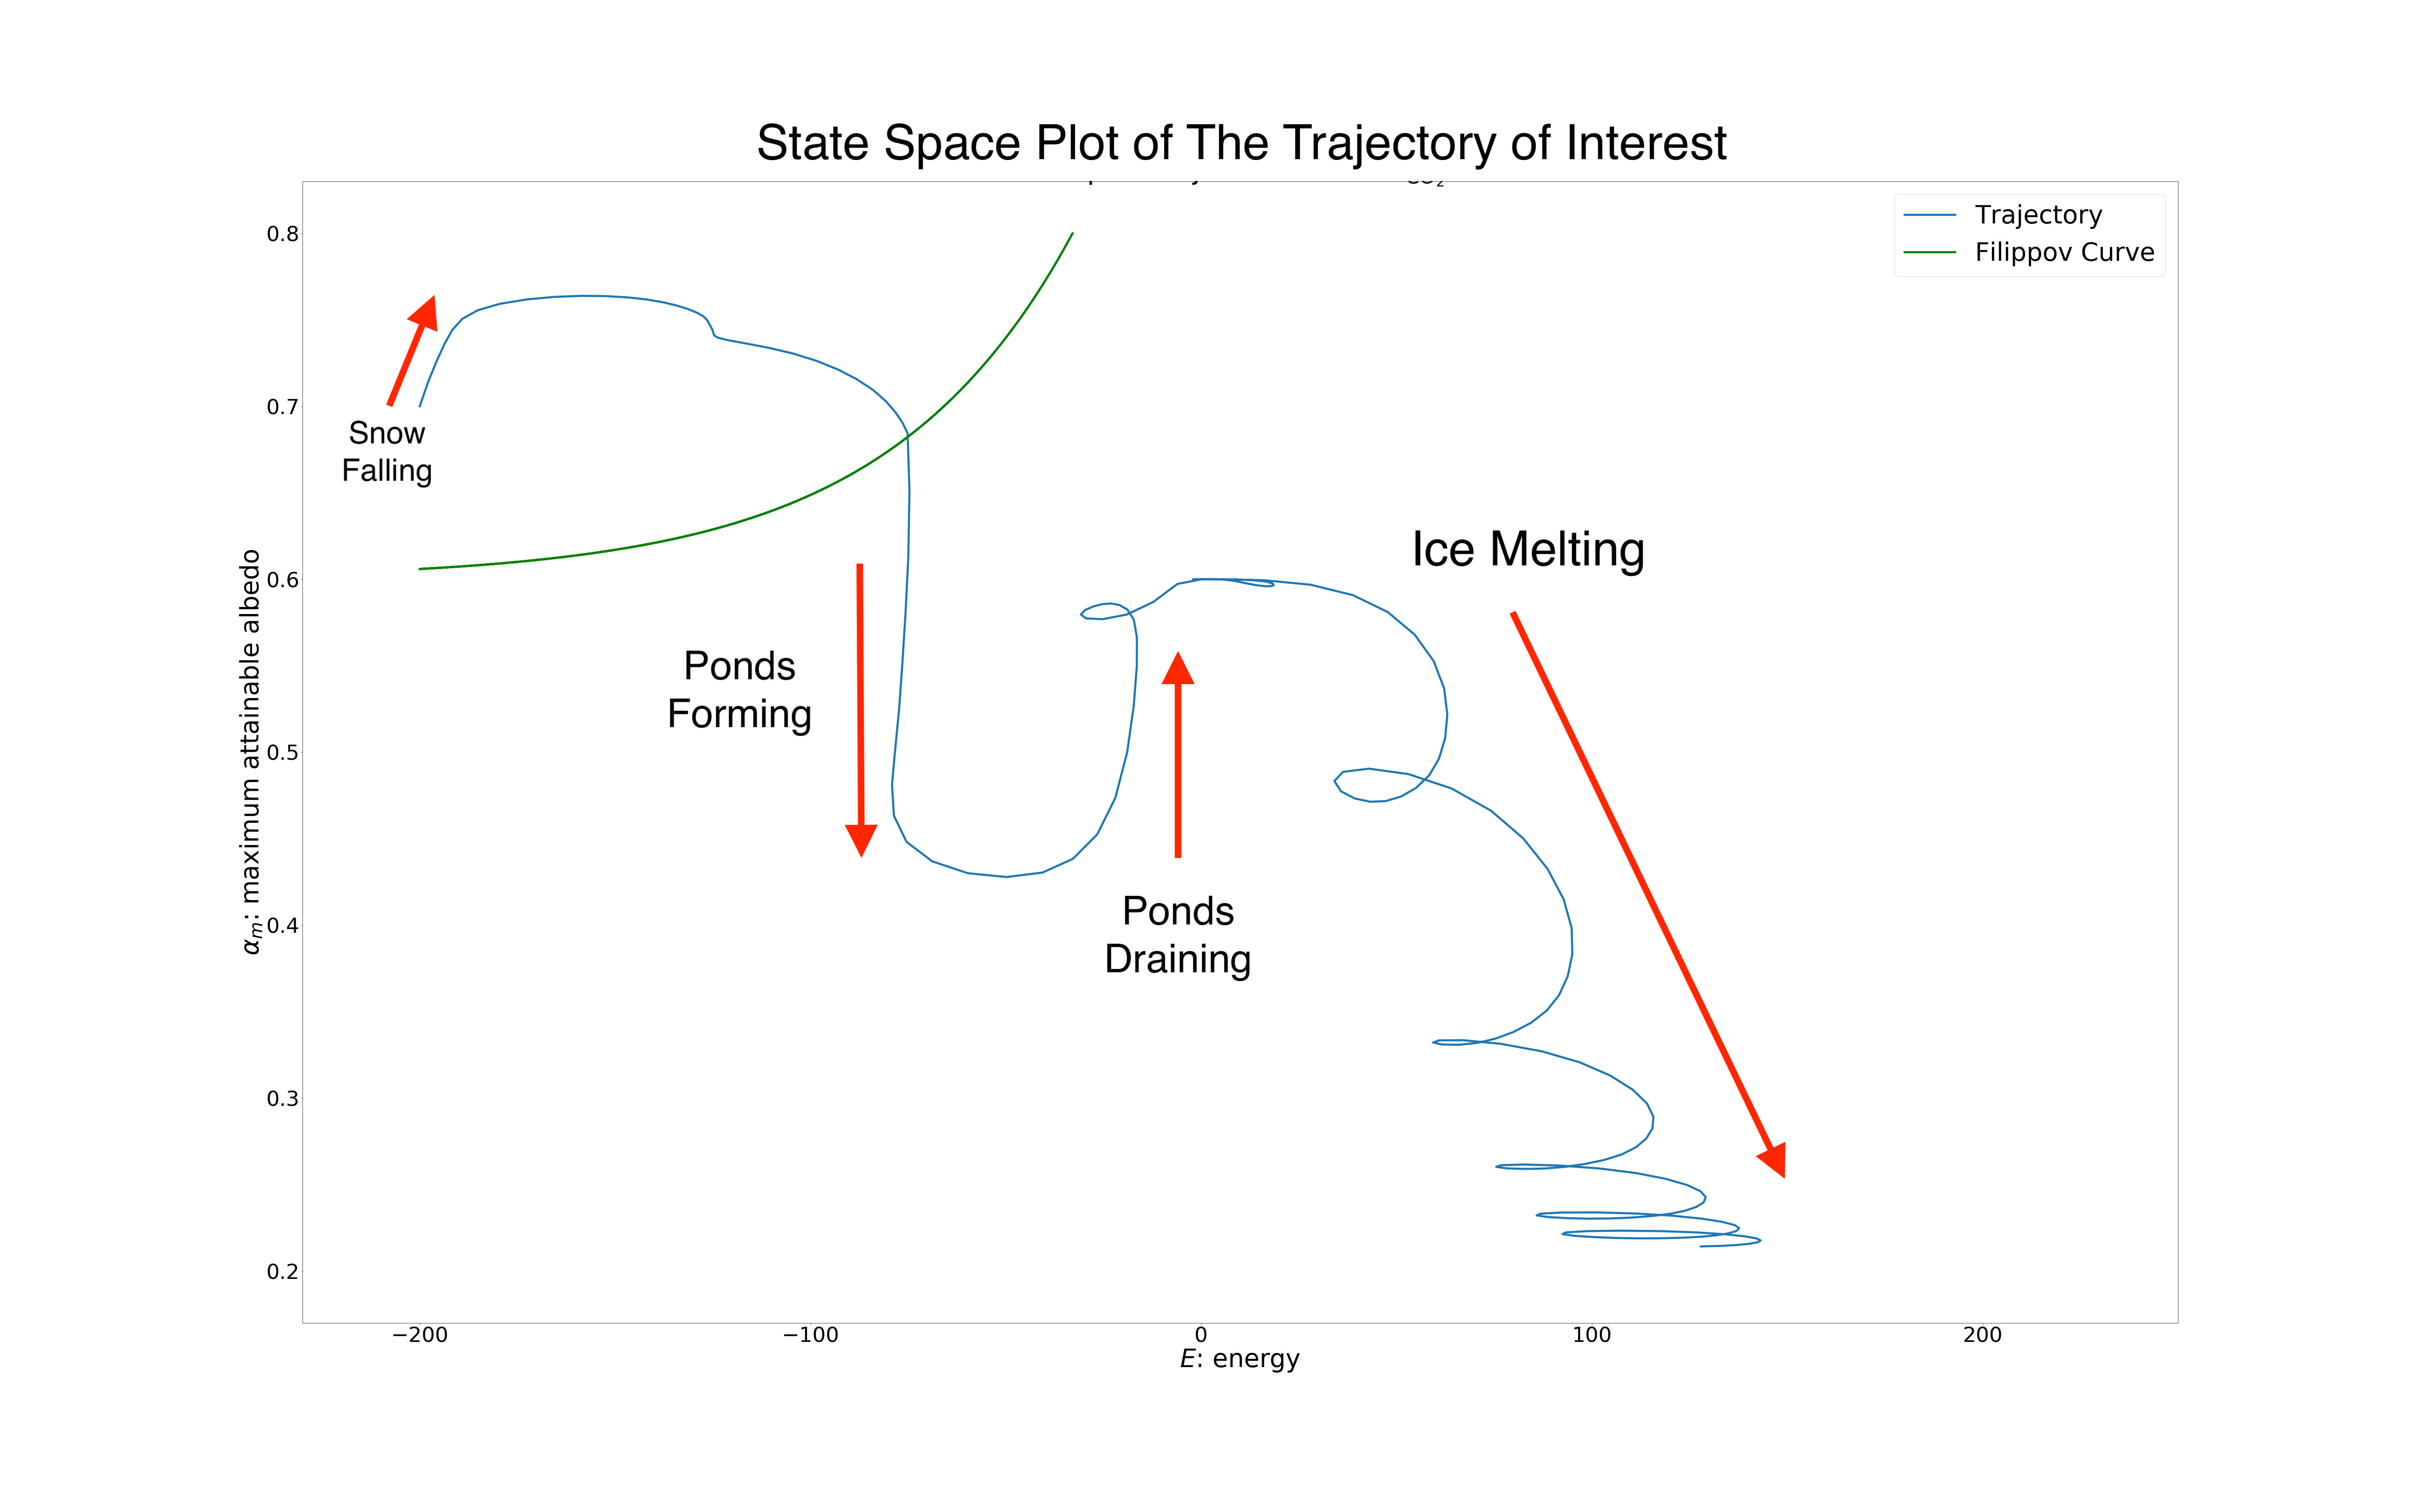
\includegraphics[width=\linewidth]{Figures/fc=60E=-200am=0_7.png} 
\end{center}
\caption{The state space trajectory that we use in data assimilation experiments.}
\end{figure}

\begin{itemize}
    \item In cold conditions, the system is at the left top part of the state space shown in \figref{onetrajectory}, where $\alpha(E,\alpha_m) > 0.6$. When the energy is largely negative, the logistic model term with the energy in the numerator dominates in \equref{coldalph}, and the maximum attainable albedo $\am$ rapidly approaches the carrying capacity of this term, $0.8$, representing the effect of snow falling. The initial rise from $0.7$ towards $0.8$ in \figref{onetrajectory} illustrates to this process. When the energy is close to zero, the term with the energy in the denominator (with the addition of 1 to avoid singularities at $E=0$) dominates, and $\am$ approaches $0.6$, which is not apparent from \figref{onetrajectory}. As the system's energy keeps increasing, it crosses the boundary between the two parts of dynamics.
    \item In warm conditions, the system is at the center part of the state space shown in \figref{onetrajectory}, where $\alpha(E,\alpha_m) < 0.6$. The rate that $\alpha_m$ approaches $0.2$ is faster when the energy is away from $0$ whereas the rate to approach $0.6$ is faster when the energy is near $0$. As a result, we take the energy to be in the denominator for the logistic model with a carrying capacity of $0.6$ and the energy in the numerator for the logistic model with a carrying capacity of $0.2$ \equref{warmalph}. In \figref{onetrajectory}, we can see that right after the system crosses the boundary, $\am$ is rapidly driven towards $0.2$, representing the process of ponding. When energy is higher, the ice becomes permeable, and melt pond drainage exposes the surface of the ice again, causing $\am$ to increase back to $0.6$ .
\end{itemize}

\par \figref{fczero} and \figref{fcsixty} plot the boundary curve and trajectories from various initial points in the state space with different values of $\fco$, respectively. When the value of $\fco$ is small, as in \figref{fczero} where $\fco=0$, the energy of the system stays negative, whereas when $\fco$ is sufficiently large, as in \figref{fcsixty} where $\fco=60$, the states that start with negative energy will cross zero and become positive. In our data assimilation experiments, we will focus on one particular trajectory of interest, the one with initial condition $E=-200$, $\am=0.7$ and parameter value $\fco=60$. The aforementioned \figref{onetrajectory} plots this trajectory along with the boundary curve separating the two parts of the dynamical system.

\begin{figure}\label{fig:fczero}
\begin{center}
\includegraphics[width=\linewidth]{Figures/fc=0_new.png} 
\end{center}
\caption{Trajectories with various initial points when $\fco=0$.}
\end{figure}

\begin{figure}\label{fig:fcsixty}
\begin{center}
\includegraphics[width=\linewidth]{Figures/fc=60_new.png} 
\end{center}
\caption{Trajectories with various initial points when $\fco=60$.}
\end{figure}

\par In terms of discrete time sequential data assimilation, the state variable is a two dimensional vector defined by
\begin{equation}\label{eq:xdef}
\mx = (E, \am )
\end{equation}
The model $\cM$ in \equref{DAmodel} is therefore defined by integrating the ODE \equref{coldalph} or \equref{warmalph} in time
\begin{equation}\label{eq:modeldef}
\cM(\mx_t,t) = \int_{t\Delta\tau}^{(t+1)\Delta\tau} \frac{d\mx}{dt} dt
\end{equation}
where $\frac{d\mx}{dt} = (\frac{dE}{dt},\frac{d\am}{dt})$, and $\Delta\tau$ is the time step in data assimilation. In our study, all the ODE's are numerically integrated using the Matlab program {\it disode45} \cite{disode45} with its default settings (the major algorithm parameters include absolute error tolerance $10^{-6}$ and relative error tolerance $10^{-4}$).

\section{Proxy for Ice and Pond Concentration and Satellite Radiances}\label{sec:radiancedef}

\par As mentioned in \secref{motivation}, for our particular problem, we need to define from our state variables $E$ and $\am$ proxies for other physical quantities of interest, including ice and pond concentration values, the satellite radiances, and satellite-retrieved ice concentration. In \equref{iceconcentration} We define the concentration of ice $C_i$ to be the one minus the percent difference between the physically highest attainable albedo of $0.8$ and the average of the maximum attainable albedo and the current albedo. The concentration here would approach 1 when the system is in a very cold state and the average is close to $0.8$.

\begin{equation}\label{eq:iceconcentration}
C_i(E,\am)=1-\left(\frac{0.8-\frac{1}{2}\left( \alpha_m+\alpha(E,\alpha_m)\right)}{0.6}\right)
\end{equation}

\par The pond concentration is defined as one minus the ratio of the current albedo to the maximum surface albedo. The idea here is that a low albedo at time $t$ compared to the maximum attainable albedo should mean the surface is covered in ponds. 

\begin{equation}\label{eq:pondconcentration}
C_p(E,\am)=(0.5\tanh(\frac{E+200}{10})+0.5)(1-\frac{0.2}{\alpha(E,\am)})^{1000}(1-\frac{\am}{0.8})
\end{equation}
%C_p(E,\am)=1-\frac{\alpha(E,\alpha_m)}{\alpha_m}

\par For the satellite retrieved concentration, to model the fact that the melt ponds obscure the microwave signature of the ice and thus melt ponds and open water are indistinguishable in terms of satellite radiances as mentioned in \secref{IntroRetrieval}, we take the maximum of zero and the difference between ice concentration and pond concentration.
\begin{equation}\label{eq:satelliteretrieval}
\csat(E,\am)=\max(0,C_i(E,\am)-C_p(E,\am))
\end{equation}

\figref{modelreview} plots the quantities of interest as they change with the state variables on the trajectory shown in \figref{onetrajectory} in the state space. \figref{modelreview2} gives plots of the time evolution of quantities of interest.

\begin{figure}\label{fig:modelreview}
\begin{center}
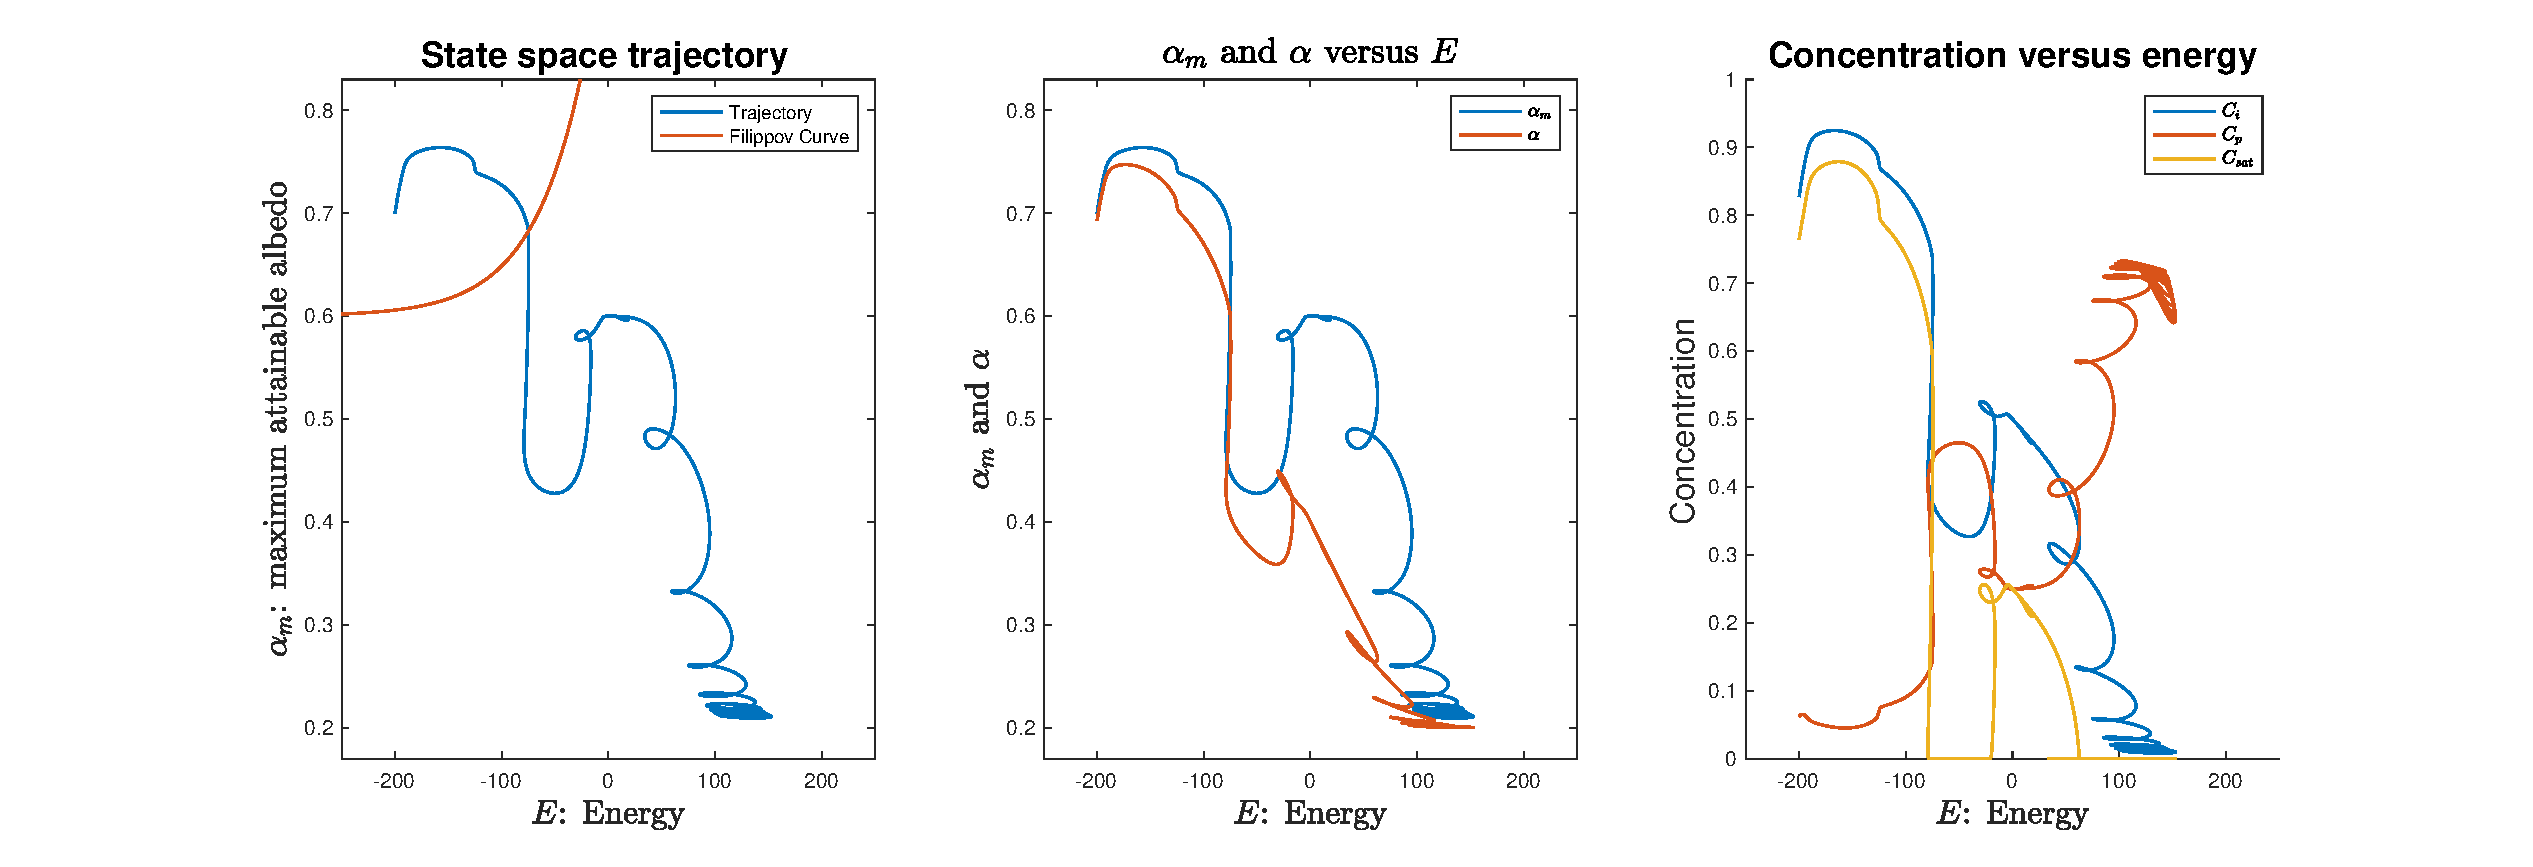
\includegraphics[width=\linewidth]{Figures/VersusEnergy.eps} 
\end{center}
\caption{Overview of the proposed proxy for the melt pond problem in sea ice concentration retrieval.}
\end{figure}

\begin{figure}\label{fig:modelreview2}
\begin{center}
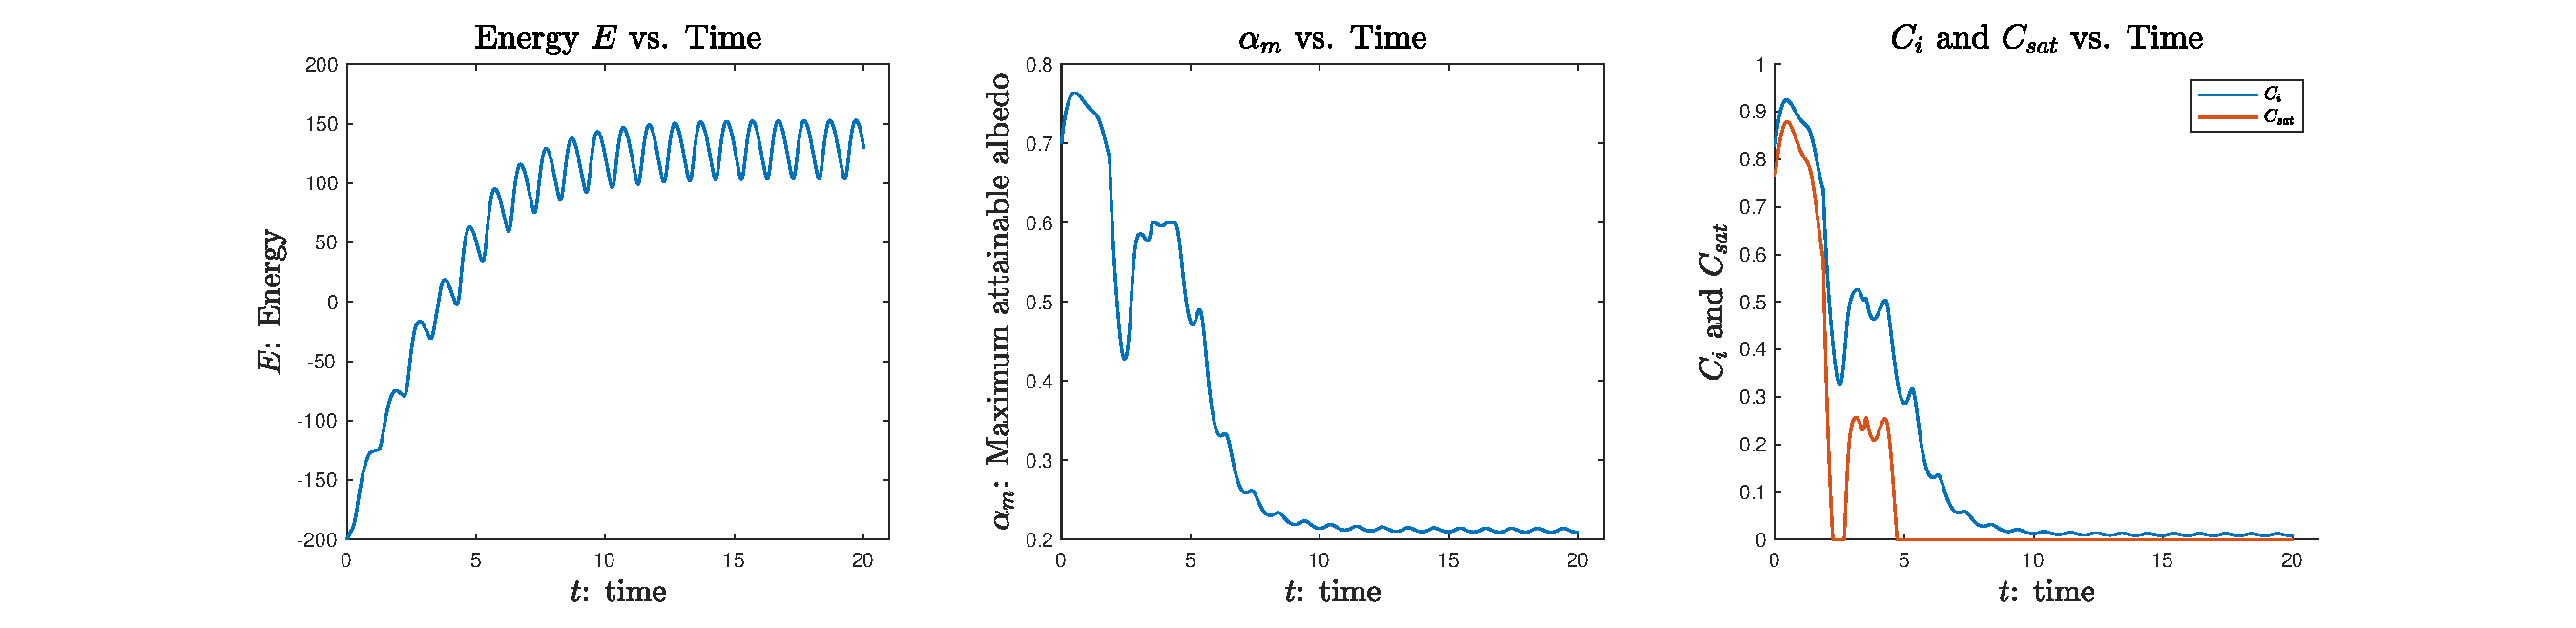
\includegraphics[width=\linewidth]{Figures/VersusTime.eps} 
\end{center}
\caption{Overview of the proposed proxy for the melt pond problem in sea ice concentration retrieval.}
\end{figure}

\par Finally, for the satellite radiances, we define functions of the state variables that give non-unique results around $E=0$, the energy where ponds form and drain. \figref{radversusenergy} plots the radiances as they change with the state variables on the trajectory shown in \figref{onetrajectory} in the state space. \figref{radversustime} gives plots of the time evolution of the five radiances.
\begin{equation}\label{eq:radiances}
\mO(E,\am) = 
\begin{bmatrix}
|E\alpha_m|\\ 
\alpha_m-\alpha(E,\alpha_m) \\
\alpha(E,\alpha_m)|E|\\
(0.5+0.4\tanh(\frac{50-E}{10}))(E+273.15)\\
C_i (1-\frac{\alpha(E,\alpha_m)}{\alpha_m})
\end{bmatrix}
\end{equation}

\begin{figure}\label{fig:radversusenergy}
\begin{center}
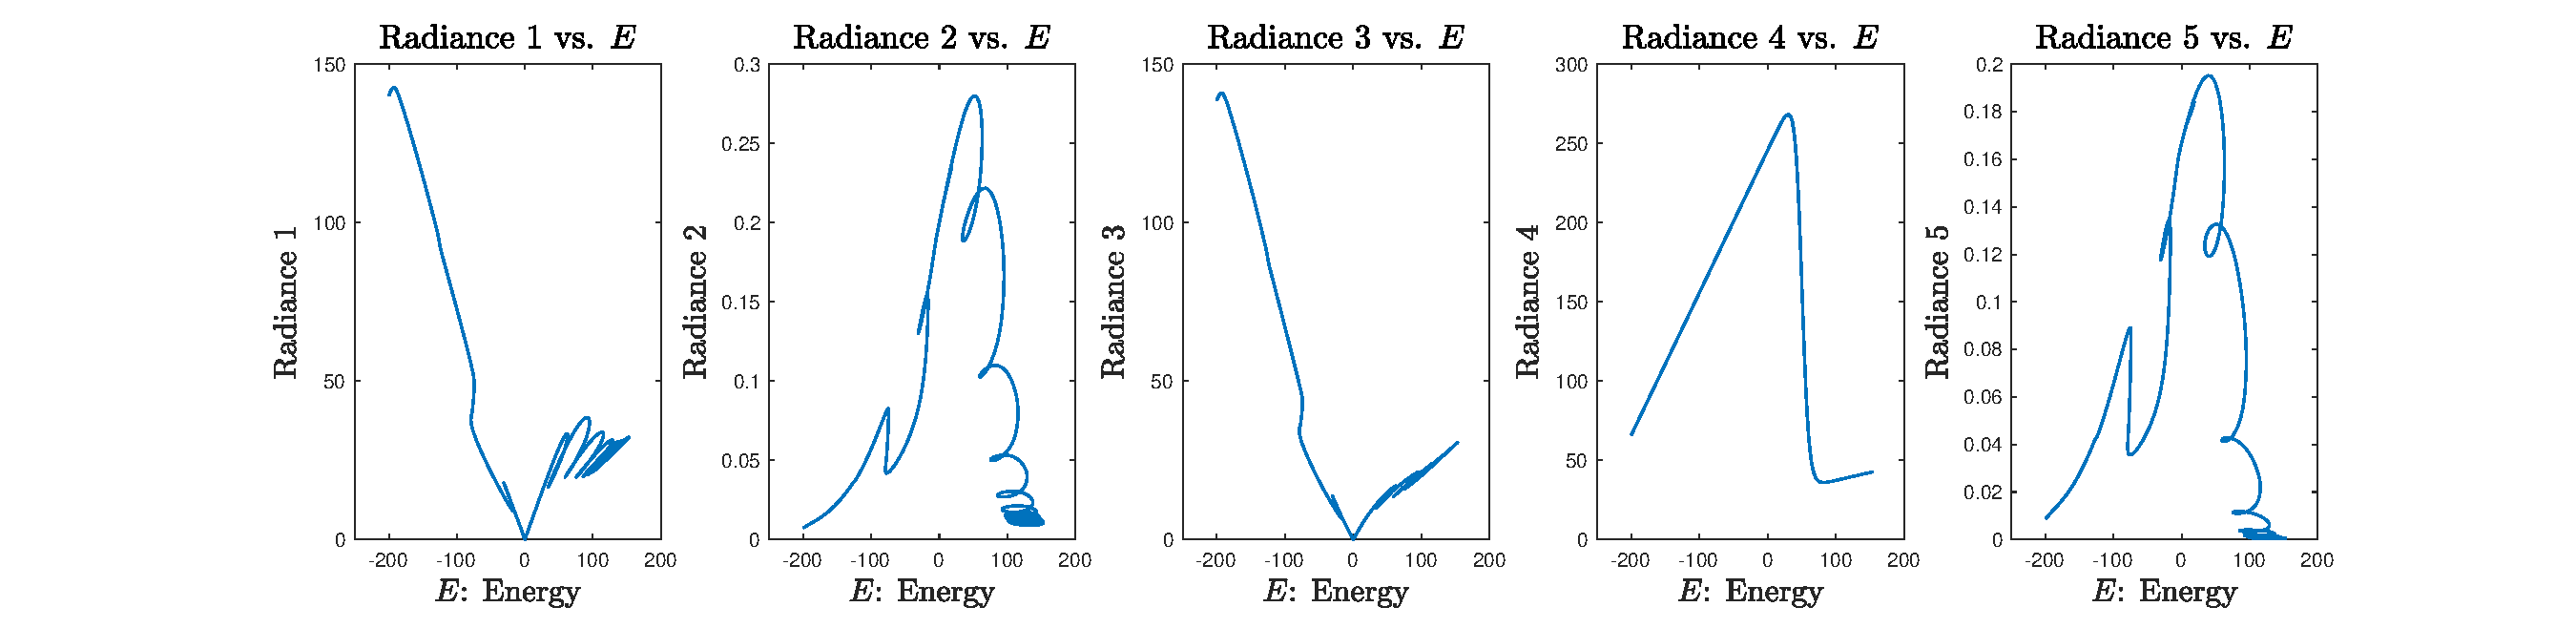
\includegraphics[width=\linewidth]{Figures/RadVersusEnergy.eps} 
\end{center}
\caption{The proxy for satellite radiances versus energy.}
\end{figure}

\begin{figure}\label{fig:radversustime}
\begin{center}
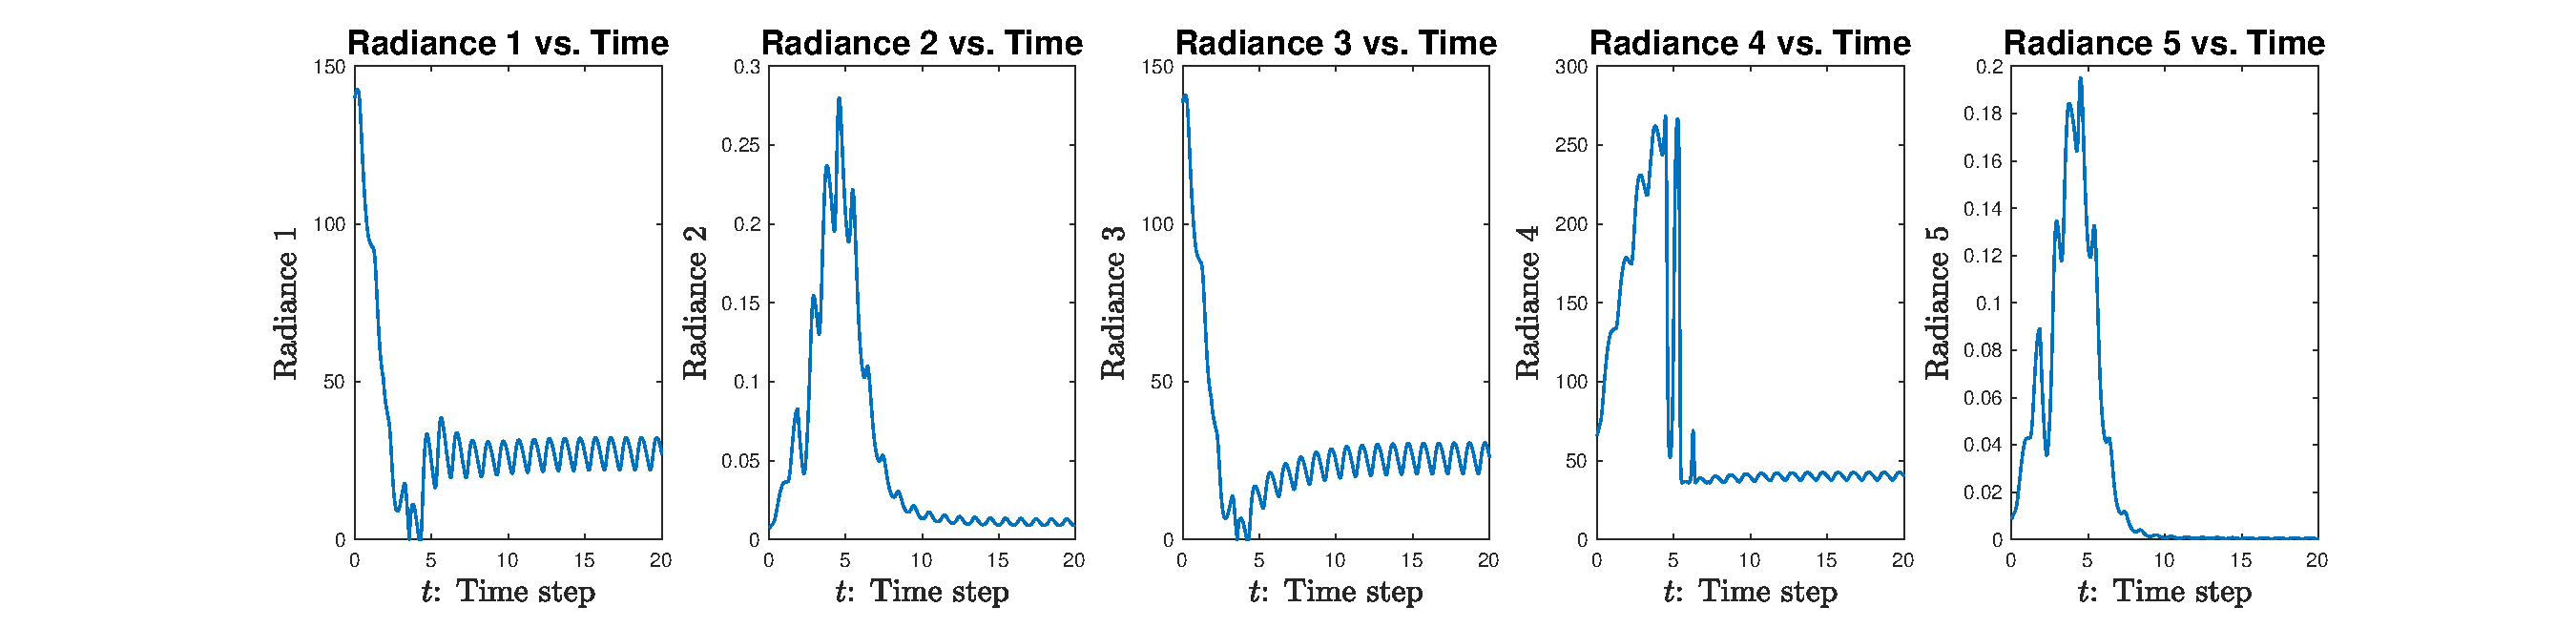
\includegraphics[width=\linewidth]{Figures/RadVersusTime.eps} 
\end{center}
\caption{The proxy for satellite radiances versus time.}
\end{figure}

\section{Problem of Using Satellite Retrived Concentration in DA}\label{sec:csatproblem}
\par In terms of data assimilation, if we assimilate with the satellite retrieved concentration, the real observation operator $\hsat$ generating the observations from state variables in \equref{DAobservation} would be the actual satellite retrieved ice concentration $\csat$ as a function of $E$ and $\am$ in \equref{satelliteretrieval}
\begin{equation}\label{eq:realcsat}
\hsat(\mx) = \hsat(E,\am) = \csat(E,\am) = \max(0,C_i(E,\am)-C_p(E,\am))
\end{equation}
However, since we think it is supposed to give the correct ice concentration, the observation operator $\hretrieval$ that is used to produce forecast output $\my_t^{f_i}$ in \equref{ensembleoutput} and \equref{ensembleupdate} would be the ice concentration $C_i(E,\am)$ as a function of $E$ and $\am$ in \equref{iceconcentration}
\begin{equation}\label{eq:supposedcsat}
\hretrieval(\mx) = C_i(E,\am) = 1-\left(\frac{0.8-\frac{1}{2}\left( \alpha_m+\alpha(E,\alpha_m)\right)}{0.6}\right)
\end{equation}
In this case, there is a systematic bias between $\hsat$ and $\hretrieval$. As discussed in \secref{IntroEnKF}, the apparent error in our knowledge about the observation operator $\cH$ could create severe problems in EnKF, and thus assimilate wrong information into our state estimate. Therefore, we propose to assimilate directly on satellite radiances with machine learned observation operator. In that case, our observation space is no longer the $1$-dimensional space of ice concentration, but the $5$-dimensional space of the satellite radiances. The real observation operator $\cH$ would be
\begin{equation}\label{eq:hreal}
\cH(\mx) = \cH(E,\am) = \mO(E,\am) = 
\begin{bmatrix}
|E\alpha_m|\\ 
\alpha_m-\alpha(E,\alpha_m) \\
\alpha(E,\alpha_m)|E|\\
(0.5+0.4\tanh(\frac{50-E}{10}))(E+273.15)\\
C_i (1-\frac{\alpha(E,\alpha_m)}{\alpha_m})
\end{bmatrix}
\end{equation}
While we do not have information of the specific form of the five functions in \equref{hreal} that make up $\cH$, we aim to find with machine learning a function $\hml\in C(\RR^2,\RR^5)$ that closely approximates $\cH$, that is
\begin{equation}\label{eq:hml}
\hml\approx\cH \quad \text{or} \quad \cH(\mx_t,t) - \hml(\mx_t,t) = \mxi_t
\end{equation}
where $\mxi_t$ is ideally an i.i.d sequence with $0$ mean and small variance. In this way, although there is still an error between $\hml$ and $\cH$, the systematic bias present in the case of $\hsat$ and $\hretrieval$ is gone. If $\mxi_t$ does behave like an i.i.d sequence with $0$ mean and small variance, we can incorporate this error as part of the uncertainty $\meps_t$ in the forecast model in \equref{DAmodel} or as part of the uncertainty $\meta_t$ in the observation in \equref{DAobservation}.
\begin{itemize}
    \item In \equref{ensembleoutput}, $\hml$ would be used to calculate $\{\my_t^{f_i}\}_{i=1}^{i=q}$, which are further used to estimate the Kalman gain. Without explicitly quantifying the error in the approximation of $\hml$ to $\cH$, we could think of this error as coming from the ensemble states $\{\mx_t^{f_i}\}_{i=1}^{i=q}$ instead of from $\hml$, since both uncertainty in $\{\mx_t^{f_i}\}_{i=1}^{i=q}$ and $\hml$ could could contribute to the uncertainty in $\{\my_t^{f_i}\}_{i=1}^{i=q}$. We will discuss this perspective in more details in \secref{inflation}.
    \item Furthermore, in \equref{ensembleupdate}, each ensemble member is updated with the Kalman gain and the difference between the observation and forecast output, where $\hml$ is used in place of $\cH$ in the equation. Here we could consider the uncertainty brought by $\hml$ as part of the uncertainty in the observations $\my_t$.
    \begin{equation}
    \my_t - \hml(\mx_t^{f_i}) = \my_t - \cH(\mx_t,t) + \mxi_t = \meta_t + \mxi_t
    \end{equation}
Originally, the observations are perturbed by $\cN(0,\mR_t)$ in \equref{perturbobservation} to account for uncertainty. Here we could account for this increased uncertainty from $\hml$ by first appropriately estimating $\mxi_t$ and further perturbing the observations accordingly. This is discussed in more details in \secref{inflation}.
\end{itemize} 

\chapter{Methods}
\section{Data Generation}\label{sec:datageneration}
\par To generate a data set for the training of machine learning observation operators, we first select points from the state space as \mX , calculate the corresponding radiances \mY, i.e. observations, and finally add error to the observations to get $\tilde{\mY}$. 

\paragraph{state space points} The first data set we generate is $\Dtraj$. To mimic the situation in the real world, we decide to use points on various trajectories in the phase space to form $\Xtraj$. From the model's formulation, the maximum attainable albedo $\am$ is only meaningful between $0.2$ and $0.8$, and the region of interest for $E$ is between $-200$ to $0$. Therefore, $20\times 30$ uniform grid data points from $S=[-200,0]\times[0.2,0.8]$ are chosen as initial conditions. \figref{fczero} and \figref{fcsixty} are in fact generated with such initial values with $\fco=0$ and $\fco=60$, respectively. Note that in our dynamical system \equref{coldalph} and \equref{warmalph}, the forcing parameter $\fco$ is also of interest. The real world analogy of $\fco$ would be the combined influence of total carbon dioxide emissions, different weather conditions, climate changes, and etc. Thus we should expect various values of $\fco$ in the data set. To capture this effect, we generate trajectories with $12$ values of $\fco$ ranging from $-10$ to $100$. The model is run for $200$ time steps with a step length of $0.05$ for each initial condition and each value of $\fco$, resulting in $2400$ trajectories and $1440000$ data points. From the data points, $\Ytraj=\cH(\Xtraj)$ are calculated and noises are added to give $\Ytrajtil$. $\Xtraj$ and $\Ytrajtil$ form the data set $\Dtraj=(\Xtraj,\Ytrajtil)$.

\paragraph{grid data points} From \figref{fczero} and \figref{fcsixty}, we can see that in places where the limit cycles exist, the trajectories are clustered and the data is dense in that region, whereas in places where the trajectories go through transient states, the data is sparse. As we will later demonstrate in \secref{DataDensity}, such imbalance creates a problem for the machine learning algorithm. To fully exploit the potential of the machine learning algorithm to fit the satellite radiances, we also generate a data set with the unrealistically large amount of data filling up the whole state space. $2000\times 3000$ uniform grid data points from $S=[-200,0]\times[0.2,0.8]$ are chosen to form $\Xgrid$. From the data points, $\Ygrid=\cH(\Xgrid)$ are calculated and noises are added to give $\Ygridtil$. $\Xgrid$ and $\Ygridtil$ form the data set $\Dgrid=(\Xgrid,\Ygridtil)$.. We expect that with sufficient data, the machine learning algorithm should perform well everywhere in the state space.

\paragraph{observations and error} The observations are calculated for each of the generated data points with \equref{radiances}. In the real world, the data is never perfectly clean, so it is important to add error in the observations. Moreover, the machine learning algorithms are expected to average out the white noise error and learn the true pattern behind the noises. Note that the five radiances have different magnitude scales, radiance 1,3,4 are of $\sim 10^1$ while radiance 2,5 are of $\sim 10^{-2}$. We initially did not take such effect into account and add the same error $\cN(0,1)$ to all five radiances. Experiments showed that machine learning algorithms were not able to learn anything about radiance 2,5. We also tried to add error proportional to the value of each radiance at each point. However, this approach created a problem for values near $0$, in which case essentially no error is present. Our final approach is adding error proportional to the mean absolute value of each radiance.
\begin{align}
\bar{y}_j & = \sum_{i=1}^n | y_{ij} | \label{def:ybar}\\
\tilde{y}_{ij} &= y_{ij} + \eta_{ij} \label{def:ytilde}\\
\eta_{ij} &\sim \cN(0,\lambda \bar{y}_j) \label{def:eta}
\end{align}
where $\lambda$ is a control parameter for the magnitude of the error. We generate 7 datasets with $\lambda \in \{ 0,0.1,0.2,0.3,0.4,0.5,0.6\}$ to investigate how error affects machine learning algorithms. In data assimilation, we also use the same approach to add error to observations.

\section{Model Training and Selection}
\par Since we construct the function for satellite radiances $\cH$ in a highly nonlinear manner, we decide to use the artificial neural network (ANN) as the machine learning algorithm. Other algorithms such as XGBoost and Random Forest are also worth experimenting in the future. We split the data set randomly into $90\%$ for training and validation, and $10\%$ for evaluation. We also exclude from the training set the points on the trajectory that we will use in the DA experiment to avoid overfitting. The training-validation set is further split into the training set and validation set. We choose hyperbolic tangent $\tanh$ as the activation function in hidden layers. We add batch normalization \cite{BatchNorm} before each hidden layer and dropout \cite{Dropout} after each hidden layer to regularize the network and prevent it from overfitting. All parameters are initialized using Xavier initialization \cite{Xavier}. The network is trained with Adam optimizer \cite{Adam}. Hyperparameters are chosen based on 9-fold cross-validation. The network is implemented in Python with Keras framework using Tensorflow as backend. After experiments, we choose four layers to get our architecture shown in \figref{FNN}. The machine learning model can be written as a composed function in \equref{ourml}

\begin{equation}\label{eq:ourml}
\vy = \vx_{\text{out}} = \vW_4(\tanh(\vW_3(\tanh(\vW_2(\tanh(\vW_1 \vx_{\text{in}} + \vb_1))+\vb_2))+\vb_3))+\vb_4
\end{equation}
where $\tanh$ is the element-wise hyperbolic tangent function, $\vW_2,\vW_3,\vW_4$ are $5\times 5$ matrices, $\vW_1$ is a $5\times 2$ matrix and $\vb_1,\vb_2,\vb_3,\vb_4$ are $5$-dimensional vectors. The total number of parameters is $105$. The parameters are determined by the optimization algorithm.

\begin{figure}\label{fig:FNN}
\begin{center}
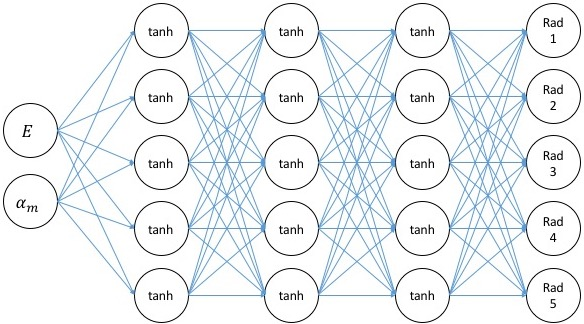
\includegraphics[width=0.85\linewidth]{Figures/FNN.jpeg} 
\end{center}
\caption{Graphical representation of the proposed machine learning model.}
\end{figure}

\section{Evaluation}\label{sec:MLeval}
\par To examine the accuracy of the prediction model, two evaluation measures are used in this study: Root Mean Square Error (RMSE) and Mean Absolute Percentage Error (MAPE). They are defined as:
\begin{align}
\text{RMSE} & = \sqrt{\frac{1}{nm}\sum_{i=1}^n\sum_{j=1}^m(y'_{ij}-y_{ij})^2} \\
\text{MAPE} & = \frac{1}{nm}\sum_{i=1}^n\sum_{j=1}^m\bigg|\frac{y'_{ij}-y_{ij}}{y_{ij}}\bigg|
\end{align}
where $y_{ij}$ is the $j$th feature of the $i$th sample, $y'_{ij}$ is the predicted value of the corresponding $y_{ij}$.

\par \figref{MLevaluation} plots the points on the trajectory that we will use in the DA experiment and the corresponding values of radiance 1,2,4 on those points. \figref{MLrad1} is a larger illustration of the lower left plot of \figref{MLevaluation}. The figures compare the values given by machine learning algorithm $\hml(\mX)$ with the truth $\mY$ and the noisy training data $\tilde{\mY}$ with $\lambda=0.4$. In most places, the machine learning values overlap with the truth and give reasonable values in general. Particularly, it seems that machine learning is able to average out the noise and discover the real pattern in the data. In the lower middle plot of the 4th radiance value, even though the noise in the training data is disproportionately large, our machine learning model is still able to recover the true values behind the noise. In fact, through experiment, we found out that, with appropriate techniques and sufficient data, machine learning is not severely affected by the amount of noise in the training data. The model trained with $\lambda=60\%$ is only slightly worse than the model trained with $\lambda=0\%$. Besides, the performance of the benchmark machine learning model $\hmlhat$ trained with a large amount of data is almost perfect, as we expected. The plot is not shown since the machine learning values virtually overlap with the truth everywhere. In some sense, we can safely say that the machine learning algorithm fit the function perfectly and should be identical as and indistinguishable from the true function $\cH$. The accuracy of $\hml$ and $\hmlhat$ satisfies our assumption in \equref{hml} that the error in the machine learned observation operator should be white noise with zero mean and small variance.

\begin{figure}\label{fig:MLevaluation}
\begin{center}
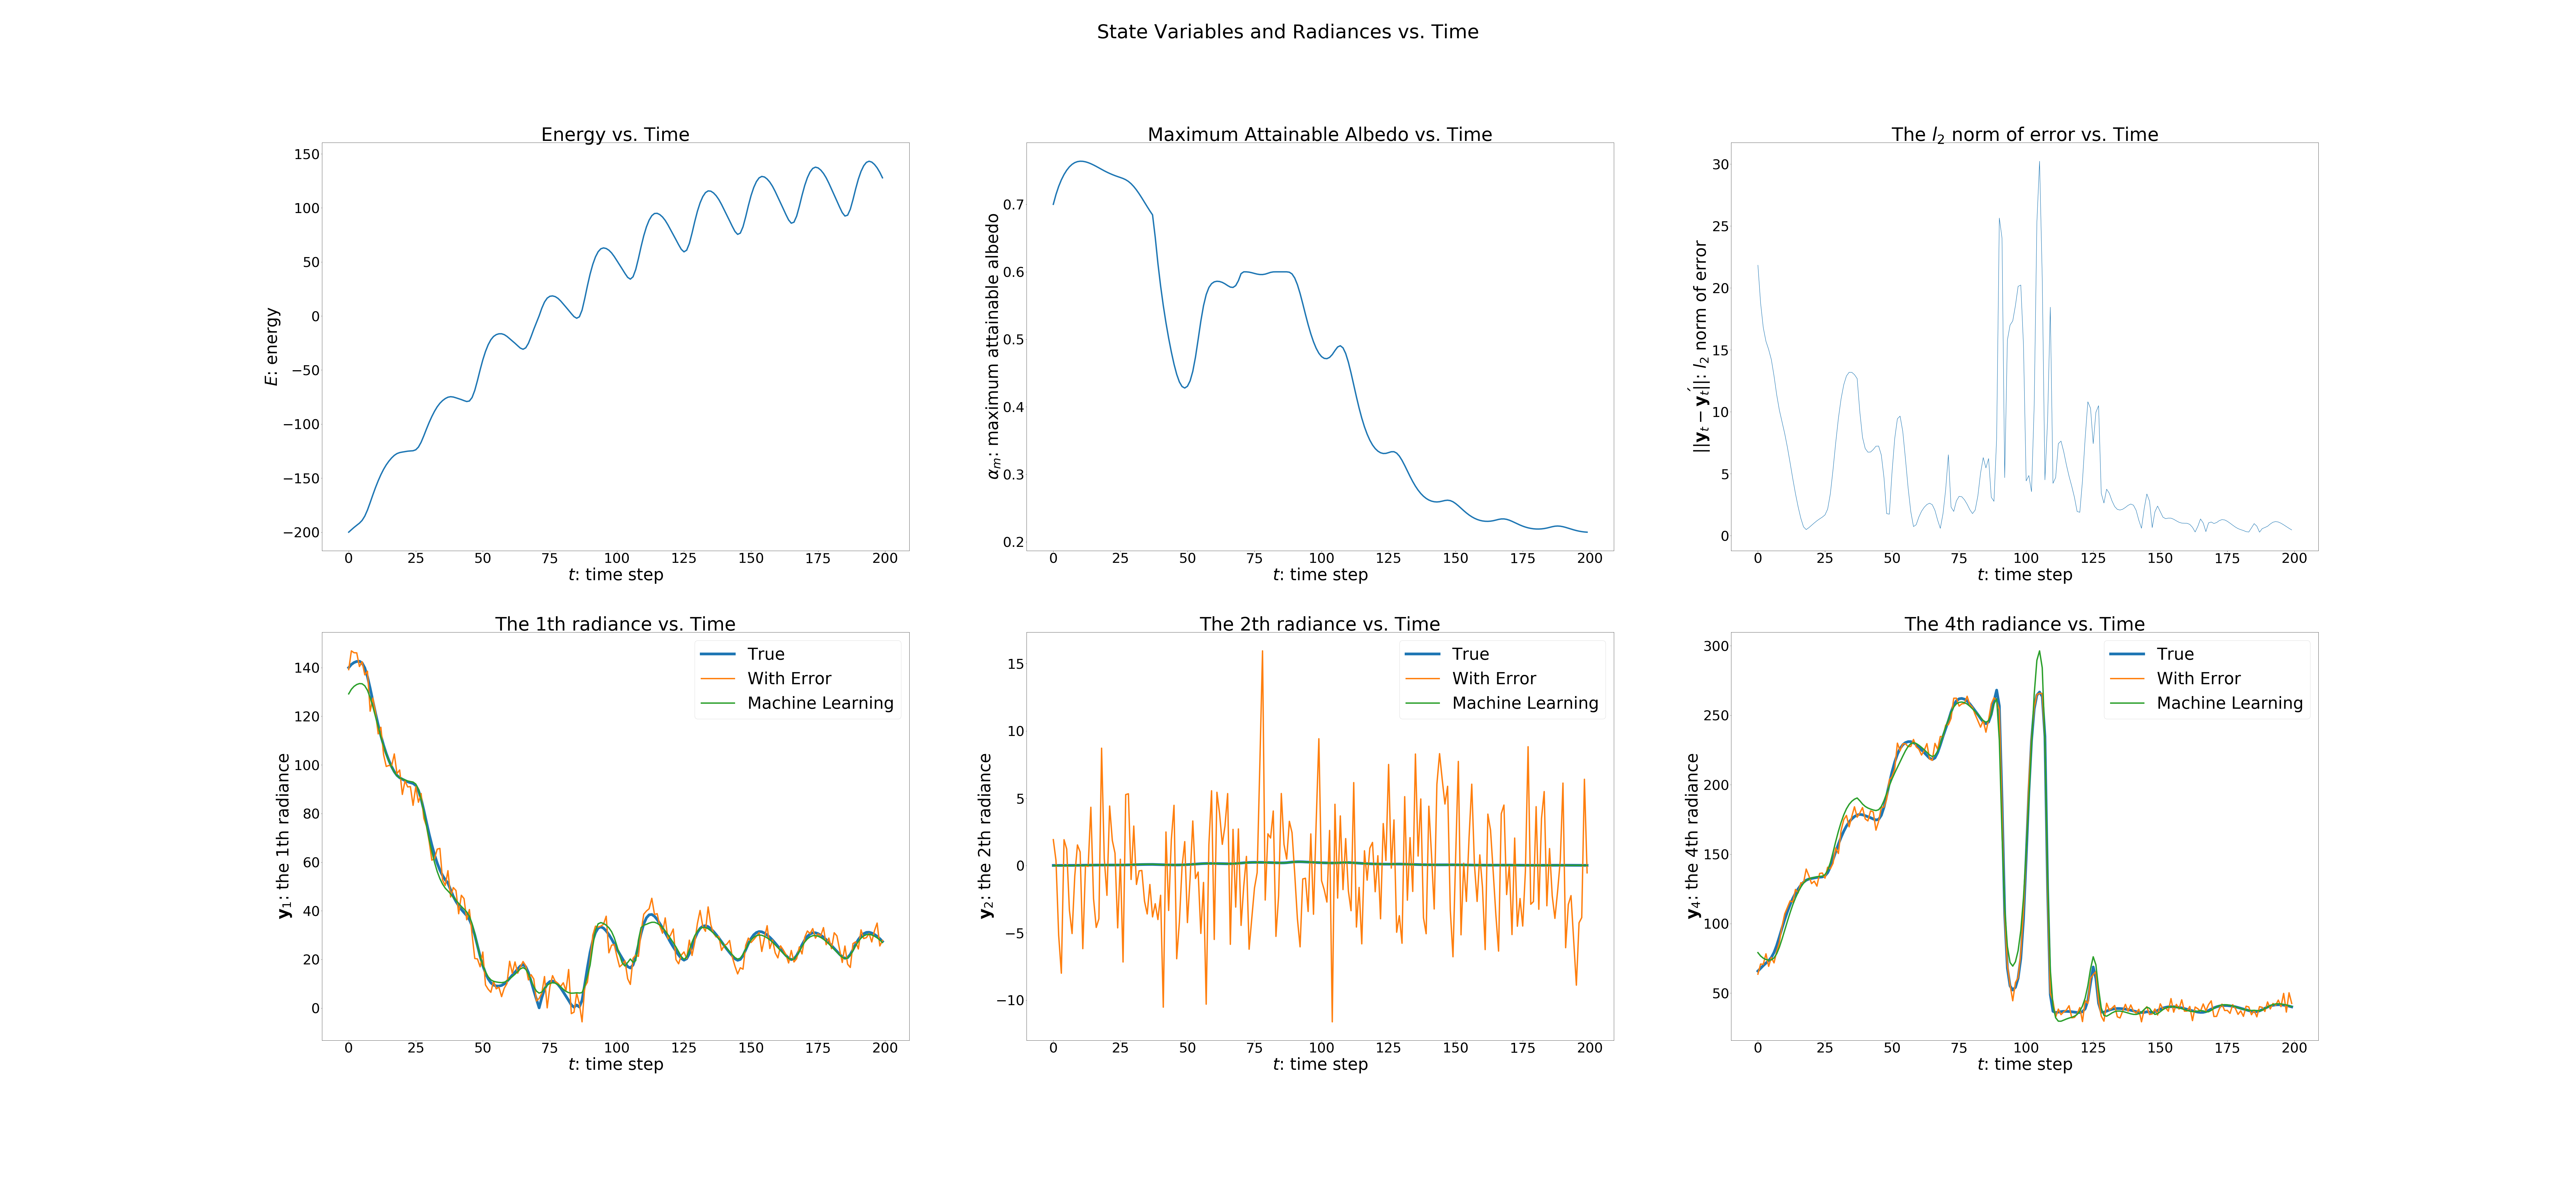
\includegraphics[width=\linewidth]{Figures/StateAndRadiances_2.png} 
\end{center}
\caption{The performance of machine learning observation operator evaluated on one trajectory.}
\end{figure}

\begin{figure}\label{fig:MLrad1}
\begin{center}
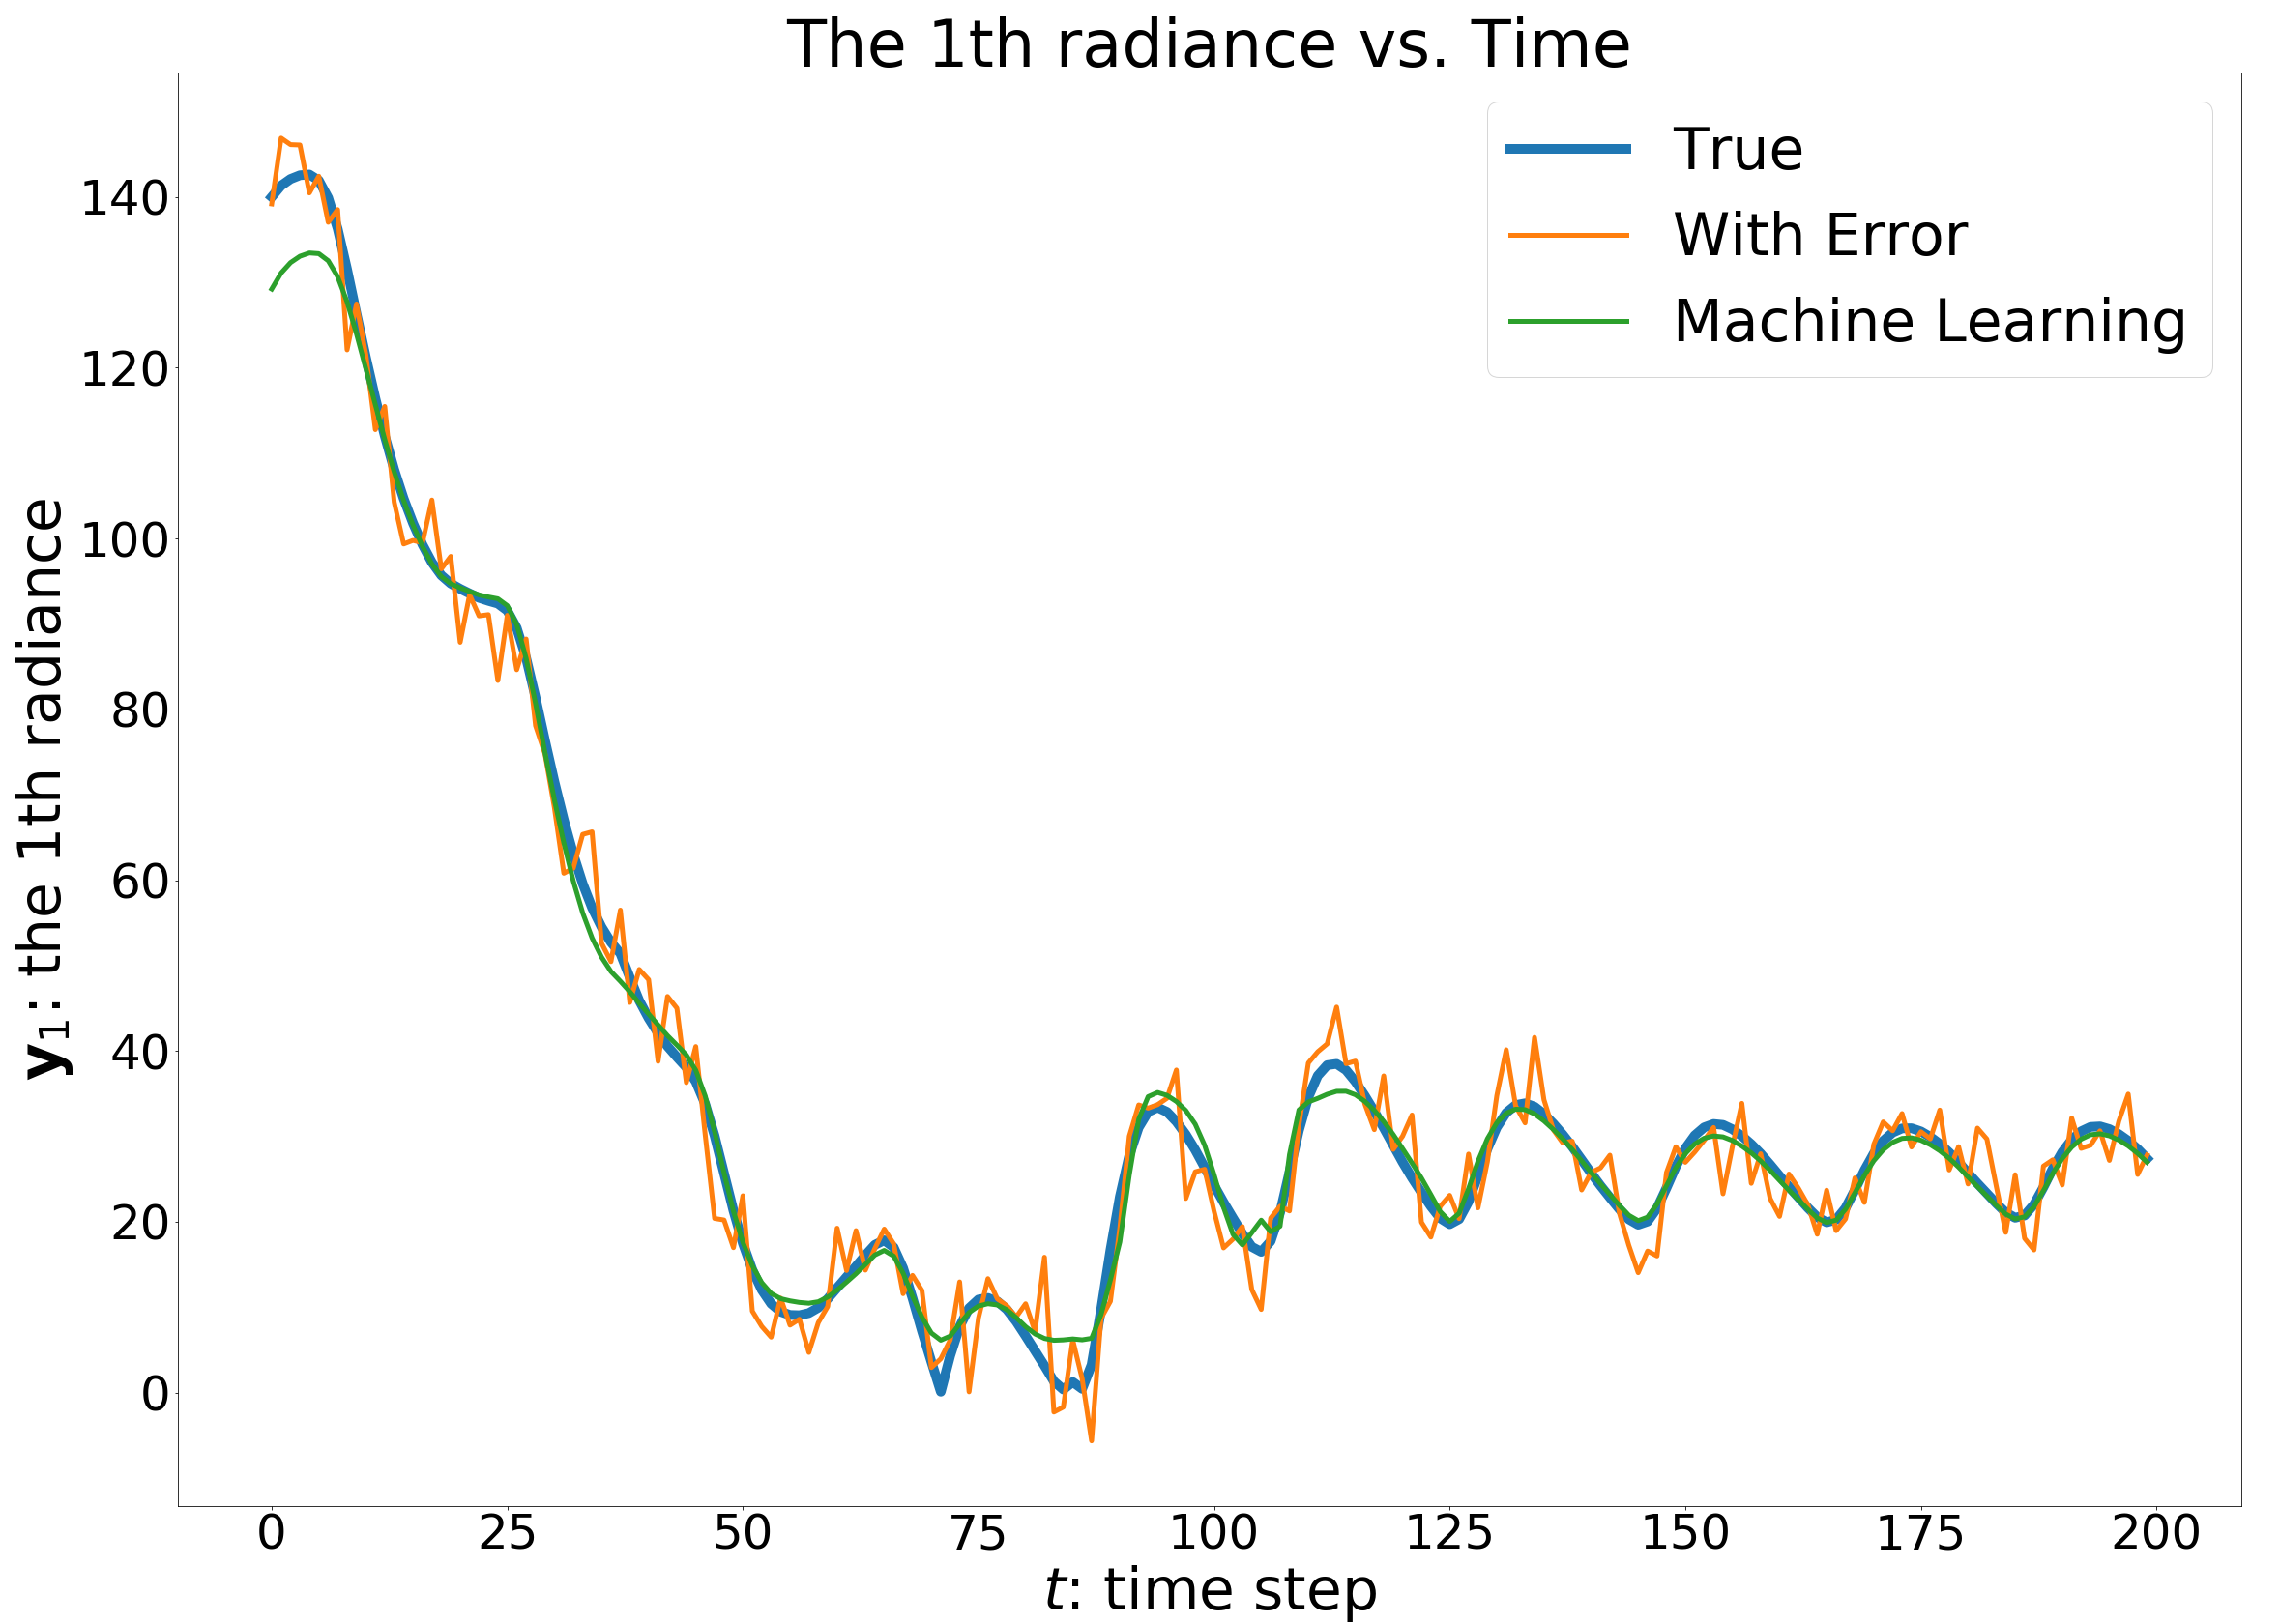
\includegraphics[width=0.85\linewidth]{Figures/StateAndRadiance1.png} 
\end{center}
\caption{Time evaluation of the 1st radiance, true value, noisy value and ML fitted value.}
\end{figure}

\subsection{Data Density}\label{sec:DataDensity}
\par Although in general machine learning achieves a high level of accuracy, $\hml$ displays different levels of error in different parts in the state space. It is well known that the amount of available training data is a significant factor in determining the performance of machine learning algorithms. In our study, since we generate data with trajectories for $\hml$, the data points are not uniformly distributed spatially. In regions where the system achieves equilibrium states and where limit cycles exist, the data points are clustered together and we therefore have a large amount of data to train the machine learning algorithm. In regions where the system goes through transient states, the data points are sparse and we have a limited amount of data to train the machine learning algorithm. The experiments show correlation between the accuracy and the amount of available training data, or data density, in different regions in the state space. To demonstrate this correlation and to quantify the expected error in different regions, we divide the state space into $45\times 30$ uniform grids, with each grid square representing $10$ units in energy $E$ and $0.02$ unit in maximum attainable albedo $\am$. In each grid square, we sum up the number of data points in the training data (and then take logarithm) to represent the data density in this square region. We take the averaged RMSE of all the values in the grid square to serve as the expected error estimation in that region. \figref{densitymatrix} is a heat map plot of the density in the grid regions, where the color bar represents the logarithm of the number of available data points in each grid. \figref{errormatrix} is a heat map plot of the expected error in the grid regions, where the color bar represents the averaged RMSE.

\begin{figure}\label{fig:densitymatrix}
\begin{center}
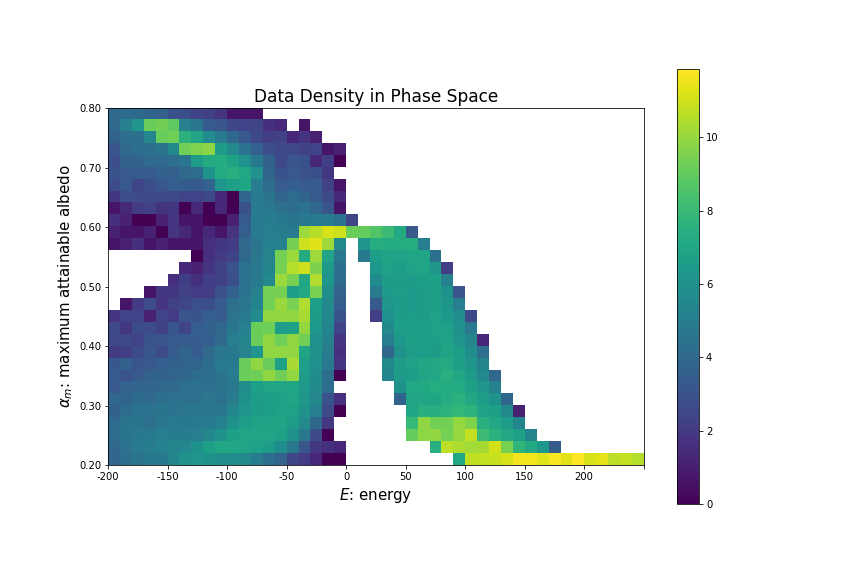
\includegraphics[width=\linewidth]{Figures/DensityMatrix.png} 
\end{center}
\caption{Density of available training data for machine learning in the state space.}
\end{figure}

\begin{figure}\label{fig:errormatrix}
\begin{center}
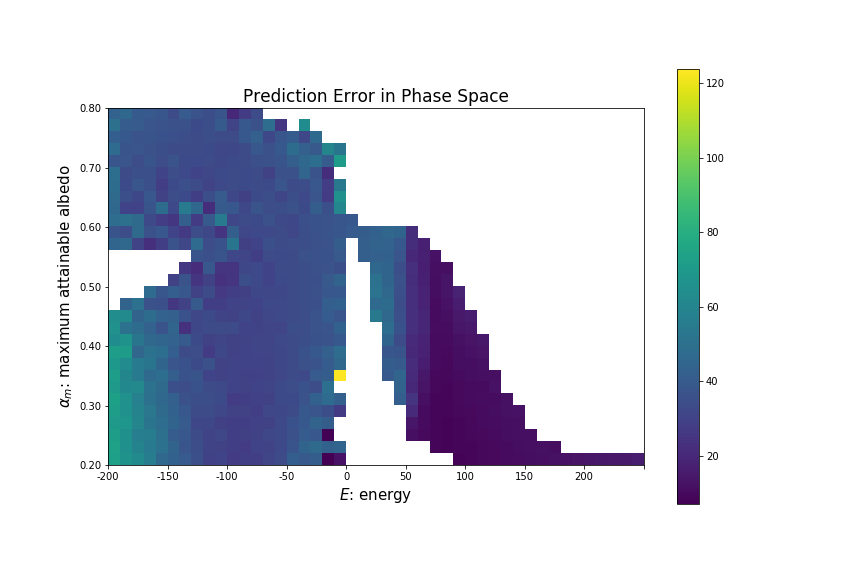
\includegraphics[width=\linewidth]{Figures/ErrorMatrix.png} 
\end{center}
\caption{Error of machine learning algorithm in state space.}
\end{figure}

\par From the plots, we can see the correlation between data density and error. The darker blue colors in \figref{densitymatrix} roughly correspond to the lighter green-yellow colors in \figref{errormatrix}. In particular, for the equilibrium states, where sufficient training data exists, our model tends to perform quite well, whereas for the transient state, where training data is extremely sparse, the values given by machine learning does not make much sense. As previously described in \secref{csatproblem} and \equref{hml}, we expect the difference between $\hml$ and $\cH$ to be an i.i.d. sequence with 0 mean and small variance. However, as the state variables evolve in the state space, the error $\mxi$ also varies. To address this issue in data assimilation, we consider $\mxi$ as a function of the state variables $E$ and $\am$, and estimate $\mxi(E,\am)$ with the averaged RMSE error and data density in the corresponding grid square. Then we apply appropriate covariance estimation and inflation. The details are discussed later in \secref{inflation}.

\subsection{Training with Sparse Data}\label{sec:sparsedata}
\par As discussed above, data density plays a significant role in determining the accuracy of the machine learning algorithm in different regions in the state space. In the real world, different regions of the state space represent different physical configurations of the system. It is completely possible that the current states of the system are rarely seen in the past and thus the machine learning algorithm does not have sufficient historic data to learn the behavior of observation operator in such situation. To further investigate the influence of sparse training data in the region of interest, we generate another two data sets, where we have limited training data in a certain region, and train another two machine learning observation operator with these data sets respectively. We are most interested in the region $S=\{(E,\am):E\in[-50,50]\}$, shown in \figref{sparsephase} as the shaded region, where the energy crosses zero and the interesting dynamics corresponding to pond forming and draining happens. From the data set $\Dtraj$, we randomly drop $95\%$ ($70\%$, respectively) of the data from $\Xtraj$ in the region $S$ and the corresponding observations from $\Ytrajtil$ to significantly decrease the amount of available training data in that region. The resulting data sets are $\Dsparser=(\Xsparser,\Ysparsertil)$ (and $\Dsparse=(\Xsparse,\Ysparsetil)$, respectively).

\begin{figure}\label{fig:sparsephase}
\begin{center}
\includegraphics[width=\linewidth]{Figures/sparse.png} 
\end{center}
\caption{Drop out data in the shaded region of interest.}
\end{figure}

\par After training our neural network with $\Dsparser$ and $\Dsparse$, we get two machine learning observation operators $\hsparser$ and $\hsparse$. They are again evaluated and analyzed with the same methods described in \secref{MLeval}. \figref{sparsedensitycomparison} compares the original data density of $\Dtraj$ and the data density of $\Dsparser$ after dropping $95\%$ data in $E\in[-50,50]$. \figref{sparseerrorcomparison} compares the accuracy of $\hml$ and $\hsparser$. There is a clear boundary in both figures - inside the region $S$ where data is dropped, data is apparently sparser and the error is significantly larger than outside the region. We can clearly see that with only $5\%$ of the data, our neural network starts to make mistakes.

\begin{figure}\label{fig:sparsedensitycomparison}
\begin{center}
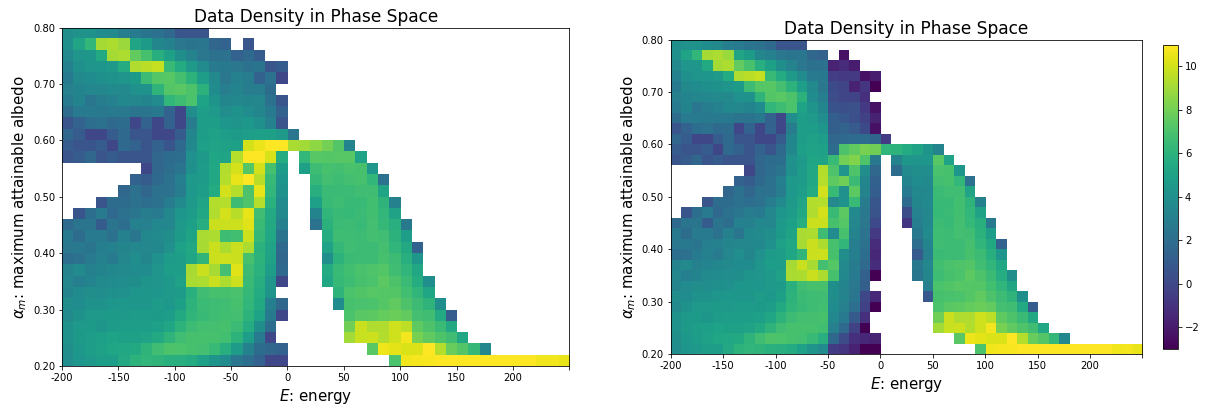
\includegraphics[width=\linewidth]{Figures/DensityMatrix_sparse_comparison.png} 
\end{center}
\caption{Comparison between the original data density (left) and the data density after dropping $95\%$ data in $E\in[-50,50]$.}
\end{figure}

\begin{figure}\label{fig:sparseerrorcomparison}
\begin{center}
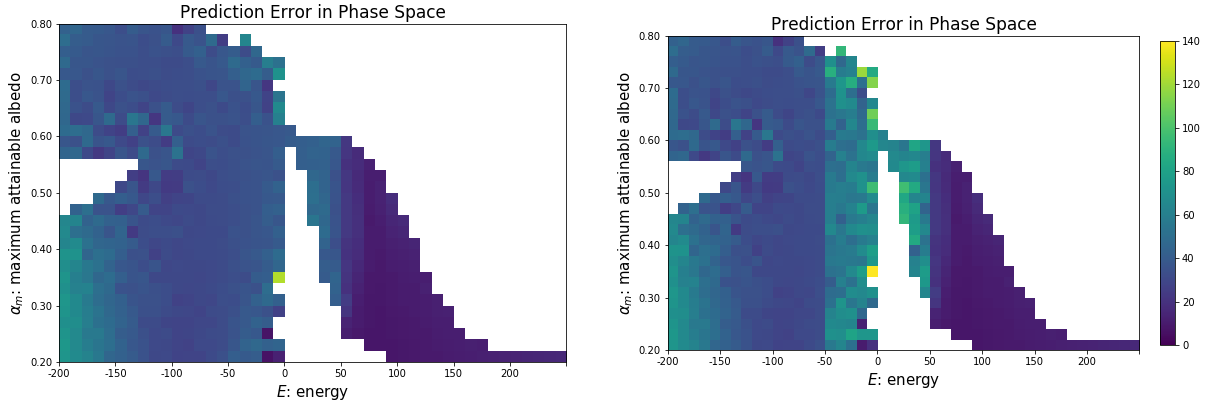
\includegraphics[width=\linewidth]{Figures/ErrorMatrix_sparse_comparison.png} 
\end{center}
\caption{Comparison between the error of machine learning algorithm with all data (left) and with $5\%$ data in $E\in[-50,50]$.}
\end{figure}

\chapter{Experiments}\label{ch:experiments}

\section{Setup}\label{sec:expsetup}
\par In this chapter, we test our machine learning observation operator in the data assimilation scheme. The state variable in the experiment is $\mx=[E,\am]$. The model that evolves the states in time $\cM$ is defined by \equref{coldalph} and \equref{warmalph}. To focus on the observation operator, we adopt the perfect model assumption in our experiment, i.e. assume we know the true model and exclude any model error from our experiment. Therefore the forecast model dynamics is the same as the true dynamics. The time step is set as $0.05$, which roughly corresponds to 18 days in the physical sense, allowing us to see the seasonal effects brought by the seasonally varying terms in the model $F_T(t)$, $F_0(t)$, and $F_s(t)$. The experiment lasts for $200$ steps, i.e. $10$ years, after which no further interesting behaviors can be observed from the experiments. The true observations are generated by \equref{radiances} in most experiments and by \equref{satelliteretrieval} in the experiment with $\hretrieval$. We assume that the observations are available at every time $t$. We also add noise to the true observations the same way we add error to the training data in \equref{yf}, \defref{ytilde}, and \defref{eta}, with $\lambda=20\%$. Data assimilations are done at every integration time $t_n$. The analysis error is defined as the $l_2$ norm of the difference between the true value and the analysis.
\par The true initial condition is $\mx_0=[0.7,-200]$, i.e. $E_0=-200$ and $\alpha_{m_0}=0.7$, with $\fco=60$, from which \figref{onetrajectory} is generated. The initial ensemble mean is a perturbed value from the true initial condition:
\[\bar{\mx}^f_0 = \mx_0+\cN(0,\begin{bmatrix}
    0.12 & 0 \\
    0 & 40
    \end{bmatrix})
\]
The initial spread is defined as 
\[\mP^f_0 = \begin{bmatrix}
    0.12 & 0 \\
    0 & 40
    \end{bmatrix}
\]
The size of the ensemble is taken as 100. Through experiments, we found that a larger size of the ensemble does not provide a proportionate improvement in performance. 100 seems a computationally reasonable size for our experiment.

\section{Choices of Observation operators}
\par We conduct two parts of experiments consisting of several runs of identical twin experiment with ensemble Kalman filter, using different observation operators, in order to show the different performance of EnKF with assimilating the incorrect information from satellite retrieved ice concentration and with assimilating directly the satellite radiances.
\par In the first part, the observation space is $\RR$, and the observations are real numbers representing the satellite retrieved ice concentration generated with $\hsat$, defined in \equref{realcsat}, while the forecast output $\my_t^{f_i}$ are generated with $\hretrieval$, which gives $C_i$ as the supposed satellite retrieved value defined in \equref{supposedcsat}.
\par In the second part,  the observation space is $\RR^5$, and the observations represent the satellite radiances generated with $\cH$ defined in \equref{radiances}. We experiment with several machine learning observation operators to generate the forecast output:
\begin{itemize}
\item $\hml$: Machine learning observation operator trained on $\Dtraj$ described in \secref{datageneration}, consisting of various trajectories from different initial points with various values of $\fco$.
\item $\hmlhat$: Machine learning observation operator trained on $\Dgrid$ described in \secref{datageneration}, consisting of an unrealistically large amount of data filling up the whole state space.
\item $\hsparser$: Machine learning observation operator trained on $\Dsparser$ described in \secref{sparsedata}, with $5\%$ data in $E\in[-50,50]$ for training
\item $\hsparse$: Machine learning observation operator trained on $\Dsparse$ described in \secref{sparsedata}, with $30\%$ data in $E\in[-50,50]$ for training
\end{itemize}

\section{Error Estimation and Inflation}\label{sec:inflation}
\par As stated above in \secref{IntroEnKF}, the performance of ensemble Kalman filter largely depends on the correct estimation of the error covariance matrix of the model and the observation operator, i.e. {\mQ} and {\mR}, respectively. In most data assimilation literatures, $\mQ$ and $\mR$ are assumed given and are usually constant diagonal matrices. However, such simple approach would not work in this case. As stated in \secref{DataDensity}, the machine learning algorithm displays different levels of accuracy throughout the state space, and we consider the error of $\hml$, $\mxi$, as a function of $\mx$. Therefore, we will use the evaluation error of the machine learning algorithm to estimate $\mR$ in different regions in the state space. Specifically, $\mR$ is a diagonal matrix and is a function of the state variables $E$ and $\am$.
\begin{align}
& \mR(t)=\mR(E(t),\am(t)) \\
& \mR_{i,i}(t) = \mxi_i(E(t),\am(t)) \label{Rt}
\end{align}

\par To further improve the analyses in our numerical experiments, we employ variance inflation,
\begin{equation} \label{inflation}
\mP_t^a\rightarrow \mP_t^a+\frac{\mu\Lambda}{q}\mI_q
\end{equation}
where $\mP_t^a$ is the analysis error covariance matrix defined in \equref{Pa}. $\mu$ is an inflation coefficient, $\Lambda$ is the trace of analysis error covariance matrix $\Lambda = \text{tr}(\mP_t^a)$, and $q$ the number of ensemble members. This particular form of variance inflation was proposed in \cite{Inflation} where it is referred to as ``enhanced variance inflation''. Enhanced variance inflation has the effect of enhancing the estimated probability of error in directions that formally show only minimal error probability. The general purpose of employing a variance inflation is to correct for the loss of variance in the ensemble due to nonlinearities and sampling errors. Most importantly, variance inflation can also stabilize the ensemble Kalman filter in the presence of model errors, as it was shown in \cite{Baek06} for Lorenz 96 model. In our study, although model errors are not existent in $\cM$, the error in the observation operator can be seen as another form of model error.

\par Since the machine learning algorithm is largely affected by data density and has very different levels of accuracy in different parts of the state space, we decide to use different values of $\mu$ based on the level of accuracy of the machine learning model. After experiments, we decide to define $\mu$ proportional to the logarithm of the error in the respective region of the state space.

\section{Results}

\par \figref{hDA} plots the performance of data assimilation with the real observation operator, serving as a benchmark for comparison. In the two plots, the red stars represent the true values of $E$ and $\am$, respectively. The blue curve and the red curve represent the forecast estimate and the analysis estimate of the state variables, respectively. The shades around the curves represent the ensemble spread, i.e. the estimate for uncertainty in $E$ and $\am$. The upper bound of the shade is computed by adding the sample standard deviation of the ensemble to the ensemble mean. Similarly, The lower bound of the shade is computed by subtracting the sample standard deviation of the ensemble from the ensemble mean. The larger the shade is, the more uncertain we are about the estimate and the less confidence we have. In the beginning, the estimates are far from the truth and the variance is large. After $20-30$ time steps, or $1-1.5$ time units, the error becomes significantly less and the forecast and analysis start to converge to the truth. Eventually, the forecast and analysis curves almost overlap with the truth with a few small deviations caused by the stochasticity in the evolution of ensemble members and the generation of observations. The variance becomes sufficiently smaller, representing the increased confidence in the estimate. Although not apparent from the plots, the variance never goes to zero due to error covariance matrix inflation. We always want some level of uncertainty in our estimate. If the ensemble collapses to a single point, EnKF might not be able to follow the truth once a small deviation caused by stochasticity occurs.

\begin{figure}\label{fig:hDA}
\begin{center}
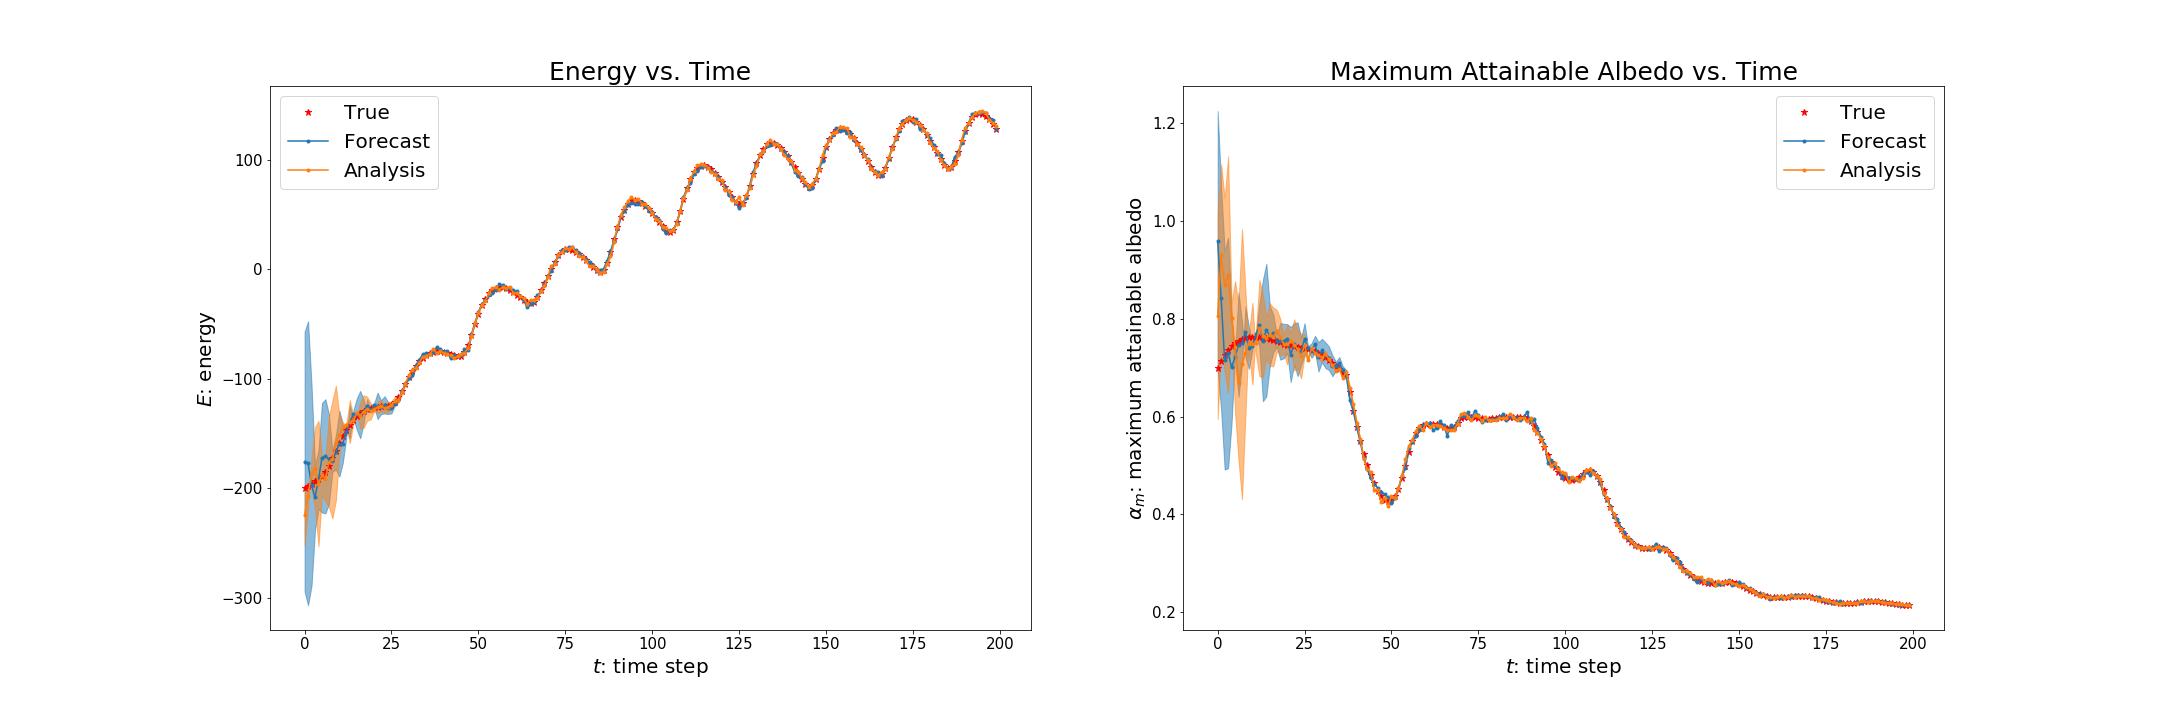
\includegraphics[width=\linewidth]{Figures/H_true_new.png} 
\end{center}
\caption{DA experiment with $\cH$, the true observation operator.}
\end{figure}


\par \figref{hmlhatDA} plots the performance of data assimilation with $\hmlhat$, the machine learning observation operator trained with an unrealistically large amount of data. We can barely tell the difference between $\hmlhat$ and the true observation operator $\cH$, except for the different shapes of shade at the first few steps caused by randomly initializing the ensembles. Again, the forecast and analysis estimates converge to the truth after $20-30$ time steps and follow along the true trajectory thereafter. Such results demonstrate that the machine learning observation operator can achieve the same performance as the true observation operator, as long as it is provided with sufficient data.

\begin{figure}\label{fig:hmlhatDA}
\begin{center}
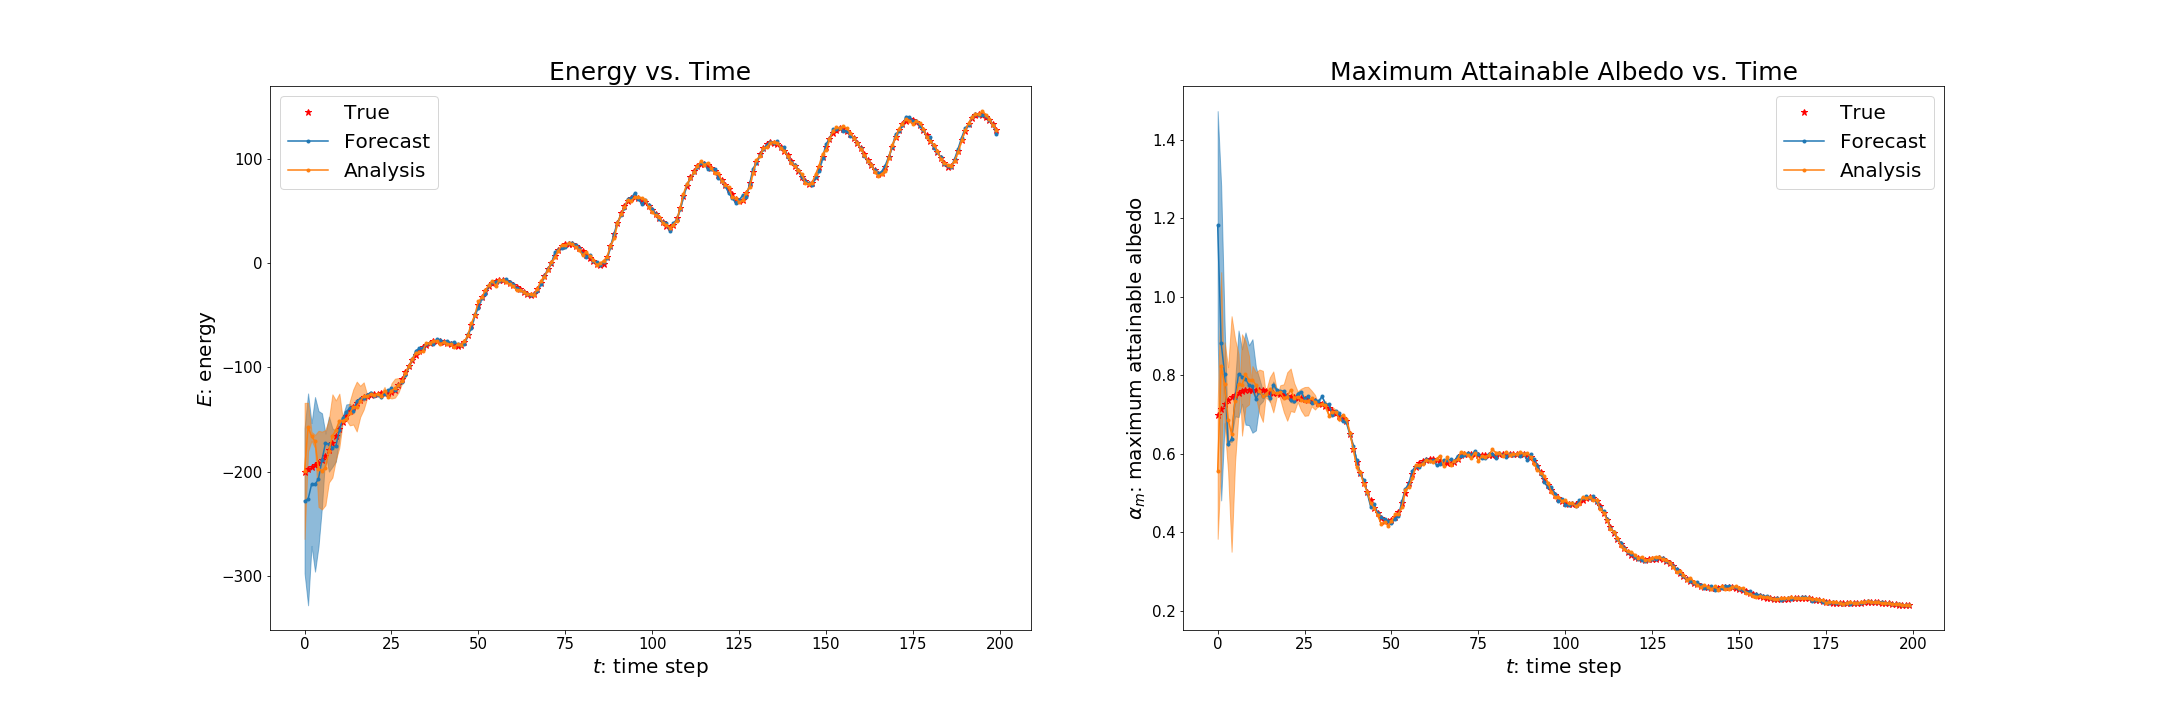
\includegraphics[width=\linewidth]{Figures/H_ml_hat_grid_new.png} 
\end{center}
\caption{DA experiment with $\hmlhat$, i.e. ML OP with grid training data.}
\end{figure}

\par \figref{hmlDA} plots the performance of data assimilation with $\hml$, the machine learning observation operator trained with data from trajectories. Comparing \figref{hmlDA} with \figref{hmlhatDA}, we can see that there is a noticeable difference at the first time steps. This is due to the lack of training data at transient states at the first time steps for $\hml$. However, we notice that after around $50$ time steps, the forecast and analysis estimates converge to the truth. On the one hand, ensemble Kalman filter generally takes time to converge. On the other hand, once the trajectories enter the area where limit cycles reside and data becomes sufficiently dense, the accuracy of the machine learning observation operator increases, leading to a corresponding improvement of performance in data assimilation. Eventually, like the experiments with $\cH$ and $\hmlhat$, the forecast and analysis values overlap with the truth and the variance becomes visibly smaller. The real world implication would be that even if we do not have enough training representing every possible physical situation or every possible configuration of the sea ice and melt ponds, we can still apply the machine learning observation operator in data assimilation.

\begin{figure}\label{fig:hmlDA}
\begin{center}
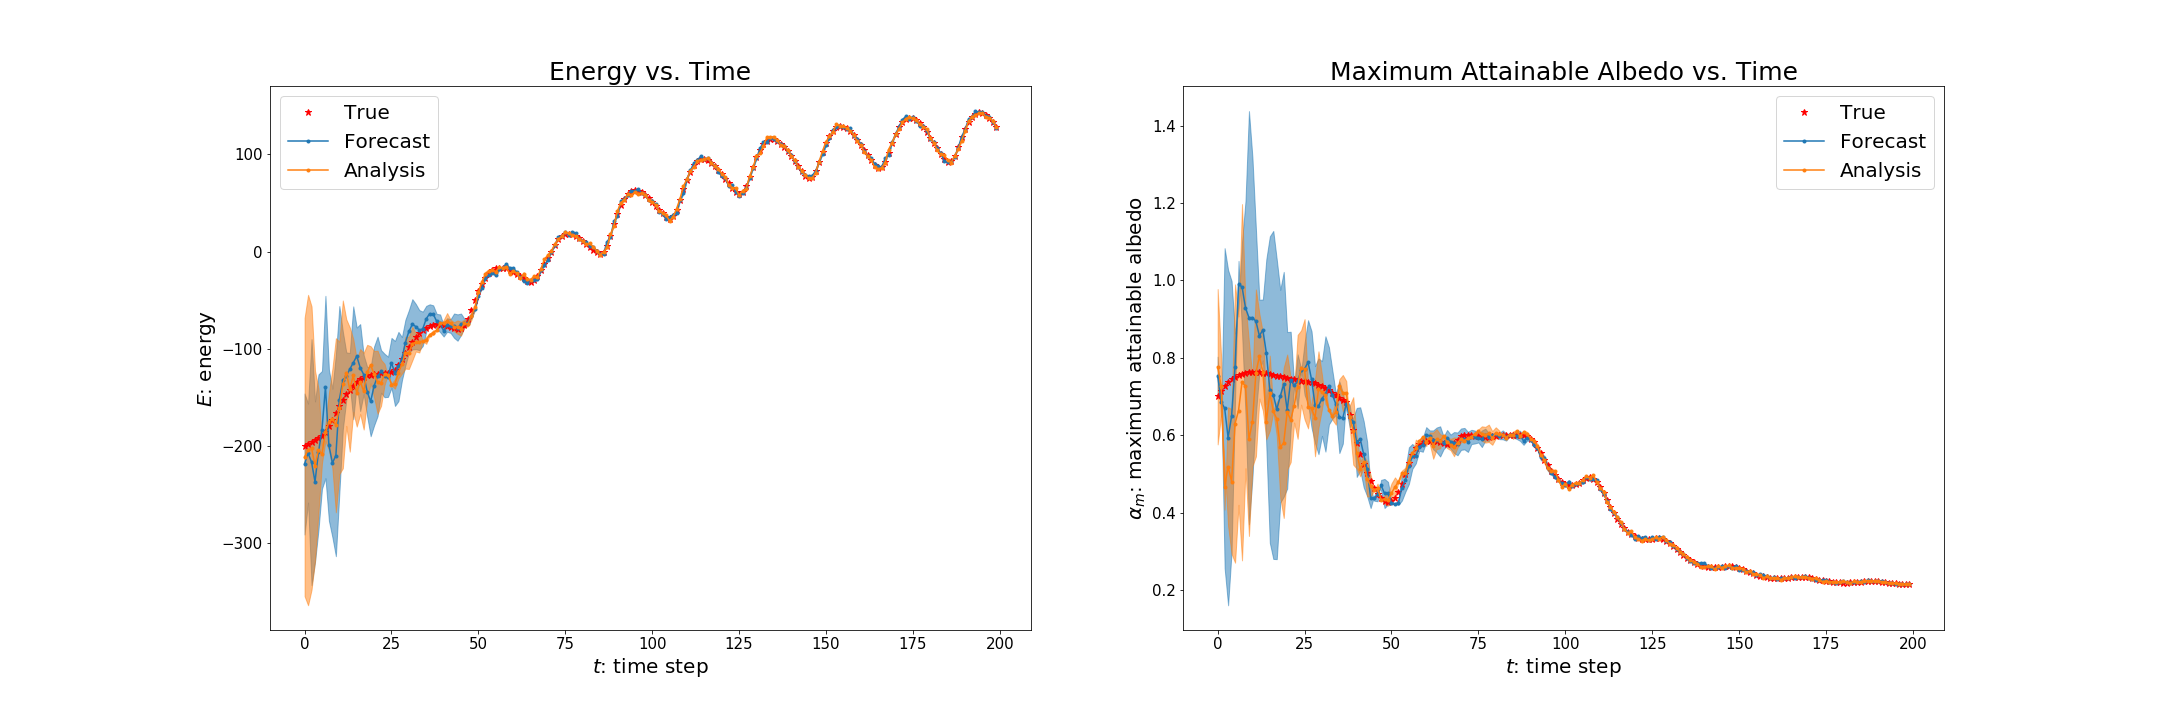
\includegraphics[width=\linewidth]{Figures/H_ml_hat_new.png} 
\end{center}
\caption{DA experiment with $\hml$, i.e. ML OP with training data from trajectories.}
\end{figure}

\par \figref{hretrievalDA} plots the performance of data assimilation with $\hretrieval$, the proxy for satellite retrieved ice concentration. Unlike the experiments with $\cH$, $\hml$, and $\hmlhat$, the forecast and analysis estimates with $\hretrieval$ never converge to the truth. Although the curves seem to follow the true dynamics, they are constantly oscillating around the true values and rarely give reasonably accurate predictions. This closely resembles the real world situation, where in the summertime, as the melt ponds start to form, the sea ice models assimilating the inaccurate sea ice concentration retrieved from satellite radiances begin to fail.

\begin{figure}\label{fig:hretrievalDA}
\begin{center}
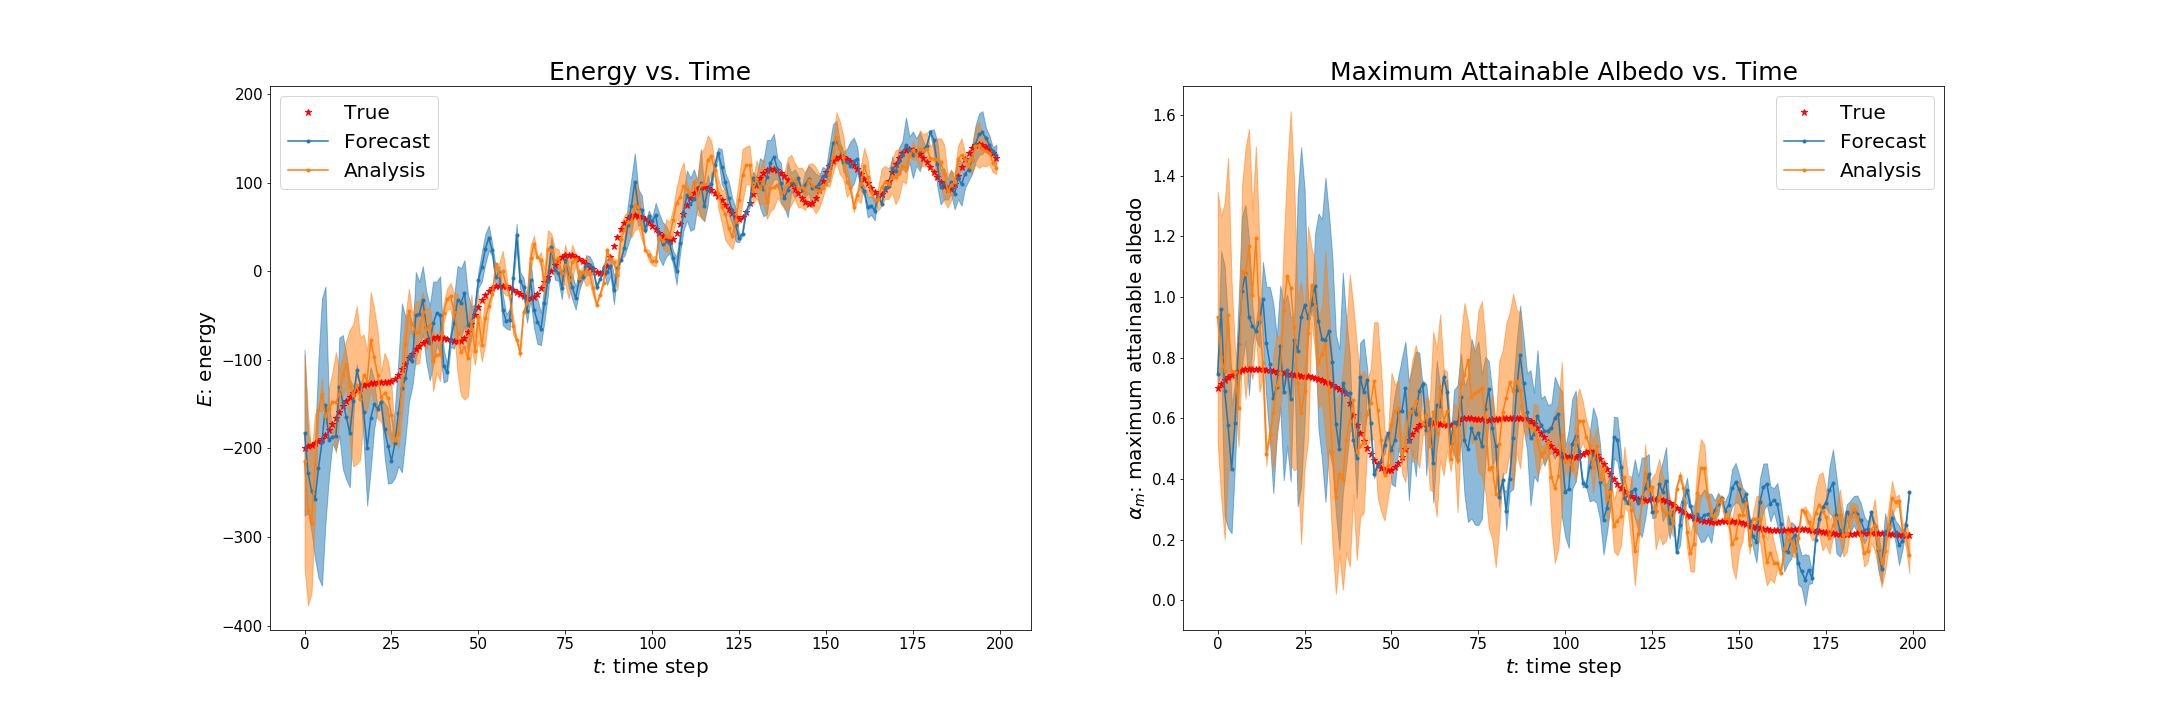
\includegraphics[width=\linewidth]{Figures/H_retrieval_new.png} 
\end{center}
\caption{DA experiment with $\hretrieval$, the observation operator representing the proxy for satellite retrieval algorithm.}
\end{figure}

\subsection{Results with Sparse Data}

\par \figref{h5pDA} and \figref{h30pDA} show the performance of data assimilation with $\hsparser$ and $\hsparse$, the machine learning observation operator trained with only $5\%$ or $30\%$ data in the region of interest. Comparing \figref{h5pDA} and \figref{h30pDA} with \figref{hmlDA} and \figref{hmlhatDA}, we can see that the performance is obviously worse in general. In particular, the estimates with $\hsparser$ does not converge to the truth after 200 steps. This shows that the severe lack of training data can cause the failure of data assimilation, especially in the regions of interest where the most important dynamics take place. However, we notice that for $\hsparse$ after around $150$ time steps, when the trajectory begins to deviate from the region of insufficient data, i.e. when $E>50$, the forecast and analysis estimates still converge to the truth. Most importantly, $\hsparse$ clearly outperforms $\hretrieval$, suggesting that machine learning is still a desirable option even in situations where the data set is incomplete.

\begin{figure}\label{fig:h30pDA}
\begin{center}
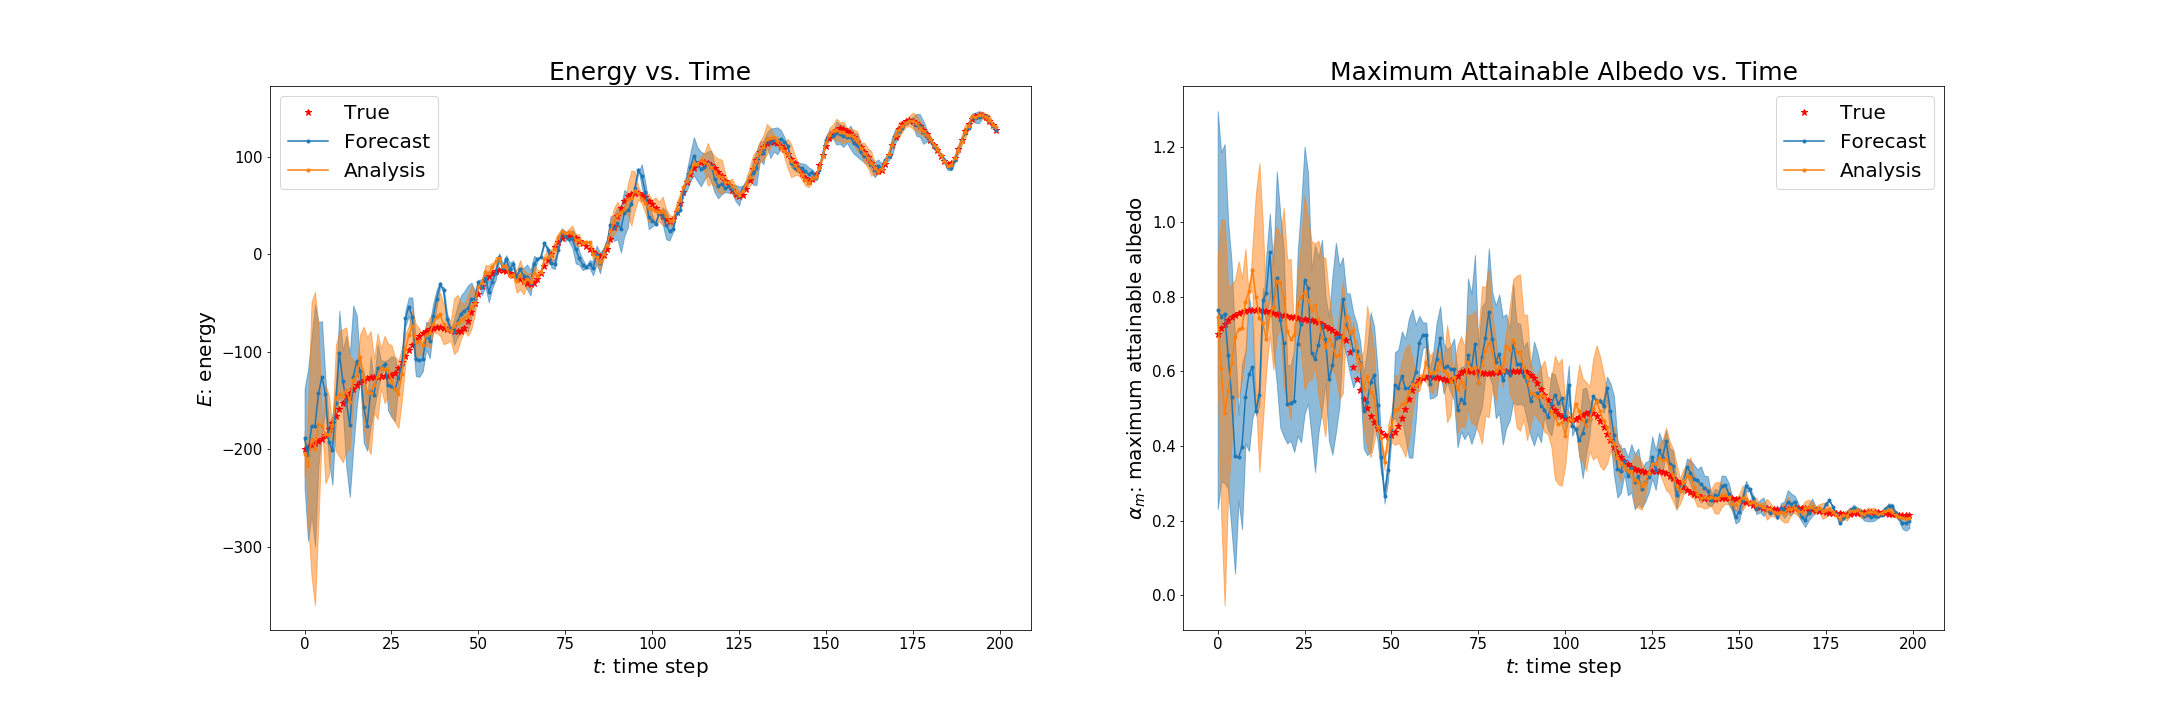
\includegraphics[width=\linewidth]{Figures/H_sparse_05_new.png} 
\end{center}
\caption{DA experiment with $\hsparse$, i.e. ML OP trained with $30\%$ data in $E\in[-50,50]$.}
\end{figure}

\begin{figure}\label{fig:h5pDA}
\begin{center}
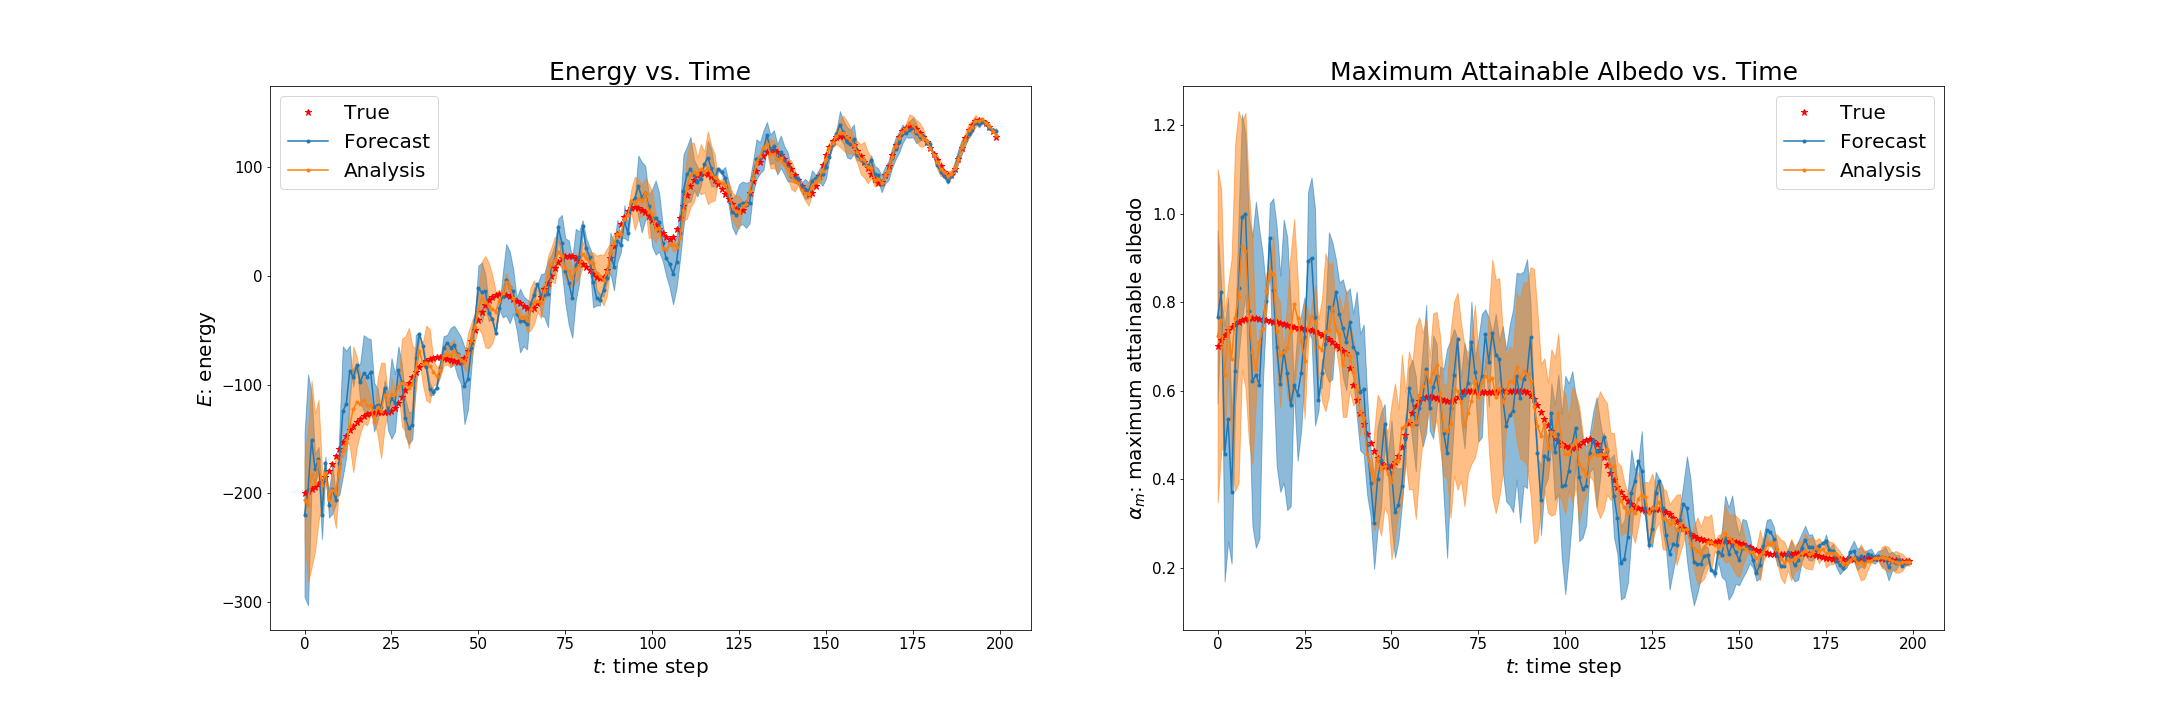
\includegraphics[width=\linewidth]{Figures/H_sparse_new.png} 
\end{center}
\caption{DA experiment with $\hsparser$, i.e. ML OP trained with $5\%$ data in $E\in[-50,50]$.}
\end{figure}

\subsection{Review and Comparison}
\par \figref{error_am_1} and \figref{error_E_1} compare the performance of different observation operators in terms of forecast and analysis absolute error in $E$ and $\am$ at each time step. Obviously, data assimilation with the retrieved concentration performs far worse than the others. 

\begin{figure}\label{fig:error_am_1}
\centering
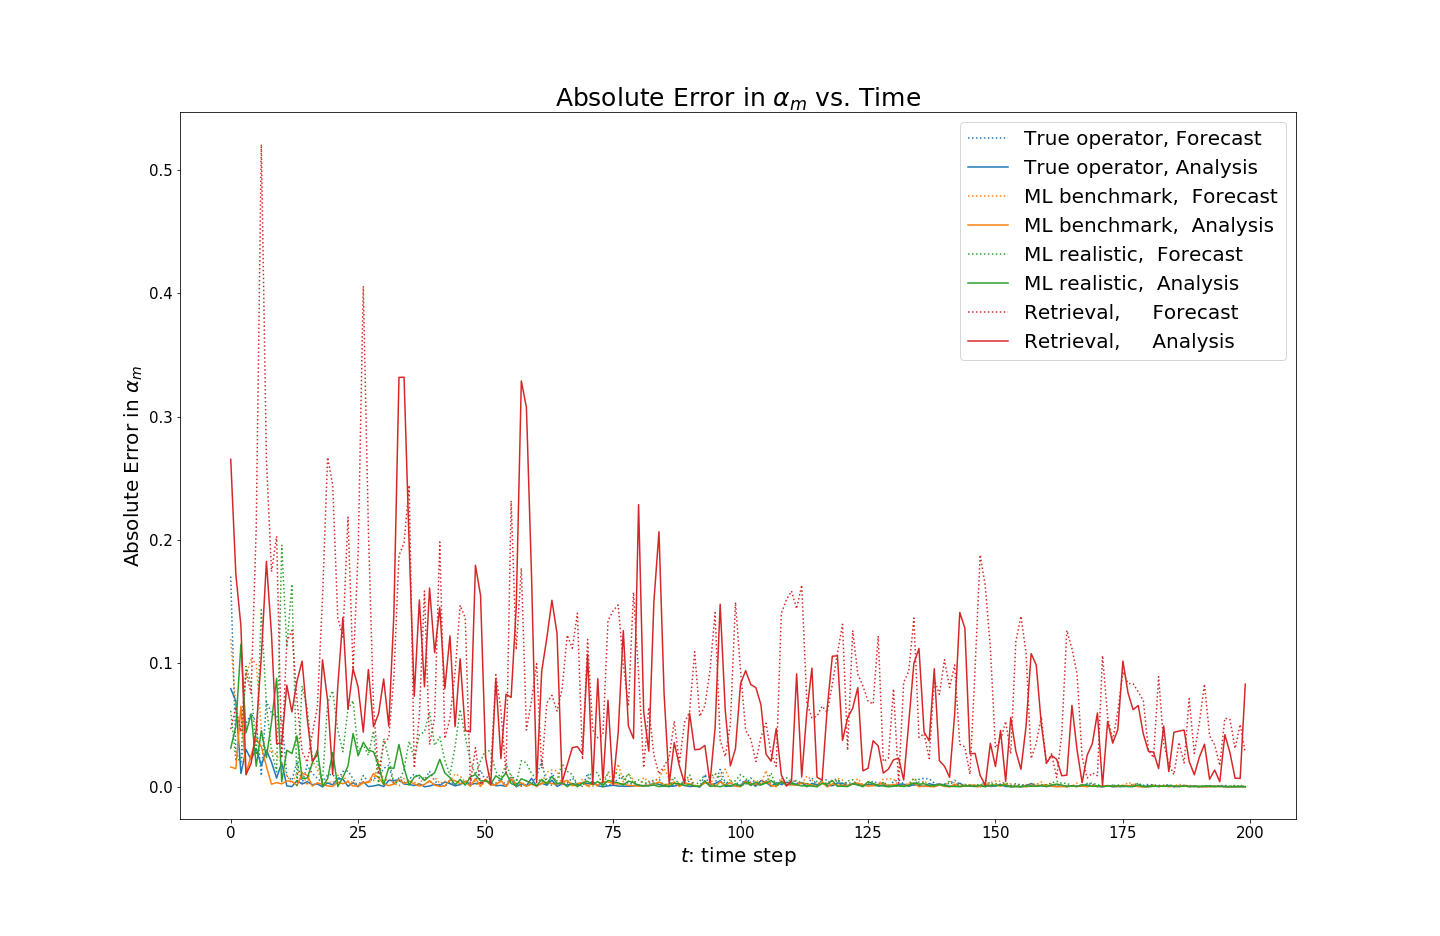
\includegraphics[width=\linewidth]{Figures/AbsoluteError_am.png}
\caption{Time evolution of absolute error of $\alpha_m$ with $\cH$, $\hmlhat$, $\hml$, and $\hretrieval$, respectively}
\end{figure}

\begin{figure}\label{fig:error_E_1}
\centering
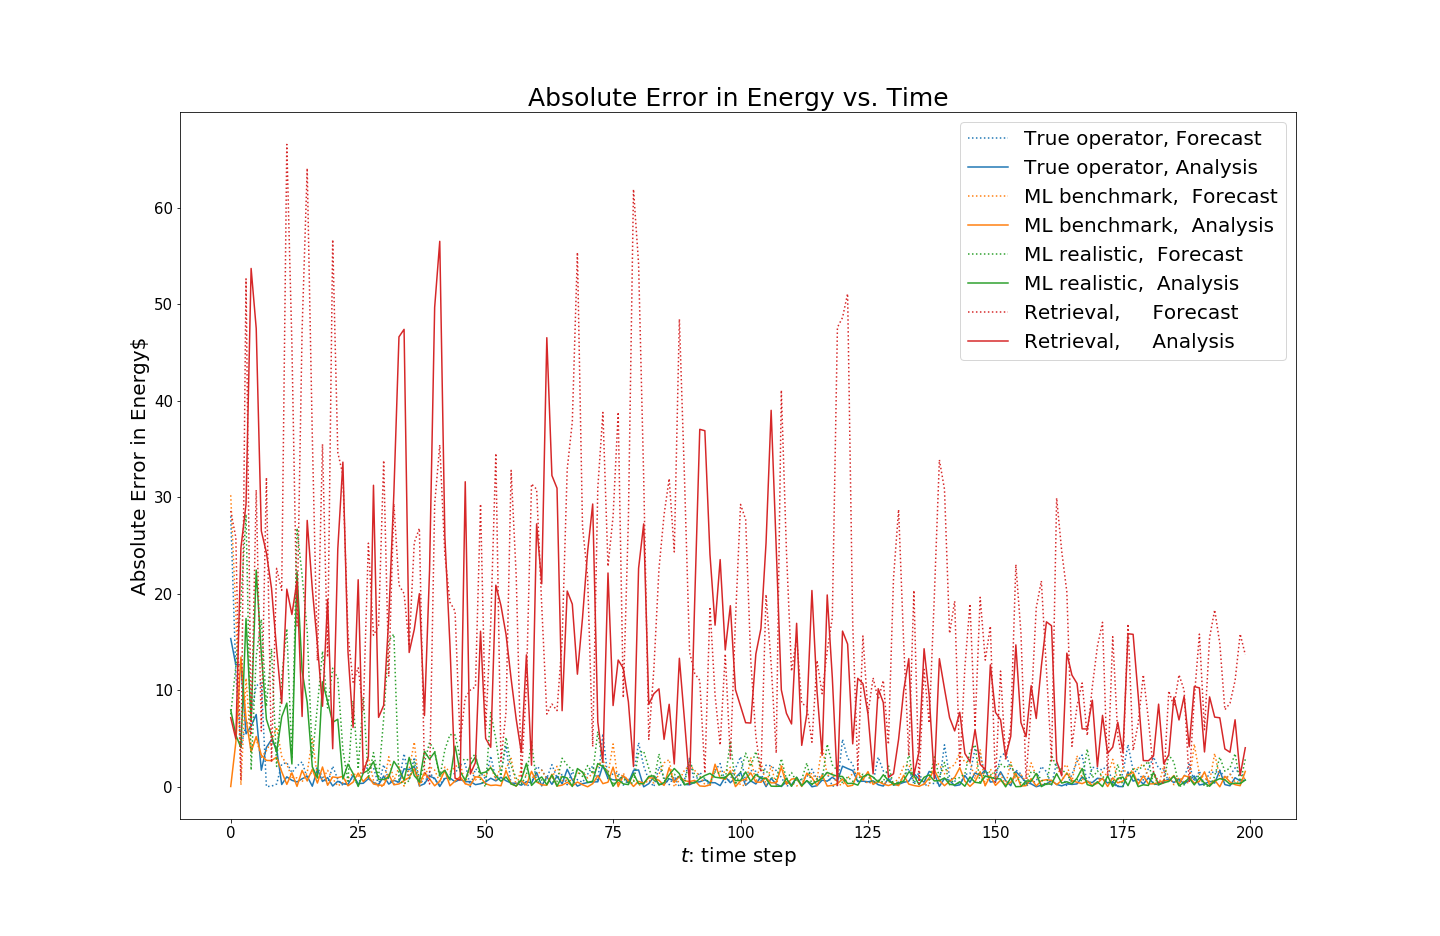
\includegraphics[width=\linewidth]{Figures/AbsoluteError_E.png}
\caption{Time evolution of absolute error of $E$ with $\cH$, $\hmlhat$, $\hml$, and $\hretrieval$, respectively}
\end{figure}

\par \figref{error_am_2} and \figref{error_E_2}, after removing $\hretrieval$, provide a clearer illustration of how assimilating using the machine learning observation operator performs. We can see that the behavior in $E$ and $\alpha_m$ are consistent. Around the first 30 time steps, $\hml$ does not perform very well. This is expected since, initially, the system is in transient states where the machine learning algorithm does not have sufficient data to learn the true observation operator. After a while, the error of $\hml$ decreases to roughly the same as $\cH$ and $\hmlhat$.

\begin{figure}\label{fig:error_am_2}
\centering
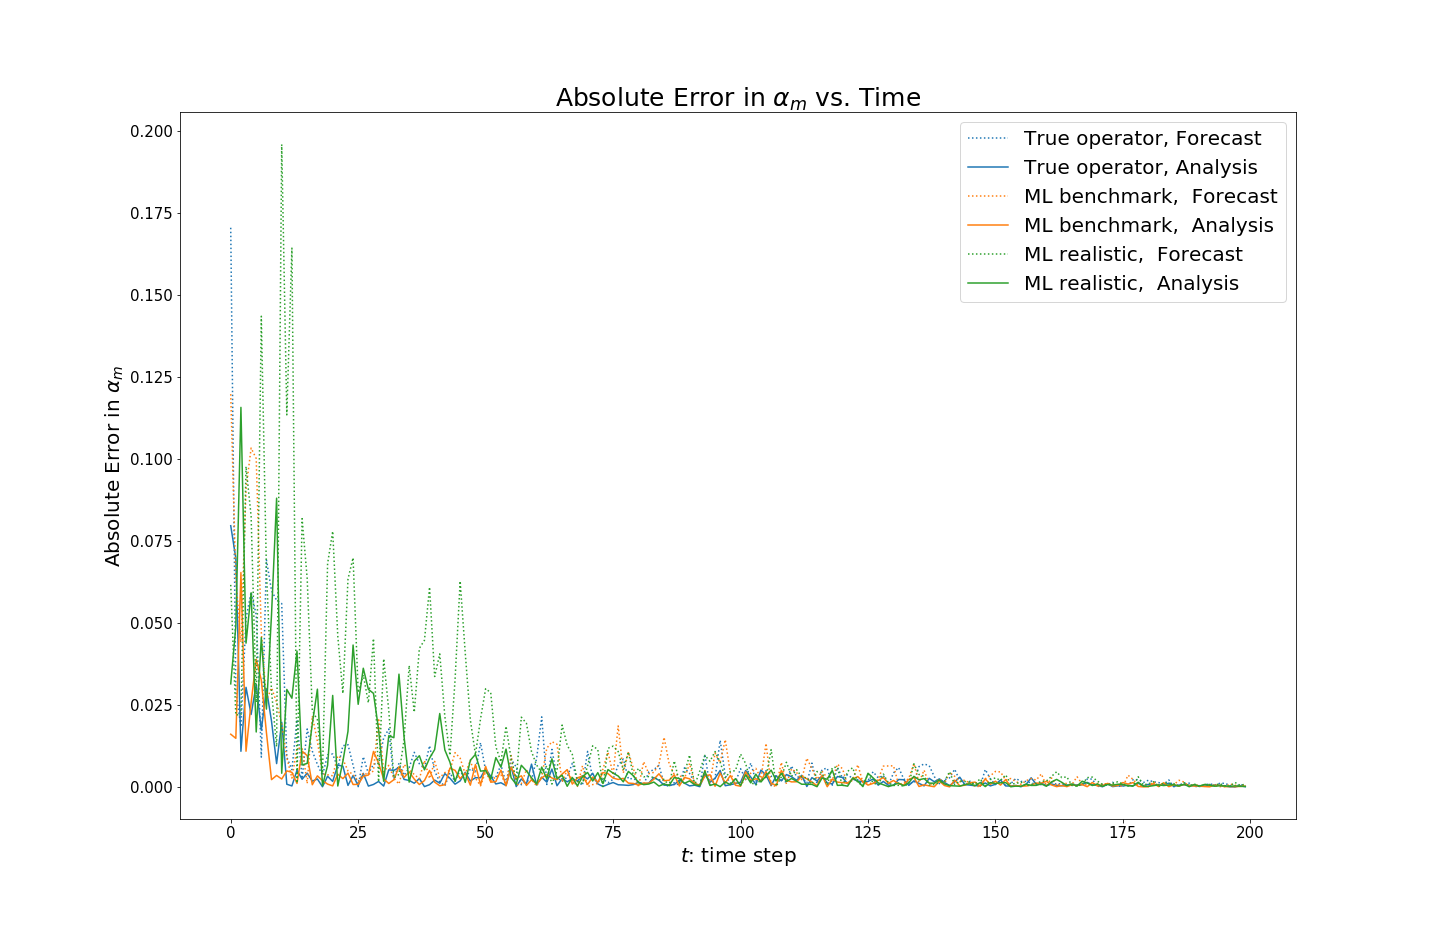
\includegraphics[width=\linewidth]{Figures/AbsoluteError_am_2.png}
\caption{Time evolution of absolute error of $\alpha_m$ with $\cH$, $\hmlhat$, and $\hml$, respectively}
\end{figure}

\begin{figure}\label{fig:error_E_2}
\centering
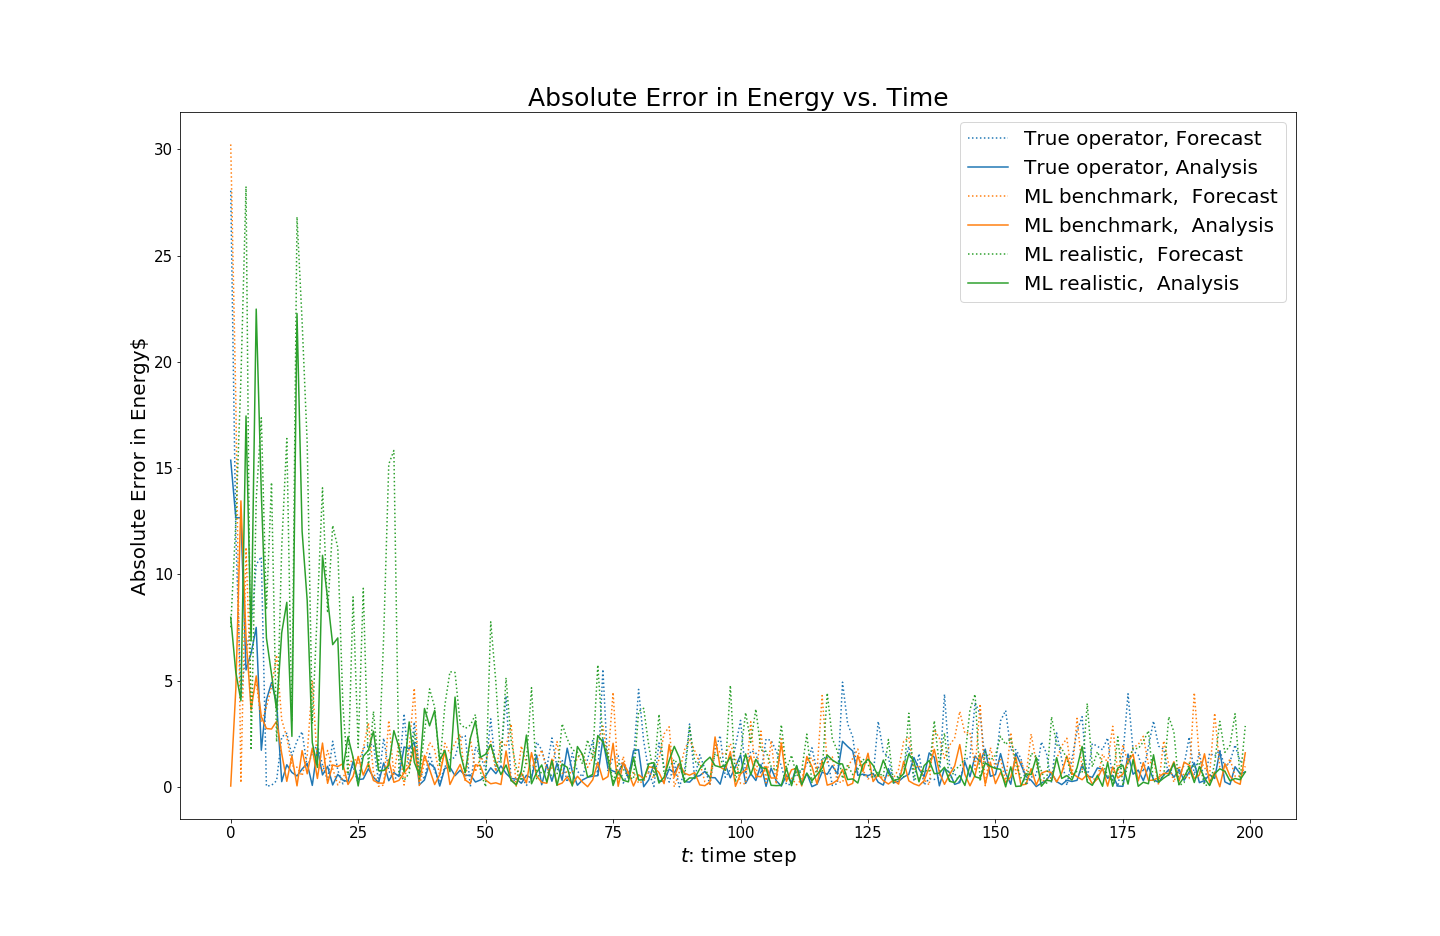
\includegraphics[width=\linewidth]{Figures/AbsoluteError_E_2.png}
\caption{Time evolution of absolute error of $E$ with $\cH$, $\hmlhat$, and $\hml$, respectively}
\end{figure}

\chapter{Discussion}
\section{Conclusions}
\par In this study, we built a test bed model proxy in \chref{formulation} for the melt pond problem in sea ice concentration retrieval, along with proxies for ice and pond concentration and satellite radiances. Our model roughly mimics the actual physical processes and give us interesting behaviors to investigate.

\par We generated several data sets to train machine learning observation operators for different purposes in \secref{datageneration}. The machine learning algorithm approximates the true observation operator reasonably well. With a sufficient amount of data, it is able to achieve roughly the same performance as the true observation operator. While its performance severely affected by the amount of data available, where in transient states, without sufficient data, the machine learning observation operator could make large errors, we were able to find a way of quantifying the accuracy with data density and averaged test error in the grided state space \secref{DataDensity}.

\par The DA experiments in \chref{experiments} demonstrate that in our testbed model, assimilating directly on the proxy for satellite radiances with machine learning observation operator works well and far outperforms assimilating on the proxy for inaccurately retrieved sea ice concentration. Even for models trained with sparse data, the performance is still better than assimilating with wrong concentration. We can use the performance on the test set and data density to estimate the error covariance matrix of machine learning observation operator and apply covariance inflation accordingly at corresponding locations in the phase space. 

\par In conclusion, for data assimilation in sea ice concentration with melt ponds, it is a desirable option to use historic data to construct a machine learning observation operator taking the state variables directly to the satellite radiances. Even if only a small amount of historic data is available for training or the data is highly noisy, machine learning is still likely to offer a better solution than satellite retrieval algorithm.

\section{Future Direction}
\par The scope of the study is limited by the time we have, so we only tested with one machine learning algorithm, that is the neural network, and one data assimilation scheme, the ensemble Kalman filter. To fully explore the potential advantages and challenges in our idea, we will try using other machine learning algorithms like XGBoost and Random Forest. Furthermore, since our system is low dimensional and highly non-linear, the particle filter is a reasonable choice to do data assimilation with.
\par In this study, we demonstrated our idea on a simple testbed model. The first step is successful, and starting from here, we will test our idea on larger scale models that are actually used in the reality, e.g. The Community Sea Ice Model (CSIM) \cite{CICE} along with an atmospheric radiative transfer model that computes the actual satellite radiances from state variables.  The major challenges would be first, the dimension of the real systems is significantly larger, second the computational cost would be much higher, and third, it is in question whether machine learning would still be able to approximate the complicated atmospheric model.
\par The eventual goal of our study is to build a machine learning model that takes sea ice states to the satellite radiances. The first step is to gather data of matching instances where we know pond and open water fraction with passive microwave measurements we could generate a training set. MOSAiC - The Multidisciplinary Drifting Observatory for the Study of Arctic Climate is a mission which may provide some data like this.
\clearpage
\phantomsection

{\def\chapter*#1{} % suppress bibliograph header.
\begin{singlespace}
\addcontentsline{toc}{chapter}{BIBLIOGRAPHY}
\begin{center}
\Large \textbf{BIBLIOGRAPHY}
\vspace{17pt}
\end{center}

\bibliographystyle{apalike}
\bibliography{common/reference.bib}
\end{singlespace}
}





\end{document}
